%
% Template Laporan Skripsi/Thesis
%
% @author  Andreas Febrian, Lia Sadita
% @version 1.03
%
% Dokumen ini dibuat berdasarkan standar IEEE dalam membuat class untuk
% LaTeX dan konfigurasi LaTeX yang digunakan Fahrurrozi Rahman ketika
% membuat laporan skripsi. Konfigurasi yang lama telah disesuaikan dengan
% aturan penulisan thesis yang dikeluarkan UI pada tahun 2008.
%

%
% Tipe dokumen adalah report dengan satu kolom.
%
% \documentclass[12pt, a4paper, onecolumn, oneside, final]{report}
\documentclass[12pt, a4paper, onecolumn, oneside, draft]{report}

% Load konfigurasi LaTeX untuk tipe laporan thesis
\usepackage{_internals/uithesis}
\usepackage{enumitem}
\usepackage{bm}
\usepackage{multirow}
\usepackage{longtable}
\usepackage{booktabs,array,dcolumn}
\usepackage{threeparttablex}
\usepackage[natbibapa]{apacite}
\usepackage{doi}

\newcolumntype{d}{D{.}{.}{2.3}}
\newcolumntype{C}{>{\centering}p}

\newcommand{\footlabel}[2]{%
    \addtocounter{footnote}{1}%
    \footnotetext[\thefootnote]{%
        \addtocounter{footnote}{-1}%
        \refstepcounter{footnote}\label{#1}%
        #2%
    }%
    $^{\ref{#1}}$%
}

\newcommand{\footref}[1]{%
    $^{\ref{#1}}$%
}


% Load konfigurasi khusus untuk laporan yang sedang dibuat
%-----------------------------------------------------------------------------%
% Informasi Mengenai Dokumen
%-----------------------------------------------------------------------------%
%
% Judul laporan.
\var{\judul}{A Benchmarking Tool for Computational Reproducibility}
%
% Tulis kembali judul laporan, kali ini akan diubah menjadi huruf kapital
\Var{\Judul}{A Benchmarking Tool for Computational Reproducibility}
%
% Tulis kembali judul laporan namun dengan bahasa Ingris
\var{\judulInggris}{A Benchmarking Tool for Computational Reproducibility}

%
% Tipe laporan, dapat berisi Skripsi, Tugas Akhir, Thesis, atau Disertasi
\var{\type}{Thesis}
%
% Tulis kembali tipe laporan, kali ini akan diubah menjadi huruf kapital
\Var{\Type}{Thesis}

\var{\fullType}{Bachelor Thesis}
\Var{\FullType}{Bachelor Thesis}
%
% Tulis nama penulis
\var{\penulis}{Rakha Kanz Kautsar}
%
% Tulis kembali nama penulis, kali ini akan diubah menjadi huruf kapital
\Var{\Penulis}{Rakha Kanz Kautsar}
%
% Tulis NPM penulis
\var{\npm}{1506688784}
%
% Tuliskan Fakultas dimana penulis berada
\Var{\Fakultas}{Computer Science}
\var{\fakultas}{Computer Science}
%
% Tuliskan Program Studi yang diambil penulis
\Var{\Program}{Computer Science}
\var{\program}{Computer Science}
%
% Tuliskan tahun publikasi laporan
\Var{\bulan}{Juli}
\Var{\tahun}{2019}
%
% Tuliskan gelar yang akan diperoleh dengan menyerahkan laporan ini
\var{\gelar}{Bachelor of Computer Science}
%
% Tuliskan tanggal pengesahan laporan, waktu dimana laporan diserahkan ke
% penguji/sekretariat
\var{\tanggalPengesahan}{XX Juli 2019}
%
% Tuliskan tanggal keputusan sidang dikeluarkan dan penulis dinyatakan
% lulus/tidak lulus
\var{\tanggalLulus}{XX Juli 2019}
%
% Tuliskan pembimbing
\var{\pembimbing}{Drs. Lim Yohanes Stefanus, M.Math., Ph.D}
\var{\pembimbingDua}{Dr. Johannes K. Fichte}
%
% Alias untuk memudahkan alur penulisan paa saat menulis laporan
\var{\saya}{Penulis}
\var{\First}{We}
\var{\first}{we}
\var{\firstposs}{our}
\var{\Firstposs}{Our}

%-----------------------------------------------------------------------------%
% Judul Setiap Bab
%-----------------------------------------------------------------------------%
%
% Berikut ada judul-judul setiap bab.
% Silahkan diubah sesuai dengan kebutuhan.
%
\Var{\kataPengantar}{Preface}
\Var{\chIntroduction}{Introduction}
\Var{\chExperimentation}{Experimentation \& Benchmarking}
\Var{\chResource}{Measuring \& Limiting Resource}
\Var{\chExisting}{Existing Benchmarking Tools}
\Var{\chImplementation}{Implementation}
\Var{\chEvaluation}{Evaluation}
\Var{\chConclusion}{Conclusion \& Future Works}


\usetikzlibrary{shapes,arrows,positioning,fit,backgrounds}

% Daftar istilah yang mungkin perlu ditandai
%
% @author  Andreas Febrian
% @version 1.00
% 
% Mendaftar seluruh istilah yang mungkin akan perlu dijadikan 
% italic atau bold pada setiap kemunculannya dalam dokumen. 
% 

\var{\license}{\f{Creative Common License 1.0 Generic}}
\var{\bslash}{$\setminus$}

% Awal bagian penulisan laporan
\begin{document}
%
% Sampul Laporan
%
% Sampul Laporan

%
% @author  unknown
% @version 1.01
% @edit by Andreas Febrian
%

\begin{titlepage}
    \begin{center}    
        \begin{figure}
            \begin{center}
                
\includegraphics[width=2.5cm]{_internals/makara.eps}
            \end{center}
        \end{figure}    
        \vspace*{0cm}
        \bo{
        	UNIVERSITAS INDONESIA\\
        }
        
        \vspace*{1.0cm}
        % judul thesis harus dalam 14pt Times New Roman
        \bo{\Judul} \\[1.0cm]

        \vspace*{2.5 cm}    
        % harus dalam 14pt Times New Roman
        \bo{\Type}

        \vspace*{3 cm}       
        % penulis dan npm
        \bo{\Penulis} \\
        \bo{\npm} \\

        \vspace*{5.0cm}

        % informasi mengenai fakultas dan program studi
        \bo{
        	FAKULTAS \Fakultas\\
        	PROGRAM STUDI \Program \\
        	DEPOK \\
        	\tahun
        }
    \end{center}
\end{titlepage}


%
% Gunakan penomeran romawi
\pagenumbering{roman}

%
% load halaman judul dalam
\addChapter{TITLE PAGE}
%
% Halaman Judul Laporan 
%
% @author  unknown
% @version 1.01
% @edit by Andreas Febrian
%

\begin{titlepage}
    \begin{center}\begin{figure}
            \begin{center}
                
\includegraphics[width=2.5cm]{_internals/makara.eps}
            \end{center}
        \end{figure}    
        \vspace*{0cm}
        \bo{
        	UNIVERSITAS INDONESIA\\
        }
        
        \vspace*{1.0cm}
        % judul thesis harus dalam 14pt Times New Roman
        \bo{\Judul} \\[1.0cm]

        \vspace*{2.5 cm}    
        % harus dalam 14pt Times New Roman
        \bo{\FullType} \\
        % keterangan prasyarat
        \bo{A thesis submitted in partial fulfillment of the requirements for the degree of \\
        \gelar}\\

        \vspace*{3 cm}       
        % penulis dan npm
        \bo{\Penulis} \\
        \bo{\npm} \\

        \vspace*{5.0cm}

        % informasi mengenai fakultas dan program studi
        \bo{
        	FACULTY OF \Fakultas\\
        	STUDY PROGRAM OF \Program \\
        	DEPOK \\
        	\bulan\ \tahun
        }
    \end{center}
\end{titlepage}

%
% setelah bagian ini, halaman dihitung sebagai halaman ke 2
\setcounter{page}{2}

%
% load halaman pengesahan
\addChapter{APPROVAL PAGE}
%
% Halaman Pengesahan
%
% @author  Andreas Febrian
% @version 1.01
%

\chapter*{Approval Page}

\vspace*{0.2cm}
\noindent 

\noindent
\begin{tabular}{l l p{11cm}}
	\bo{Title}&: & \judul \\ 
	\bo{Name}&: & \penulis \\
	\bo{NPM}&: & \npm \\
\end{tabular} \\

\vspace*{1.2cm}

\noindent This thesis has been examined and approved.\\[0.3cm]
\begin{center}
\tanggalPengesahan \\[2cm]


\underline{\pembimbing}\\[0.1cm]
Pembimbing \type
\end{center}

\newpage
%
% load halaman orisinalitas
\addChapter{STATEMENT OF ORIGINALITY}
%
% Halaman Orisinalitas
%
% @author  Andreas Febrian
% @version 1.01
%

\chapter*{Halaman Pernyataan Orisinalitas}
\vspace*{2cm}

\begin{center}
	\bo{\type~ini adalah hasil karya saya sendiri, \\ 
	dan semua sumber baik yang dikutip maupun dirujuk \\
	telah saya nyatakan dengan benar.} \\
	\vspace*{2.6cm}
	
	\begin{tabular}{l c l}
	\bo{Nama} & : & \bo{\penulis} \\
	\bo{NPM} & : & \bo{\npm} \\ 
	\bo{Tanda Tangan} & : & \\
	& & \\
	& & \\
	\bo{Tanggal} & : & \bo{\tanggalPengesahan} \\	
	\end{tabular}
\end{center}

\newpage
%
%
\addChapter{CERTIFICATION OF APPROVAL}
%
% Halaman Pengesahan Sidang
%
% @author  Andreas Febrian, Andre Tampubolon 
% @version 1.02
%

\chapter*{Certification of Approval}

\vspace*{0.4cm}
\noindent 

\noindent
\begin{tabular}{ll p{9cm}}
	This thesis, submitted by&: & \\
	Name&: & \penulis \\
	NPM&: & \npm \\
	Study Program&: & \program \\
	\type~Title&: & \judul \\
\end{tabular} \\

\vspace*{1.0cm}

\noindent \bo{Has successfully been defended in the presence of Board of
Examiners and accepted in partial fulfillment of the requirements for
the degree of \gelar~ at the Study Program of \program, Faculty of \fakultas,
Universitas Indonesia}\\[0.2cm]

\begin{center}
	\bo{Board of Examiners}
\end{center}

\vspace*{0.3cm}

\begin{tabular}{l l l l }
	& & & \\
	Supervisor&: & \pembimbing & (\hspace*{3.0cm}) \\
	& & & \\
	Co-supervisor&: & \pembimbingDua & (\hspace*{3.0cm}) \\
	& & & \\
	Examiner&: & & (\hspace*{3.0cm}) \\
	& & & \\
	Examiner&: & & (\hspace*{3.0cm}) \\
\end{tabular}\\

\vspace*{2.0cm}

\begin{tabular}{ll l}
	Signed at&: & Depok\\
	Date&: & \tanggalLulus \\
\end{tabular}


\newpage
%
%
\addChapter{PREFACE}
%-----------------------------------------------------------------------------%
\chapter*{Preface}
%-----------------------------------------------------------------------------%

\todo{preface}

First and foremost, we would like to thank 

\vspace*{0.1cm}
\begin{flushright}
Dresden, 14 June 2019\\[0.1cm]
\vspace*{1cm}
\penulis

\end{flushright}
%
%
\clearpage
\addChapter{STATEMENT OF CONSENT OF ACADEMIC PUBLICATION}
% 
% @author  Andre Tampubolon, Andreas Febrian
% @version 1.01
% 

\chapter*{Statement of Consent of Thesis Publication for Academic Interests}

\vspace*{0.2cm}
\noindent 
As a member of academic community of Universitas Indonesia,
I the undersigned below:
\vspace*{0.4cm}


\begin{tabular}{p{4.2cm} l p{6cm}}
	\bo{Name} & : & \penulis \\ 	
	\bo{NPM} & : & \npm \\
	\bo{Study Program} & : & \program\\	
	\bo{Faculty} & : & \fakultas\\
	\bo{Academic Work} & : & \type~(S1) \\
\end{tabular}

\vspace*{0.6cm}
\noindent in the scientific development interests, hereby consent to grant
Universitas Indonesia a \bo{\textit{Non‐exclusive Royalty‐Free Right}}
my scientific work entitled:

\begin{center}
	\judul
\end{center}

\noindent~along with its existing sets of supplementary materials (if required).
With Non‐exclusive Royalty‐Free Right, Universitas Indonesia has rights
to save, media‐transfer/format, manage in a database, maintain, and
publish my final project provided my name is retained as the author/creator
and the owner of Copyright. \\

\noindent I certify that the statement is true to the best of my knowledge

\begin{center}
	\vspace*{0.8cm}
	\begin{tabular}{rl}
		Signed at : & Depok \\
		Date : & \tanggalPengesahan \\
	\end{tabular}\\

	\vspace*{0.2cm}
	Signed \\
	\vspace*{1.1cm}
	(\penulis)
\end{center}

\newpage


%
%
\addChapter{ABSTRACT}
%
% Halaman Abstract
%
% @author  Andreas Febrian
% @version 1.00
%

\chapter*{Abstract}

\vspace*{0.2cm}
{
	\setlength{\parindent}{0pt}

	\begin{tabular}{@{}l l p{10cm}}
		Name&: & \penulis \\
		Study Program&: & \program \\
		Title&: & \judulInggris \\
		Supervisors&: & \pembimbing \\
				   &  & \pembimbingDua \\
	\end{tabular}

	\bigskip
	\bigskip

	The focus of this study is the freshman student of Faculty of Psychology at University of
	Indonesia experience of acquiring, evaluating and using information, when they enroll in
	“Program Dasar Pendidikan Tinggi (PDPT)”. The purpose of this study is to understand
	how freshman students acquire, evaluate and use information. Knowing this will allow
	library to identify changes should be made to improve user education program at
	University of Indonesia. This research is qualitative descriptive interpretive. The data
	were collected by means of deep interview. The researcher suggests that library should
	improve the user education program and provide facilities which can help students to be
	information literate.

	\bigskip

	Key words:\\
	Information literacy, information skills, information
}

\newpage
%
%
%
% Halaman Abstrak
%
% @author  Andreas Febrian
% @version 1.00
%

\chapter*{Abstrak}

\vspace*{0.2cm}
{
	\setlength{\parindent}{0pt}
	
	\begin{tabular}{@{}l l p{10cm}}
		Nama&: & \penulis \\
		Program Studi&: & \program \\
		Judul&: & \judul \\
		Pembimbing&: & \pembimbing \\
				  &  & \pembimbingDua \\
	\end{tabular}

	\bigskip
	\bigskip

	Tesis ini membahas kemampuan mahasiswa Fakultas Psikologi UI dalam mencari dan
	menggunakan informasi secara efektif dalam konteks \textit{active learning} dan \textit{self regulated
	learning} selama mereka mengikuti Program Pendidikan Dasar Pendidikan Tinggi.
	Penelitian ini adalah penelitian kualitatif dengan desain deskriptif. Hasil penelitian
	menyarankan bahwa perpustakaan perlu dilibatkan dalam pengembangan kurikulum;
	materi pendidikan pemakai perpustakaan harus dikembangkan sesuai dengan komponen-
	komponen yang ada dalam \textit{information literacy}; perpustakaan juga harus menyediakan
	sarana dan fasilitas yang mendukung peningkatan \textit{literacy} mahasiswa.

	\bigskip

	Kata kunci:\\
	Informasi, \textit{information literacy}, \textit{information skills}
}

\newpage

%
% Daftar isi, gambar, dan tabel
%
\phantomsection
\tableofcontents
\clearpage
\phantomsection
\listoffigures
\clearpage
\phantomsection
\listoftables
\clearpage
\phantomsection
\addcontentsline{toc}{chapter}{\uppercase{List of Listings}}
\listoflistings
\clearpage

%
% Gunakan penomeran Arab (1, 2, 3, ...) setelah bagian ini.
%
\pagenumbering{arabic}

%
%
%
\chapter{\chIntroduction}
\label{ch:introduction}


% \section{Motivation}


\citet{gowerScientificMethodHistorical2012} describe the famous thought experiment by Galileo Galilei.
The claim was as follows.
Take two objects, one lighter and the other heavier in weight.
Then tie and drop them together from the top of a tower.
If, like many have believed at that time, heavier object fall faster then the lighter one will pull the heavier one and slow down the fall.
But instead this new tied object is heavier than both and should have fallen faster.
This is a contradiction.
Thus, Galileo postulated that this phenomenon was due to air resistance and friction, independent of the object mass.
This example shows that experiment can also take place in the mind and does not have to be physical.

Experiments have also demonstrated that artificial neural network performance is better than \newstyle{what was predicted in theory} \citep{tichyShouldComputerScientists1998}.
\newcontent{Today, artificial neural networks are used in a number of surprising real-world applications.
Its applications include image recognition, speech recognition, natural language understanding, and even self-driving cars \citep{lecunDeepLearning2015}.}

\newcontent{
The Boolean Satisfiability (SAT) problem has been proven to be $\textbf{NP}$-complete by \citet{cook1971complexity} and \citet{levin1973universal} independently.
This means that SAT solving algorithms have exponential worst case running time.
\citet{nordstromPebbleGamesProof2013} remarks that most modern solvers are based on Davis-Putnam-Logemann-Loveland (DPLL) backtracking procedure from the 1960s with augmented clause learning, also known as conflict-driven clause learning (CDCL).
He further remarks that it is not yet fully understood why these solvers can be so efficient in practice \citep{elffersTradeoffsTimeMemory2016}.
This can be seen from the majority solvers submitted to the annual international SAT competition being CDCL-based, and successfully solving problems with millions of literals and clauses \citep{heule2018proceedings}.
}

And last but not least, Isaac Eddington conducted an expensive validation in 1919 to prove Einstein's theory that gravity bends light.
This important experiment involves expedition to Principe Island, West Africa and pushed the limits of photographic emulsion technology \citep{tichyShouldComputerScientists1998}.
\newstyle{Today, 100 years after the validation, this is further supported by another great advancement in astronomy.}
In April 10th 2019, the Event Horizon Telescope (EHT) presented to the public the first ever successful image of a black hole, an object predicted by Einstein's general theory of relativity \citep{akiyama2019first}.

All these examples show that experimentation has contributed to several important breakthrough in various disciplines in science.
Computational science specifically has seen a wide use of benchmarking as one way to conduct the experiment as shown in the above neural network and SAT example.
Benchmarking allow automated execution of many repeated experiments.
This automation is convenient to help tackle the recent concern of reproducibility.

\citet{gundersenStateArtReproducibility2018} and \citet{collbergRepeatabilityComputerSystems2016} both report that only a small number of researches are reproducible.
They linked this concern with the effort it takes to make a research work reproducible.
That is why we deemed it necessary to survey if the existing benchmarking tools may help with this concern.
We also tried to improve the state by contributing to the existing or even create a new benchmarking tool altogether.
This is further motivated after we see that the development of some of these benchmarking tools are often requirement-driven and thus made specific to a community need and not general need.

In this chapter, we list the research questions for this thesis in \Cref{sec:intro.questions}.
Then we give pointers on how we answer these questions in \Cref{sec:intro.method}.
Our contributions to this topic are then listed in \Cref{sec:intro.contributions}.
We mention some study related to this thesis in \Cref{sec:intro.related}.
We outline the content for the rest of this thesis in \Cref{sec:intro.outline}.

\section{Research Questions}
\label{sec:intro.questions}

The research questions for this thesis are:
\begin{enumerate}
	\item How does the existing benchmarking tools compare to each other?
	\item Can they help reduce the barrier to embrace reproducibility?
	\item Should we design a better tool to address this concern for reproducibility?
	\item How does our proposed tool compare to the other tools?
\end{enumerate}

\section{Methodology}
\label{sec:intro.method}

To answer the mentioned research questions, we conduct the following:
\begin{enumerate}
	\item Survey the existing tools and compare them.
	\item Formulate requirements on how a benchmarking tool can help researchers embrace reproducibility.
	\item Check if none of the existing tools fulfills our requirements.
	\item Design and implement a better tool to address the reproducibility issue.
	\item Evaluate and compare the proposed tool to the other tools.
\end{enumerate}

\section{Contributions}
\label{sec:intro.contributions}

The main contributions of this thesis are as follows:
\begin{enumerate}
	\item We survey six existing benchmarking tools, discuss their implementation, and compare them with each other.
	\item We introduced an implementation of a cross-platform resource monitoring tool, namely \textsc{psmon}. The source code can be accessed at \url{https://github.com/rkkautsar/psmon}.
	\item We design and implement a new benchmarking tool to address our requirements, namely \textsc{ReproBench}. The source code can be accessed at \url{https://github.com/rkkautsar/reprobench}.
	\item We evaluate our proposed tool and compare it with the existing tools.
\end{enumerate}


\section{Related Works}
\label{sec:intro.related}

\citet{beyerReliableBenchmarkingRequirements2019} formulate requirements for reliable benchmarking and address it with their implementation, namely \textsc{BenchExec}.
They also proof that none of the existing solution for benchmarking is accurate and reliable by their requirements.
Their work focuses around their implementation of a reliable resource monitoring tool for \textsc{BenchExec}, namely \textsc{runexec}.

We extend their requirements and compare their implementation with other existing solutions.
In this work we instead focus on improving the concern of reproducibility in computational science.
For example, by making benchmarking setup and result easier to share among researchers.
We also focus on lessening the effort to produce a reproducible benchmarking setup.


\section{Outline}
\label{sec:intro.outline}

The following chapters of this thesis is structured as follows:

\begin{enumerate}
	\item In \Cref{ch:experimentation}, we explain the concept of experimentation, the concern of reproducibility, and how benchmarking can tackle this concern. We also formally define definitions and requirements that are used throughout the thesis.
	\item In \Cref{ch:resource}, we discuss the process of resource monitoring, the difficulties, how it relate to the benchmarking process and survey some existing implementations.
	\item In \Cref{ch:existing}, we survey some existing benchmarking tools and compare it to the defined requirements.
	\item In \Cref{ch:implementation}, we propose the design and implementation of our proposed benchmarking tool, \textsc{ReproBench}.
	\item In \Cref{ch:evaluation}, we evaluate the proposed tool and compare it to other tools from \Cref{ch:existing}.
	\item Finally in the final chapter we conclude the thesis and give several possibilities for future works.
\end{enumerate}

\chapter{\chExperimentation}
\label{ch:experimentation}

\newcontent{
First and foremost, \first~introduce the concepts and definitions that is used throughout the rest of this thesis.
This is to ensure alignment of the concepts of experiments, benchmarking, and reproducibility and how they relate with each other.
\First~discusses the practice of experimentation in science, specifically computational science, the concern of reproducibility, and how benchmarking as a systematic technique for experimenting may address this issue.
\Cref{sec:experimentation} considers how scientific method is used for experimentation in science and a few examples to motivate the needs of experimentation.
\Cref{sec:reproducibleBenchmarks} the reproducibility issue and benchmarking.
Finally, \hyperref[sec:idealBenchmarkingTool]{Section 2.3} outlines the requirements \first~identified for an ideal benchmarking tool supporting reproducible research.
}

\section{Experimentation}
\label{sec:experimentation}

\newstyle{Science aims to further our understanding of why things happen \st{as they do} in the natural world \citep{careyBeginnerGuideScientific2012}.}
Investigating these \st{why} questions can be achieved by following what is known as the scientific method.
\newstyle{This method is identical to hypothetico-deductive method which is a combination of inductive and deductive reasoning \citep{wallimanResearchMethodsBasics2010a}.}
He further defines the scientific method as follows:
\begin{enumerate}[noitemsep]
	\item identification or clarification of a problem;
	\item developing a hypothesis (testable theory) inductively from observations;
	\item charting their implications by deduction;
	\item practical or theoretical testing of the hypothesis;
	\item rejecting or refining it in the light of the results.
\end{enumerate}

\citet{careyBeginnerGuideScientific2012} provides a simpler definition for the scientific method as three simple steps:
\newstyle{ (1) observing, (2) explaining, and (3) testing}.


\newstyle{Both definitions} suggest that science advances by the means of trial and error.
The explaining-testing steps are repeated until the result is acceptable.
When a theory is falsified, another one is proposed and tested, until the most fitting theory is accepted \citep{wallimanResearchMethodsBasics2010a}.

Experimentation is one way to test these proposed theories or hypotheses.
Some would argue that as experiments \newstyle{do not} proof anything.
But on the other hand, experiments can falsify a theory and corroborate it, but not actually proving that the theory is true \citep{tichyShouldComputerScientists1998}.
\newcontent{This is similar to proof by contradiction commonly used in logic and mathematics.}

Experimentation can also be used for induction to derive generalized conclusion from repeated observations.
A rather well-known example in computer science is the case of artificial neural networks.
Experiments demonstrated that its performance is better than \newstyle{what was predicted in theory} \citep{tichyShouldComputerScientists1998}.
\newcontent{Today, artificial neural networks are used in a number of surprising real-world applications.
Its applications includes image recognition, speech recognition, natural language understanding and even self-driving cars \citep{lecunDeepLearning2015}.}

\newcontent{
The Boolean Satisfiability (SAT) problem has been proven to be $\textbf{NP}$-complete by \citet{cook1971complexity} and \citet{levin1973universal} independently.
This means SAT solving algorithms exponential worst case running time.
\citet{nordstromPebbleGamesProof2013} remarks that most modern solvers are based on Davis-Putnam-Logemann-Loveland (DPLL) backtracking procedure from the 1960s with augmented clause learning, also known as conflict-driven clause learning (CDCL).
He further remarks that it is not yet fully understood why these solvers can be so efficient in practice \citep{elffersTradeoffsTimeMemory2016}.
This can be seen from the majority solvers submitted to the annual international SAT competition being CDCL-based, and successfully solving problems with millions of literals and clauses \citep{heule2018proceedings}.
}

Not only in computer science, experimentation has been used in practice in many fields.
In particular fields like physics and chemistry that involves observing and explaining physical objects often use this method.

\newcontent{
	\citet{gowerScientificMethodHistorical2012} mention an early example of experiment: the famous thought experiment by Galileo Galilei.
	The claim as described was as follows.
	Take two objects, one lighter and the other heavier in weight.
	Then tie it together and drop it from top of a tower.
	If, like many has believed at that time, heavier object fall faster then the lighter one will pull the heavier one and slow down the fall.
	But instead this new tied object is heavier than both and should have fallen faster.
	This is a contradiction.
	Thus, Galileo postulated that this phenomenon was due to air resistance and friction, independent to the object mass.
	This example shows that experiment can also take place in the mind not have to be physical.
}

\citet{ryanModernExperimentalDesign2007a} gives a rather extreme case of measuring the weight of a human soul, conducted by Duncan MacDougall, MD.
MacDougall suggests that human soul has a measurable mass.
To proof this hypothesis, he \newstyle{took} six terminal patients and weighed them before, during, and after the process of death.
\newcontent{
	The first patient lost $\frac{3}{4}$ of an ounce.
	However, after performing the same experiment to other patients and 15 healthy dogs, the result can not be reproduced.
	His work is then viewed as an example of small sample size and imprecise measuring instrument.
}

And last but not least, \newstyle{there is} the expensive validation by Isaac Eddington in 1919 to prove Einstein's theory that gravity bends light.
This important experiment involves expedition to Principe Island, West Africa and pushed the limits of photographic emulsion technology \citep{tichyShouldComputerScientists1998}.
\newstyle{Today, 100 years after the validation, this is further supported by another great advancement in astronomy.}
In April 10th 2019, the Event Horizon Telescope (EHT) presented to the public the first ever successful image of a black hole, an object predicted by Einstein's general theory of relativity \citep{akiyama2019first}.

Besides for the objectives of validation and induction already mentioned above, \newstyle{there is} a lot of reason to run an experiment.
\citet{montgomeryDesignAnalysisExperiments2013} mentioned some of the reasons as follows:
\begin {enumerate}[noitemsep]
	\item \textbf{Factor screening or characterization}. This is often the case when working with new systems or technologies to minimize wasted resource usage.
	\item \textbf{Optimization}. Finding the desirable settings of factors that result in desirable response.
	\item \textbf{Confirmation}. Same as the validation objective already mentioned.
	\item \textbf{Discovery}. Same as the induction objective already mentioned.
	\item \textbf{Robustness}. Finding the condition on which the response variables will degrade.
\end{enumerate}

\newstyle{\citet{montgomeryDesignAnalysisExperiments2013} also defines a guideline in designing an experiment:}

\begin{enumerate}[noitemsep]
	\item Recognition of and statement of the problem
	\item Selection of the response variable
	\item Choice of factors, levels, and ranges
	\item Choice of experimental design
	\item Performing the experiment
	\item Statistical analysis of the data
	\item Conclusions and recommendations
\end{enumerate}

Steps 1-3 can be considered as the pre-experimental planning steps.
He also noted that Steps 2 and 3 are interchangeable in practice.
The experiment should also be done in an iterative way.
\newcontent{
	This is because generally \first~do not know the exact choices such as the factors, ranges, and measurements right away.
	Instead, \first~learn it as \first~go along with the experiments.
}



\section{Reproducible Benchmarks}
\label{sec:reproducibleBenchmarks}

The term reproducibility is closely related with the term replicability.
\newstyle{
	\citet{drummondReplicabilityNotReproducibility2009} argues that replicability is the impoverished version of reproducibility which.
	While achieving it need a great effort, its purpose is only for preventing fraud.
	\citet{vitekR3RepeatabilityReproducibility2012} argued the opposite.
	Replicability is as important as reproducibility, since replicability provides baseline and facilitates extending and building on previous works.
}

\citet{goodmanWhatDoesResearch2016} suggests to define new terminologies for reproducibility to avoid the inconsistencies between replicability and reproducibility:
\begin{enumerate}
	\item \textbf{Methods reproducibility}. Ability to implement, as exactly as possible, the experimental and computational procedures, with the same data and tools, to obtain the same results.
	\item \textbf{Results reproducibility}. The production of corroborating results in a new study, having followed the same experimental methods.
	\item \textbf{Inferential reproducibility}. The making of knowledge claims of similar strength from a study replication or reanalysis.
\end{enumerate}

\newstyle{
	\citet{gundersenStateArtReproducibility2018} compares this definition to \citeauthor{drummondReplicabilityNotReproducibility2009} definition.
	Methods reproducibility is the same as replicability, while the combination of both results and inferential reproducibility is reproducibility.
	They also adopt the definition by \citet{goodmanWhatDoesResearch2016} specific to the field of Artificial Intelligence (AI).
	While they define it specific in the AI field, it can also be applied to computational science in general with the modification in \Cref{def:reproducibility}.
}
\begin{mydef}[Reproducibility]
	\label{def:reproducibility}
	Degrees of reproducibility from highest to lowest, as generalized from \citet{gundersenStateArtReproducibility2018} is as follows:
	\begin{enumerate}
		\item \textbf{R1: Experiment Reproducible}. The results of an experiment are experiment reproducible when the execution of the same implementation \newcontent{\st{of an AI method}} produces the same results when executed on the same data.
		\item \textbf{R2: Data Reproducible}. The results of an experiment are data reproducible when an experiment is conducted that executes an alternative implementation \newcontent{\st{of the AI method}} that produces the same results when executed on the same data.
		\item \textbf{R3: Method Reproducible}. The results of an experiment are method reproducible when the execution of an alternative implementation \newcontent{\st{of the AI method}} produces the same results when executed on different data.
	\end{enumerate}
\end{mydef}

\newstyle{
	\textbf{R1} is the highest degree of reproducibility and \textbf{R3} the lowest, based on the documentation.
	Achieving \textbf{R3} only requires documented method of the experiment.
	\textbf{R2} extends \textbf{R3} to also require the documentation of the data used.
	Finally, \textbf{R1} further extends \textbf{R2} by also requiring documented experiment implementation.
	\Cref{def:reproducibility} will be used to state the degree of reproducibility throughout the rest of this \MakeLowercase{\type}.
}

\newstyle{
	\citet{gundersenStateArtReproducibility2018} surveyed 400 papers from 2013-2016 AI conferences and reported none of them achieve any degree of reproducibility in \Cref{def:reproducibility}.
	They define a number of indicators to measure the degree of reproducibility for each factor: method, data, and implementation.
	The degree of reproducibility of each paper as measured by the number of fulfilled indicators is only in the 24-26\% range.

	\citet{collbergRepeatabilityComputerSystems2016} study further increase the consent of reproducibility.
	The degree of reproduciblity of papers from ACM conferences and computer science journals in 2012-2013 is only up to 54\% even after contacting the authors and waiting for reply for up to two months.
	They mention some of the reasons as licensing issues, no version tracking, the code is not ready for public, no backup, obsolete dependencies, and so on.
}

Benchmarking as a performance evaluation method that is used for comparing different tools of the same domain, evaluating and comparing different features or configurations of a tool, or finding out the performance of a tool under different inputs \citep{beyerReliableBenchmarkingRequirements2019}.
\First~formally define benchmarking in \Cref{def:benchmarking}.

\begin{mydef}[Benchmarking]
	\label{def:benchmarking}
	The process of \emph{benchmarking} takes a set of \emph{tool configurations} $\bm{C}$ and a set of \emph{input instances} $\bm{I}$ that are subject to benchmarking.
	$\bm{R} \in \bm{C} \times \bm{I}$ is the set of \emph{benchmark runs} that is evaluated in this process.
	A tool configuration $\bm{C}_i$ is further defined as the product of a \emph{tool} and the space of its \emph{configuration}: $\bm{T_i} \times \bm{S_i}$.
\end{mydef}

The process of benchmarking is almost the same as the steps \citet{montgomeryDesignAnalysisExperiments2013} defined to design an experiment:
\begin{enumerate}[noitemsep]
	\item \textbf{Planning}. As with designing an experiment, this includes selecting the measurements, the tool configurations, and benchmark instances.
	\item \textbf{Performing benchmarks \& collecting results}. This step can (and should) be automated to allow for repeated runs. The run itself is usually embarrassingly parallel so it can easily be run on multiple threads or machines.
	\item \textbf{Analysis}. The collected results are analyzed statistically and compared with each other.
	\item \textbf{Conclusion}. Based on the analysis step, there might be follow up runs with different configurations or measurements to correct the hypothesis.
\end{enumerate}

By packing an experiment as a benchmark, the experiment can be repeated as much as needed because the process is automated.
It is a good way to simplify repeated experiments \citep{tichyShouldComputerScientists1998}.
When the benchmarking process itself is able to be shared, it has achieved the \textbf{R3} reproducibility, and can be called as a reproducible benchmark.
Then, depending on the effort to provide the data and software implementation, it can also achieve \textbf{R2} or even \textbf{R1} reproducibility.
This way, others can easily confirm or extends the benchmark with their own implementation and compare it with the original benchmarks.

Good benchmarking setup with documented hardware, software, configuration, and results is a good way to invite researchers to embrace reproducible research.
\newcontent{
	A tool for helping researchers setting up a reproducible benchmark is thus needed to reduce repeated work and lower the barrier of achieving reproducibility.
}


\section{An Ideal Benchmarking Tool}
\label{sec:idealBenchmarkingTool}

\newcontent{
	\First~define the following four requirements for the ideal benchmarking tool:
	\begin{enumerate}[noitemsep]
		\item Extensible/configurable
		\item Minimal effort to setup
		\item Accurate and Reliable
		\item Reproducibility
	\end{enumerate}

	Requirements 1-4 above are compiled based on literature study and identifying strengths and weaknesses of existing solutions.
	\First~consider five existing solutions described in \Cref{ch:existing}.
}


\subsection{Extensible/Configurable}
\newcontent{
	Depending on the subject to be benchmarked, the benchmarking process can vary greatly in terms of the things measured and evaluated.
	For example, the runtime measured for a sequential and parallel algorithm differs.
	While CPU time is a more representative measurement of the actual time an algorithm use, wall-clock time captures the benefit of parallelism compared to the former.
	Evaluation step also differs from one experiment to another.
	One experiment might want to evaluate the performance of an algorithm, or the soundness of an algorithm, or even both.
	This is why a benchmarking tool should be configurable to allow a wide range of usage across fields of research.

	Another benefit from an extensible tool is community contribution.
	For example, the popular python web framework Django\footlink{https://www.djangoproject.com/} has more than 35\,000 projects providing feature extensions for the framework to date\footlink{https://github.com/search?q=for+django}.
	Additionally, an open sourced tool will also benefit from direct contribution to the project.
	Taking another example from Django, today there are 1\,751 user from all over the world contributing directly to the project repository.
}

\subsection{Minimal Effort to Use}
\citet{vitekR3RepeatabilityReproducibility2012} mention that researches dealing with repeatability took considerable amount of effort to publish.
A benchmarking tool to help researchers with repeatability and reproducibility should not hinder the researchers with complex setup.
Setting up a benchmark and running it should be as easy as possible.
\newcontent{
	For example, requiring elevated privilege to the system for setting up the tools will often require additional complicated administration work, as such the case in TU Dresden cluster system.
}
Easy adoption of the tools can reduce the barrier to reproducible research.

\newcontent{
	\citet{nielsenTenUsabilityHeuristics2006} defines ten general usability heuristics in user interaction design.
	This can be followed to ensure the usage is as easy as possible.
	The ten principles are as follows:
	\begin{enumerate}[noitemsep]
		\item Visibility of system status
		\item Match between system and the real world
		\item User control and freedom
		\item Consistency and standards
		\item Error prevention
		\item Recognition rather than recall
		\item Flexibility and efficiency of use
		\item Aesthetic and minimalist design
		\item Help users recognize, diagnose, and recover from errors
		\item Help and documentation
	\end{enumerate}

	Principle 10 from above in particular is very important in this context.
	Help and documentation is needed to guide the user through setting up the benchmark.
	A helpful guide can cut down the setup time and allow the user to instead focus on the important things such as choosing what to measure and how the evaluation should be executed.
}


\subsection{Accurate and Reliable}
To be useful, the benchmark itself needs to be accurate and reliable.
This is particularly challenging.
For example, since benchmark runs are often executed in parallel, they influence each other and thus the measurement can be inaccurate.
\citet{beyerReliableBenchmarkingRequirements2019} define several requirements of a reliable benchmark (and their solution) comprehensively.
\newcontent{The requirements are as follows:}

\begin{enumerate}[noitemsep]
	\item Measure and Limit Resources Accurately
	\item Terminate Processes Reliably
	\item Assign Cores Deliberately
	\item Respect Nonuniform Memory Access
	\item Avoid Swapping
	\item Isolate Individual Runs
\end{enumerate}

\subsection{Reproducibility}
The benchmarking tool should also embrace reproducibility.
\newcontent{
	This is to address the issue of reproducibility discussed earlier in \Cref{sec:reproducibleBenchmarks}.
}
The \textbf{R3} reproducibility can be achieved by making the benchmark setup sharable and can easily be re-run in another environment.
Additionally, to achieve \textbf{R2} or even \textbf{R1} reproducibility, the benchmarking tool should document the source of the data used and the version of the software implementation used in the benchmark, respectively.

\chapter{\chResource}
\label{ch:resource}

This chapter discusses the task of monitoring and limiting resource usage.
This task is necessary for the benchmarking process as resource is one of the measurement often selected for comparison.
Section \ref{sec:resource.overview} gives an overview of the task of resource monitoring and its importance.
Three different mechanisms for monitoring resource and its examples are described in Section \ref{sec:resource.mechanism}.
\First~also give a brief description of virtualization as one way to produce more reliable resource measurement in Section \ref{sec:resource.virtualization}.
Finally, we discusses various implementation of resource monitoring tool and each of its mechanism in Section \ref{sec:resource.impl}.

\section{Overview}
\label{sec:resource.overview}

To objectively compare two or more programs, an objective measurement is needed.
Resource consumption like CPU time elapsed, CPU instruction used, or peak memory usage is often considered as the go-to measurement for benchmarking in computational science.
The resources measured might include information regarding processes, threads, computation, memory, input/output, and files of a program \citep{juvePracticalResourceMonitoring2015}.

The measurement of these resource consumption is not only used in benchmarking.
Some of its usage includes but not limited to:
its daily usage in user program such as \textit{Task Manager} in Windows or \code{top} in Linux,
judging whether a program passes some threshold marks in education or competition field,
measuring the efficiency of a job scheduling system in High Throughput Computing (HTC) field,
selecting dataset for a competition,
and getting best-enough result from an iterative optimization algorithm after some desired time.
Because of this wide area of usage, there are many attempts to implement these measurement to achieve the best result.

\section{Monitoring Mechanism}
\label{sec:resource.mechanism}

\citet{juvePracticalResourceMonitoring2015} distinguish resource monitoring into three different mechanism.
There are tradeoffs between these mechanisms and so it's often preferred to use a combination of more than one mechanism to achieve better results.

\subsection{Query}

The query approach works by querying resource usage information directly from the operating system.
To monitor the resource usage over time, this means the query is executed at some interval, effectively doing a polling mechanism.
More frequent polling will result in a more timely information but the overhead also increases.
Querying is often the easiest resource monitoring mechanism in term of implementation \citep{juvePracticalResourceMonitoring2015}.

It is the least intrusive mechanism, albeit the information received from this mechanism also immediately expires.
A resource usage surge could happen in between the queries, so this mechanism is not accurate.
In short, the query mechanism provides an easy to implement but inaccurate measurement of the resource monitored.

\code{getrusage()}\footnote{see \href{https://linux.die.net/man/2/getrusage}{\code{man getrusage}}} is a POSIX standard system call.
Unfortunately, this standard only specifies \code{ru\_utime} and \code{ru\_stime}, the user mode time spent and kernel mode time spent, respectively.
In practice, \code{getrusage()} includes more information, for example the \code{ru\_maxrss}, indicating the maximum resident set size.

A Linux specific feature that is often used for querying resource usage is the procfs\footnote{see \href{https://linux.die.net/man/5/proc}{\code{man 5 proc}}} pseudo-file system.
The information provided includes user time, system time, resident set size, number of threads, and many more.
On a side note, since the operating system always account these informations for all running processes, the clock resolution used is not too accurate.
The user time and system time in \code{/proc/[pid]/stat} is measured in system ticks, which turns out to be 10 milliseconds in a typical Linux system.
Recently, Linux control groups (CGroups)\footnote{see \href{http://man7.org/linux/man-pages/man7/cgroups.7.html}{\code{man 7 cgroups}}} is also used for querying similar or more comprehensive information for a group of processes.

A more universal query mechanism is using performance counters.
Most system nowadays---disregarding its operating system---has a hardware clock that has an incredibly accurate clock resolution, some even achieving nanoseconds resolution.
Querying this clock at the start and end of a program could measure what is called the wall clock time.
This measurement is less informative than CPU times measured by user time and system time, but still useful in spite of that.

The library \textsc{psutil}\footnote{\href{https://github.com/giampaolo/psutil}{https://github.com/giampaolo/psutil}} provides an abstraction for various resource queries that works in many operating systems.
This allows a cross-platform resource monitoring tool based on query mechanism to be developed.
As of now however, \first~can't find the relevant resource monitoring tool making use of this abstraction.

It is also need to be noted that this query mechanism cannot work with process tree reliably.
Because of the nature of polling, short living processes can be missed and not accounted to the final result.
This is a strong restriction because most of the computation in HTC or computational science in general often make use of parallelism or concurrency.


\subsection{Notification}

A more reliable mechanism to query a resource usage is to ask the system itself to report the usage on specific events.
This also produces less overhead compared to the query mechanism, although the information queried also immediately expires \citep{juvePracticalResourceMonitoring2015}.

\code{wait4()}\footnote{see \href{https://linux.die.net/man/2/wait4}{\code{man wait4}}} is a system call available in most UNIX that waits for a child process (and blocks the process calling this system call), then returns its \code{getrusage()} information when the process exits.
This one example of the notification mechanism in practice.

\code{inotify}\footnote{see \href{https://linux.die.net/man/7/inotify}{\code{man inotify}}} application programming interface (API) in Linux can also be leveraged.
This API allows one to listen for file system events, such as new file or directory created, existing files edited, a file is accessed, or a file is deleted.
Most operating system also have APIs similar to this, such as \code{fsevents} in OS X. Watchman\footnote{\href{https://facebook.github.io/watchman/}{https://facebook.github.io/watchman/}} is an open source tool by Facebook that abstracts these file system notification APIs.

Another useful notification is \code{forkstat}\footnote{\href{http://manpages.ubuntu.com/manpages/cosmic/en/man8/forkstat.8.html}{http://manpages.ubuntu.com/manpages/cosmic/en/man8/forkstat.8.html}}.
This tool notify system-wide \code{fork()}, \code{exec()}, and \code{exit()} system call activities.
Unfortunately, this tool needs superuser privilege because uses Linux netlink connector, a special socket for communication between kernel and user space.

A more powerful albeit intrusive notification can be achieved by using the UNIX \code{ptrace()}\footnote{see \href{https://linux.die.net/man/2/ptrace}{\code{man ptrace}}} system call.
\code{ptrace()}, often use for debugging, allows a process to intercept and modify system calls.
When a system call occurs, the kernel will check if the process is being traced, and if so, will notify the tracer.
With this system call one can observe, for example, the \code{fork()}, \code{exec()}, and \code{exit()} system call to track process trees.
In Linux, it is also possible to only stop the process when specific, pre-defined system calls occur, these include the three system calls above.

Combining this notifications with the earlier query mechanism can result in a more powerful resource monitoring method.
For example, one can watch for filesystem events on a specific part of the filesystem, such as the \code{/tmp}, \code{/var}, or a specific work directory of the running application. Then when an event occurs, a procfs query is executed to catch the short-living process causing the event is executed.
This effectively allows the procfs query method to work more reliably compared to blindly polling the pseudo-file system.

\subsection{Interposition}

\citet{juvePracticalResourceMonitoring2015} defines this group of mechanism as the ones in which the monitor intercepts actions performed by the process.
This mechanism is highly intrusive because it actively changes the way the program runs.
\code{ptrace()} mentioned earlier also belongs to this group since the kernel stops the system call and forward an event to the monitor (in this case the tracer).
In general this method introduces huge overhead compared to the other mechanism.
In \code{ptrace()} for example, there need to be at least two context switches for every system call intercepted.

A less intrusive method compared to the one \code{ptrace()} used is function interposition.
In this mechanism, the monitor replace some original function by a wrapper that also record parameters and results of the original function \citep{juvePracticalResourceMonitoring2015}.
The environment variable \code{LD\_PRELOAD} in Linux and \code{DYLD\_INSERT\_LIBRARIES} in OS X provides an easy way to load arbitrary library before running a dynamically-linked program.
This way, one can write a wrapper function that will be called instead of the original function.

On the other hand, \code{ptrace()} is less practical because it interrupts each system call made by the program, but it is more robust and can be used in statically-linked programs.
\citet{kimPracticalEffectiveSandboxing2013} has shown that using the recent \code{seccomp/BPF}\footnote{see \href{http://man7.org/linux/man-pages/man2/seccomp.2.html}{\code{man seccomp}}} feature to filter out what system call is going to be intercepted results in an efficient system call interposition technique.

\code{seccomp} is a security feature in Linux (since 2.6.23) to allow only some set of system calls for a program.
Furthermore, Berkeley Packet Filter (\code{BPF}) is also supported since Linux 3.5 as a mean to configure the way \code{seccomp} filters the system call.
With the combination of \code{seccomp} and \code{BPF}, they can configure only some set of the system call to send a \code{ptrace()} event while the rest just continue normally, effectively reducing the overhead of system call interposition.
This feature---usually combined with Linux namespaces---can also be used to provide simple yet secure isolation for the program, as used by \textsc{nsjail}\footnote{see Section \ref{sec:resource.impl.nsjail}} and \textsc{firejail}\footnote{\href{https://github.com/netblue30/firejail/}{https://github.com/netblue30/firejail/}}.

With this interposition mechanism, one can reliably use the query mechanism.
For example, before the \code{exit()} system call actually happen, the \code{procfs} can be queried because the program itself can be stopped before the entry is removed from the pseudo-file system.
While this is the most accurate method compared to the others, this is also highly intrusive so caution must be exercised when using this method.

\section{Virtualization: More Reliable Measurements}
\label{sec:resource.virtualization}

To strengthen the need to produce more reliable resource usage measurement, \citet{beyerReliableBenchmarkingRequirements2019} states isolation of runs as one of the requirements for an accurate and reliable benchmarking.
Specifically, they used Linux containers to provide a lightweight isolation.
Additionally, virtualization tools that are widely used also contributes to reproducibility by providing a programmatic way to pack program dependencies \citep{boettigerIntroductionDockerReproducible2015,kordonBenchKitToolMassive2014}.

\subsection{Virtual Machines}

Virtual machines (VMs) use a technique called hypervisor-based virtualization.
Hypervisor is a software that creates and runs virtual machines \citep{scheepersVirtualizationContainerizationApplication2014}.
There are many of such hypervisor programs that are widely used, examples includes VirtualBox, Xen, Hyper-V, and many more.

Hypervisor manages the resource that will be used by the VMs.
When deployed, each VM run its own operating system with its own kernel.
All the dependencies needed by the program, is also included in the VM itself.
This results in a portable and isolated way to run a program.

Alas, this comprehensive virtualization comes with a cost.
The overhead of bootstrapping a VM is not negligible.
\citet{kordonBenchKitToolMassive2014} reports an average of 40 seconds of booting overhead when this virtualization is used in benchmarking.
\citet{scheepersVirtualizationContainerizationApplication2014} recommends using VMs (compared to containers) when it is important to distribute resources equally and performance should be less dependent from other running tasks.

\subsection{Containers}

A relatively new technique addressing the overhead issue is container-based virtualization.
Linux Containers (LXC)\footnote{\href{https://linuxcontainers.org/}{https://linuxcontainers.org/}} uses this technique to create an isolated environment without hosting multiple kernels like in hypervisor-based virtualization.
The implementation share the Linux kernel with the host machine.
This makes it more lightweight and particularly good for deploying many small isolated instances, as often the case in benchmarking.

Docker\footnote{\href{https://www.docker.com/}{https://www.docker.com/}} is an especially popular tool that utilizes LXC and offer an easy to use interface.
An application built with Docker extends upon existing Docker images with a reproducible \code{Dockerfile} configuration, stating each step needed to create the exact image.
With the key feature of sharing the Linux kernel, an OS image in Docker can achieve minimum size, with a notable example like Alpine Linux even reaching only 2-3 megabytes in size (its virtual machine images is ten times larger in size).

\citet{zhangComparativeStudyContainers2018} report a much less boot up latency---period from starting a VM or container to usable service---in Docker containers compared to VMs.
Booting a VM when there are about 250 other idle VMs takes more than 1000 seconds, while booting 512 Docker contains only takes 987 seconds (an average of 1.89 seconds per container).
This is also true for the amount of memory consumed in idle state.
A VM takes 0.23 GB compared to 0.03 GB of memory of Docker container in their experiment.

A more lightweight containerization or sandboxing technique is using Linux namespaces.
This relatively new feature in the Linux kernel allows isolation of process with practically no overhead.
Both \citet{beyerReliableBenchmarkingRequirements2019} and \citet{marevs2012new} report no overhead from their experiments compared to bare process execution.
This feature allow a few levels of isolation by mix-and-matching various namespaces, namely CGroup, IPC, Network, Mount, PID, User, and UTS\footnote{see \href{http://man7.org/linux/man-pages/man7/namespaces.7.html}{\code{man 7 namespaces}}}.

\section{Implementations}
\label{sec:resource.impl}

We consider some existing implementation and discuss their method of measuring and limiting resource.

\subsection{\textsc{runsolver}}
\label{sec:resource.impl.runsolver}

\textsc{runsolver}\footnote{available at \href{https://www.cril.univ-artois.fr/~roussel/runsolver/}{https://www.cril.univ-artois.fr/~roussel/runsolver/}} \citep{rousselControllingSolverExecution2011} is a resource monitoring and limiting tool for computational task solvers.
The development is driven by competitions such as pseudo-boolean competitions and CSP/MaxCSP competitions.
It is quite popular in the computational science field as it is fairly easy to use and requires no superuser privileges.

The accompanying paper describes the implementation over time.
The first version is just an integration of existing tools like \code{ulimit()}, \code{time}, and \code{ps}.
This version can neither handle multi-process nor sending SIGTERM in the case of out of memory.
The second version uses \code{ptrace()} for interposing system calls, giving it precise control of the processes and memory management system calls.
They report an increase of 60\% to 160\% in CPU time for this second version.
Finally, the third and current version of \textsc{runsolver} polls (at 1 Hz frequency) the list of processes in order to determine the solver's process tree.
The resources is polled from the \code{procfs} and accumulated.

It is not clear whether this tool is still being maintained, but the latest release was on November of 2017.


\subsection{\textsc{runexec}}

\citet{beyerReliableBenchmarkingRequirements2019} provides \textsc{runexec} along with their \textsc{BenchExec} tool as a solution for a reliable benchmarking.
The development was driven by repeated organization of the International Competition on Software Verification (SV-COMP).
It is still being actively developed along with the \textsc{BenchExec} benchmarking framework\footnote{see Section \ref{sec:benchmarking.impl.benchexec}}.

The implementation uses Linux-specific feature CGroups with its various controllers.
The \code{cpuacct} controller is used to measure the CPU time usage.
A separate thread checks the time on predicted time and terminates the process group on timeout.
\code{cpuset} controller is used to attach process groups to specified CPU cores.
\code{freezer} controller is used to freeze and unfreeze the process group when terminating them.
This is to prevent the processes from spawning new processes.
They also used \code{memory} and \code{memsw} controllers to account and limit memory and swap resources.

Additionally, they also provide a non-privileged, optional container-based execution environment, \textsc{containerexecutor}.
It works by combining Linux user namespaces and overlay filesystem features available in Linux kernel 3.8 onwards.
This allows the execution to be isolated from other processes.
The isolation is mainly to address for the frequent interference between program executions caused by using the same directory for storing intermediate files in \code{/tmp} for example.
The PID namespace also allows for a reliable cleanup since other processes will be killed when the \code{init} process is killed inside the namespace.


\subsection{\textsc{kickstart}}

\citet{juvePracticalResourceMonitoring2015} presents \textsc{kickstart}\footnote{available as part of Pegasus: \href{https://github.com/pegasus-isi/pegasus}{https://github.com/pegasus-isi/pegasus}} as one of the tools developed to address monitoring resource usage of HTC tasks.
It is still in active development along with the Pegasus Workflow Management System.

The implementation is UNIX compatible but the feature leveraging \code{ptrace()} is only available in Linux.
The implementation allow several detail of monitoring.
On the lowest detail, it uses \code{wait4()} for the main process.
Then, if specified, it can also use \code{ptrace()} combined with \code{procfs} to catch process-related events to allow more reliable measurement.
Finally, it can also operate full interposition with \code{ptrace()} to capture I/O related information.

Currently, it has no feature for limiting resource usages like CPU time or memory usage.
It is only possible to limit run time (with \code{SIGTERM} and eventually \code{SIGKILL}) by the process wall clock time elapsed.


\subsection{\textsc{timeout}}

\textsc{timeout}\footnote{\href{https://github.com/pshved/timeout}{https://github.com/pshved/timeout}}---not to be confused with a tool with the same name in GNU coreutils with lesser capabilities---is a Perl script for monitoring and limiting time and memory consumption of a process.
It uses \code{ps}\footnote{see \href{https://linux.die.net/man/1/ps}{\code{man ps}}} to scan for related processes and queries from \code{procfs} with a configurable frequency.

It has not been updated since April 2016.
The author also recommends to use CGroups feature instead of using this tool.
They suggests it is a much better method and not limited with some issues occurring with the method used in \textsc{timeout}.

\subsection{\textsc{NsJail}}
\label{sec:resource.impl.nsjail}

\textsc{NsJail}\footnote{\href{https://github.com/google/nsjail}{https://github.com/google/nsjail}}, as described in its project home, is a lightweight process isolation tool for Linux.
It uses several Linux kernel features such as Linux namespaces, CGroups, and \code{seccomp/BPF}.
It is actively being developed by Google security team, although it's not an official Google product.

This is by no means a tool specific for resource monitoring, but it can be used as one to some degree.
The tool allows limiting various resources through CGroup controllers as well as limiting the process system call to a specified subset.
Currently there is no report of the actual resource usage, but it can be extended to do so\footnote{see \href{https://github.com/google/nsjail/issues/105}{https://github.com/google/nsjail/issues/105}} by just querying relevant information from the CGroups pseudo-file system.


\subsection{\textsc{isolate}}

\textsc{isolate}\footnote{\href{https://github.com/ioi/isolate}{https://github.com/ioi/isolate}} is developed under the requirements of competitive programming competition \citep{marevs2012new}.
It is used in the International Olympiad in Informatics (IOI).
The development for this project is still active under the open-source license of GNU General Public License version 2.

It needs superuser capabilities to use privileged Linux namespaces and so it is designed to be run under \code{setuid}.
This means that the binary will always run under superuser privilege, with or without \code{sudo}.
It also uses CGroup (when specified) for reliable accounting and limiting of process group's resource usage.

In general, it runs three processes: one keeper process, one proxy process, and the child process and potentially its subprocesses.
The keeper process monitors the child process and terminates it if the resource usage exceed its limit.
The proxy process becomes the parent of the child process and reports the exit status to the keeper process.
Finally, the child process runs inside its own namespace and CGroups and closely being monitored.
The resource usage is queried from the CGroup pseudo-filesystem if possible, then \code{wait4()}-reported resource usage if available, or from \code{procfs}.


\subsection{\textsc{psmon}}

From the several available resource monitoring above, there is just a small set that works under OS X specifically, and none of them support monitoring multiple processes.
Motivated by that and the fact that some researchers also used OS X on daily use, \first~developed a simple query-based resource monitoring tool.
The code is open source and licensed under the MIT license\footnote{available at \href{https://github.com/rkkautsar/psmon}{https://github.com/rkkautsar/psmon}}.

The basic mechanism is similar to those used in \textsc{runsolver} (see Section \ref{sec:resource.impl.runsolver}).
Since \code{procfs} is only available in Linux, we utilizes \textsc{psutil} to implement cross-platform process tree scanning and resource usage query.
The polling frequency is configurable, and the resource monitor is also extensible.
To handle short-living process, the notification mechanism \code{wait4()} is used.

This is just a basic implementation and by no means reliable by the requirements defined by \citet{beyerReliableBenchmarkingRequirements2019}.
But \first~hope this can be a stepping stone for the development of other tool to also targets non-Linux operating systems.

\chapter{\chExisting}
\label{ch:existing}

This chapter discusses the existing benchmarking tools developed by the community.
Section \ref{sec:prior_works.overview} gives an overview of the benchmarking tool considered.
Then the following sections describes each of the considered benchmarking tools.

\section{Overview}
\label{sec:prior_works.overview}

There are five benchmarking tool that \first~selected for evaluation.
This is by no means an exhaustive collection but it should represent the current state of existing benchmarking tools.
\textsc{StarExec} particularly took a web-based approach, where the user submit the configuration and the run happened in the host system.
The rest of them, \textsc{benchmark-tool}, \textsc{BenchExec}, \textsc{BenchKit}, and \textsc{JuBE}, approaches benchmarking as task to be run in the local machine or submitted to a cluster system.

\section{\textsc{benchmark-tool}}
\textsc{benchmark-tool}\footnote{\href{https://github.com/potassco/benchmark-tool}{https://github.com/potassco/benchmark-tool}} is originally a part of Potassco\footnote{\href{https://potassco.org/}{https://potassco.org/}}, the Postdam Answer Set Solving Collection, developed at the University of Potsdam.
It has been forked and used by some researchers in the computational logic field, such as its use in Technicsche Universität Dresden and Technicsche Universität Wien.

The general workflow is like this:
(a) create a \textit{runscript}, defining the benchmark run configuration;
(b) generate the file necessary for the benchmark by running the \code{bgen} script;
(c) run the benchmark by running the script generated in the output dir;
(d) evaluate the benchmark by running the \code{beval} script, outputting an xml file;
(e) generate a CSV or OpenOffice spreadsheet from the evaluated result by running the \code{bconv} script.

This benchmarking tool is not designed to be reusable.
Instead, the user has to clone the source code, then add their benchmarking config on top of the cloned code.
This makes it possible to achieve some degree of extensibility.
For example, it can be extended to submit the benchmarking job to any cluster job scheduler, like Slurm or HTCondor by writing a specific script generation used in the step (b).
On the other hand, this also makes it hard to share the configuration without actually sharing the whole cloned source code.
Some user even uses a centralized git repository and manages different benchmarks with git branches.

This tool is also lacking in documentation and accuracy.
The only documentation available is minimal and not has not been updated since 9 years ago.
Additionally, it uses \textsc{runsolver} to measure and limit the resources.
According to \citet{beyerReliableBenchmarkingRequirements2019}, \textsc{runsolver} is not accurate and reliable.

Setting up a benchmark with this tool takes a lot effort.
The requirements for the Python interpreter and external requirements is not made clear in the 9 years old documentation.
There is also certain rules for location and name of the tool that will be used.
Furthermore, writing the \textit{result parser} often involves a lot of copying since there is no certain definition of it and most of the time it is specific to each benchmark.

\First~tried to refactor this tool to some degree\footnote{\href{https://github.com/daajoe/benchmark-tool/tree/refactor}{https://github.com/daajoe/benchmark-tool/tree/refactor}}, but decided to create a new tool instead in the middle of refactoring.
This is because to create the ideal tool, we need significant architecture overhaul and decided it's better to start anew.

\section{\textsc{BenchExec}}
\label{sec:benchmarking.impl.benchexec}

\textsc{BenchExec} \citep{philipp_wendler_2019_2561835} is developed by the Software and Computational Systems Lab of Ludwig-Maximilians-Universität München (LMU Munich)\footnote{\href{https://www.sosy-lab.org/}{https://www.sosy-lab.org/}} with the main goal of reliable measurement and limitation of resource usage.
It has been used successfully and proven its reliability and usefulness in the International Competition on Software Verification (SV-COMP) \citep{beyerReliableBenchmarkingRequirements2019}.
It is actively developed with the last release (as of 24th April 2019) in 11th February 2019 and licensed under the Apache License 2.0.

To achieve accuracy and reliability, they developed a new resource usage measurement and limiting tool, \textsc{RunExec}.
This tool uses linux-specific features, Linux Control Groups (CGroup) and Linux Containers optionally.
This allows the tool to contain the underlying process and its descendants reliably to then measure their accumulated resource usage accurately.
But in turn this also makes the installation a bit difficult and requires a minimum requirement for the kernel (full support for these features is available in Linux kernel 3.18 onwards).
Setting up CGroups in particular requires superuser access which often is not directly available in shared cluster systems.

The general workflow for benchmarking with this tool is as follows:
(a) defining an xml configuration file for the benchmark;
(b) defining a tasks set to be run (optionally in a yaml definition);
(c) reusing or defining a new \textit{tool-info module} for the tool to benchmark;
(d) running the \code{benchexec} program with the xml configuration;
(e) generating interactive table and plots with the \code{table-generator} program.

The documentation for this benchmarking framework, although somewhat sufficient, is not comprehensive and feels incomplete.
There is no tutorial or guides for getting started on benchmarking, instead the documentation revolves around the usage of each tools.
This makes following the documentation a bit difficult because the information is scattered across files.

The modular structure of this framework makes it extensible.
Tools are defined in self-contained \textit{tool-info modules} and can be reused.
They encourage user to submit a pull request for their \textit{tool-info modules} to the main repository so other user can reuse it, albeit this does not mean that the tool itself is made available to achieve $\bm{R_1}$.
There is also an executor module that can be written to enable running the benchmark in arbitrary execution environment, such as in cluster system.

\begin{listing}
	\begin{minted}{text}
		CHECK( init(main()), LTL(G valid-free) )
		CHECK( init(main()), LTL(G valid-deref) )
		CHECK( init(main()), LTL(G valid-memtrack) )
	\end{minted}
	\caption{An example property definition for \textsc{BenchExec}}
	\label{lst:benchexec.property}
\end{listing}

The downside of this framework is the evaluation is tightly coupled to the convention used in SV-COMP.
They use a property file like the one listed in Listing \ref{lst:benchexec.property}, specific to the competition.
Combined with the lack of documentation, this makes it impossible, for now, to evaluate and analyze a benchmark outside the scope of software verification with \textsc{BenchExec}.


\section{\textsc{Benchkit}}

\textsc{Benchkit} \citep{benchkit:2013} is a benchmarking tool actively used in the Model Checking Contest (MCC)\footnote{\href{https://mcc.lip6.fr/}{https://mcc.lip6.fr/}}.
The competition participants submit a virtual machine consisting of the (minimal) operating system (OS) to run the program, dependencies, and a small \textsc{BenchKit} head to interface with the \textsc{BenchKit} kernel.

The documentation for this tool\footnote{\href{http://cosyverif.org/wp-content/benchmarks/BenchKit.pdf}{http://cosyverif.org/wp-content/benchmarks/BenchKit.pdf}} has not been updated since version $\beta1$, released in February, 2013.
This documentation is plentiful and guides the user through the general workflow, but the workflow itself is confusing to follow.

This tool allows the user to run the benchmark across remote nodes, which in turn execute the run inside multiple virtual machines (this is not yet the case in the $\beta1$ version of the software described in the documentation).
The result is then compiled manually or sent automatically through e-mails from the remote nodes and then manually analyzed from the generated CSV files.
It also forces certain requirements before running the benchmarks, such as the need for a specific folder structure, and the deployment of virtual machine images to the remote nodes in advance.

It uses \textsc{SysStat}\footnote{\href{https://github.com/sysstat/sysstat}{https://github.com/sysstat/sysstat}}, which measures the whole virtual machine resource usage.
This means that the resource usage measured also includes the OS.
Accordingly, \cite{beyerReliableBenchmarkingRequirements2019} assess this measurement tool as neither accurate nor reliable.

Although the necessity of providing virtual machine makes sure the program is $\bm{R_1}$ reproducible, \citet{kordonBenchKitToolMassive2014} reported an overhead of 40 seconds per run in their experiment due to the boot-up time of virtual machines.
\cite{beyerReliableBenchmarkingRequirements2019} remarks that this 40 seconds overhead would have taken an additional 190 CPU days if used in their competition, definitely a prohibitive overhead.


\section{\textsc{JuBE}}

\textsc{JuBE} \citep{frings2010flexible} is a benchmarking environment developed by Jülich Supercomputing Centre (JSC) of Forschungszentrum Jülich, Germany.
It is actively developed, albeit with no public version control repository, with the last release (as of 24th April 2019) in 4th February 2019.
It is licensed under the GNU General Public License version 3.

Compared to other benchmarking tool, it approaches the benchmarking task in a different, completely generic way.
There is no explicit measurement and limiter tool, no explicit task instances, and no specific evaluation or analysis step.
Instead, all the benchmarking task revolves around steps, parameters, and pattern-based analyzers.

The parameters can be defined as static, a parameter space, or even dynamic parameter space with the help scripting languages such as Python.
The steps are just a shell command, receiving several variables from the parameters and \textsc{JuBE} itself.
Finally, the analyzer just match patterns to the files generated from the benchmarking steps, then produce a CSV file.

The documentation\footnote{\href{https://apps.fz-juelich.de/jsc/jube/jube2/docu/index.html}{https://apps.fz-juelich.de/jsc/jube/jube2/docu/index.html}} is comprehensive and checks all the marks in \firstposs~$M_3$ evaluation.
There is a quick start guide and various advanced usage guides available.
Every command also has all its options documented.

Since it has no preference of resource measurement and limiter tool, \first~can't evaluate $M_5$.
But it definitely has the potential to use any kind of tool to measure and limit the resource usage.
This is also the case for the execution environment.
Submitting the benchmarking task to a job queue is just another benchmarking step.

The flexibility of this tool is surely its strong point.
But this flexibility also burdens the user to do all the repetitive task of benchmarking on their own, although it is possible to create some reusable wrappers for these repetitive tasks.
The analysis step is also restricting, since the user has to output the metrics to a file, then capture it with patterns.
Additionally, the tool itself does not provide much in terms of reproducibility.
It is up to the user how to make their benchmarking reproducible since shell commands is often not reproducible by itself.


\section{\textsc{StarExec}}

\textsc{StarExec} is a web-based service for evaluating logic solvers on user-supplied benchmarks input \citep{stumpStarExecCrossCommunityInfrastructure2014}.
It is officially hosted at \href{https://www.starexec.org/}{\code{https://www.starexec.org/}}.
The source code is publicly available\footnote{\href{https://github.com/StarExec/StarExec}{https://github.com/StarExec/StarExec}} and is actively developed under the MIT license.
\First~will consider the hosted version of this tool for the evaluation.

The service is built around the idea of \emph{spaces} and \emph{primitives}.
A space is a collection of solvers, benchmarks, jobs, and users, collectively defined as \emph{primitives}.
Spaces have a hierarchical structure.
The topmost spaces are called the \emph{community spaces}, while the descendants are called \emph{subspaces} \citep{stumpStarExecCrossCommunityInfrastructure2014}.

The documentation for this service is by no mean complete, but it is detailed enough for a normal user.
Measurement and limitation of resource usage currently can be handled by either \textsc{runsolver} or \textsc{RunExec} from \textsc{BenchExec}.
There is also an active effort to apply containerization feature of \textsc{RunExec}.

To register, a user has to apply to be approved---or in other words, endorsed---by a community leader, the person managing a community space.
Then after accepted, the user can log in and view the public spaces in their community or create new subspaces.
Users can submit their own solvers and benchmarks to a space, which can also be copied across spaces.
A benchmarking job can then be submitted with the existing solver configurations, benchmarks, and predetermined post-processors.
These community-specific post-processors can only be configured by a community leader.

The service encourage shared solvers and benchmarks in the community to reduce duplication of effort.
This also helps the community practice $\bm{R_1}$ reproducibility.
Other users can view or even re-run another user's job to confirm the results in a fully reproducible way since the execution environment is the same.

The limitation that only the community leaders can approve members and configure things like pre- and post-processors is limiting the capability of this service.
Sure, for a specific community the measured metrics is more or less the same, but this also prevent other metrics to be evaluated freely.
This decision might be necessary to prevent abuse as this involves sharing a large computing power.

\chapter{\chImplementation}
\label{ch:implementation}

\newcontent{
    \First~tried to refactor \textsc{benchmark-tool} to some degree\footlink{https://github.com/daajoe/benchmark-tool/tree/refactor}, but decided to create a new tool instead in the middle of refactoring.
    This is because to create the ideal tool, we need significant architecture overhaul and decided it is better to start anew.
}
This chapter discusses the design and implementation of \OurBenchmarkingTool, a new benchmarking tool developed to address the requirements defined in Section \ref{sec:idealBenchmarkingTool}.
Section \ref{sec:impl.design} will describe the system design and the reason behind the design decisions.
The chapter will then conclude with a description about the implementation in Section \ref{sec:impl.impl}.

\section{System Design}
\label{sec:impl.design}

This section discusses the design of \OurBenchmarkingTool~and its rationale.
This includes the system architecture, messaging mechanism, and also the workflow and model of benchmarking.

\subsection{Architecture}
\label{sec:impl.architecture}

\begin{figure}
    \centering
    \ifdraft{
        \dummyfig{assets/diagrams/arch.tikz}
    }{
        \makeatletter
\tikzset{
    database/.style={
        path picture={
            \draw (0, 1.5*\database@segmentheight) circle [x radius=\database@radius,y radius=\database@aspectratio*\database@radius];
            \draw (-\database@radius, 0.5*\database@segmentheight) arc [start angle=180,end angle=360,x radius=\database@radius, y radius=\database@aspectratio*\database@radius];
            \draw (-\database@radius,-0.5*\database@segmentheight) arc [start angle=180,end angle=360,x radius=\database@radius, y radius=\database@aspectratio*\database@radius];
            \draw (-\database@radius,1.5*\database@segmentheight) -- ++(0,-3*\database@segmentheight) arc [start angle=180,end angle=360,x radius=\database@radius, y radius=\database@aspectratio*\database@radius] -- ++(0,3*\database@segmentheight);
        },
        minimum width=2*\database@radius + \pgflinewidth,
        minimum height=3*\database@segmentheight + 2*\database@aspectratio*\database@radius + \pgflinewidth,
    },
    database segment height/.store in=\database@segmentheight,
    database radius/.store in=\database@radius,
    database aspect ratio/.store in=\database@aspectratio,
    database segment height=0.1cm,
    database radius=0.25cm,
    database aspect ratio=0.35,
}
\makeatother

\tikzstyle {block} = [draw, text width=4cm, minimum height=1cm, align=center]
\tikzstyle {miniblock} = [draw=gray, dashed, text width=3cm, inner sep=1ex]

\begin{tikzpicture}
    \node [block] (bootstrapper) {Bootstrapper};
    \node [block, below=of bootstrapper] (manager) {Manager};
    \node [block, below=1.5cm of manager, inner sep=0pt] (worker) {
        \begin{tikzpicture}
            \matrix [row sep=1em] {
                \node {Worker}; \\
                \node [miniblock] {\footnotesize Collect System Info}; \\
                \node [miniblock] {\footnotesize Execute run}; \\
                \node [miniblock] {\footnotesize Validate result}; \\
                \node {\dots}; \\
            };
        \end{tikzpicture}
    };
    \draw [-latex'] (manager) -- (worker) node [midway, fill=white] {manages};

    \node [block, right=3cm of bootstrapper] (server) {Server};
    \node[database,database radius=0.5cm,database segment height=0.3cm, below=of server] (database) {};
    \node [right=0.1cm of database] {\rotatebox{-90}{Database}};
    \node [block, below=of database, inner sep=0pt] (analyzer) {
        \begin{tikzpicture}
            \matrix [row sep=1em] {
                \node {Analyzer}; \\
                \node [miniblock] {\footnotesize Summarize runtime}; \\
                \node [miniblock] {\footnotesize Cactus plot}; \\
                \node {\dots}; \\
            };
        \end{tikzpicture}
    };
    \draw (server) -- (database);
    \draw (database) -- (analyzer);

    \draw [-latex'] (bootstrapper) -- (server) node [midway, fill=white] {$R \in C \times I$};
    \path [-latex', transform canvas={xshift=-0.1cm}] (server) edge node [sloped, above, pos=0.33, fill=white] {$(c,i) \in R$} (worker);
    \path [-latex', transform canvas={xshift=0.1cm}] (worker) edge node [sloped, below, pos=0.33, fill=white] {reports to} (server);

    \begin{scope}[on background layer]
        \node[draw=red!50, dashed, inner sep=1ex, label=above:\sffamily\textsc{client-side},  rounded corners, fit=(bootstrapper)(manager)(worker)] (clientenv) {};
        \node[draw=blue!50, dashed, inner sep=1ex, label=above:\sffamily\textsc{server-side},  rounded corners, fit=(server)(database)(analyzer)] (serverenv) {};
        \path [draw=black!30, dashed] ([xshift=1.5cm] clientenv.north east) edge node [sloped, near end, text=black!60, fill=white] {TCP} ([xshift=1.5cm] clientenv.south east);
    \end{scope}

\end{tikzpicture}

    }
    \caption{Architecture of \OurBenchmarkingTool}
    \label{fig:architecture}
\end{figure}

Figure \ref{fig:architecture} shows the architecture of \OurBenchmarkingTool, our attempt on a new benchmarking tool fulfilling most of the defined requirements.
The architecture follows the client-server design pattern, communicating through Transmission Control Protocol (TCP).
The client manages the heavy computation while the server manages the data.
Typically, the client will be in a high performance computing (HPC) cluster system while the server in a separate system, e.g. a virtual private server (VPS).

This decision to use client-server architecture is made to handle concurrent writes to the database, which is difficult to achieve in some database engines.
With a single server process to manage the database, the writes can be queued in the application level.
This provides a clean separation of computation and data.

Furthermore, the server can be separated to another system outside of the cluster system, allowing avoidance of filesystem-related issues such as locking issues on NFS (Network File System).
Long running job is arguably an anti-pattern in job scheduling, because not only it will take a long time before it's scheduled, it will also prevent other jobs from being scheduled.

\emph{Server} manages the data in the database.
It receives events through a TCP socket and optionally send replies.
To achieve extensibility, the server maintains a specified set of \emph{observers}, each listening for related events.
The events are distributed through a publisher-subscriber design pattern.
The observer will then executes its jobs, such as inserting data to the database.

\emph{Bootstrapper} is a component that will read the configuration file from the user, prepare the computing environment, and then tell the server $R \in C \times I$, the set of benchmark runs that will be executed.
Among the things prepared are the tools, benchmark instances, and database schema.
Preparing the specified tools and instances may additionally include downloading and running related setting up steps.
In short, the bootstrapping is also separated to the computation-related and data-related between the client-side and server-side.

\emph{Manager} manages the benchmark workers.
This component acts as an interface to the underlying job submitting system, or even implements its own job queue as in the case of the \emph{local} manager.
Manager will first ask for a list of pending runs from the server before assigning the runs to workers.
The manager is responsible for deploying, assigning tasks, and stopping the benchmark workers, making sure they finishes the assigned job.
This allows the benchmarking tool to be agnostic about the execution environment and can be extended in many ways.

\emph{Workers} do the heavy computing steps, typically in parallel.
Because the benchmark run is embarrassingly parallel\footnote{there is no effort needed to parallelize the problem since there is no dependencies between tasks}, each worker can be run as its own process without interacting with other workers.
Submitted to a HPC cluster, this allows the computation to be executed as fast as possible.
A worker is assigned a run identifier and executes the needed steps for the benchmark run after asking the context (i.e. $r = (c, i) \in R$) from the server.

A worker consists of smaller building blocks called \emph{run steps}.
The run step is executed in sequence.
In most cases, one of these steps, called the \emph{executor}, acts as a resource monitor and executes the tool configuration $c$ with the instance $i$.
The executor then measures and limits the execution of the tool.
Finally, each step can report its result to the server.

The worker only executes one specific benchmark run as opposed to requesting many jobs as its available.
This is also to prevent worker to be a long-running job.
A worker maps nicely to a job in the HPC cluster system.

\emph{Analyzer} aggregates the data from the database and analyze it, outputting a presentable result.
This component is usually used after the benchmarking is finished, but it can also be used to serve a live analysis of a benchmarking in process.
Analyzer also consists of steps that is implemented as a modular, reusable module.
This is to encourage code reuse and minimize the effort of doing the common analysis of research results.


\subsection{Messaging}
\label{sec:impl.messaging}

\begin{figure}
    \ifdraft{
        \dummyfig{assets/diagrams/zeromq.tikz}
    }{
        \usetikzlibrary{shapes,arrows,positioning,fit,backgrounds}

\tikzstyle{bidirectional} = [draw, latex'-latex', line width=1.15pt]

\tikzset{
    pics/zmq2/.style n args = {3}{
        code = {
        \node[fill=white, minimum height=3em, align=center, text width=9em] (-A) at (0,0) {#1};
        \node[fill=black!5, anchor=north east, text width=4em, align=center] (-B) at (-A.south) {\textsc{#2}};
        \node[fill=black!5, anchor=north west, text width=4em, align=center] (-C) at (-A.south) {\textsc{#3}};
        \node[inner sep=0pt,draw,rounded corners,fit=(-A)(-B)(-C)] {};
        \draw (-B.north west) -- (-C.north east)
              (-B.north east) -- (-C.south west);
        }
    },
    pics/zmq1/.style n args = {2}{
        code = {
        \node[fill=white, minimum height=3em, align=center, text width=5em] (-A) at (0,0) {#1};
        \node[fill=black!5, anchor=north, text width=5em, align=center] (-B) at (-A.south) {\textsc{#2}};
        \draw (-B.north west) -- (-B.north east);
        \node[inner sep=0pt,draw,rounded corners,fit=(-A)(-B)] {};
        }
    },
}


\resizebox{\textwidth}{!}{%
    \begin{tikzpicture}
        \node (workerdots) {\huge\vdots};
        \pic [above=of workerdots, local bounding box=worker2] (w2) {zmq1={Worker 2}{dealer}};
        \pic [above=2cm of worker2, local bounding box=worker1] (w1) {zmq1={Worker 1}{dealer}};
        \pic [below=of workerdots, local bounding box=workern] (wn) {zmq1={Worker $n$}{dealer}};

        \pic [right=3cm of workerdots, local bounding box=server] (s) {zmq2={Gateway}{router}{pub}};

        \node [right=3cm of server] (observerdots) {\huge\vdots};
        \pic [above=of observerdots, local bounding box=observer2] (o2) {zmq1={Observer 2}{sub}};
        \pic [above=of observer2, local bounding box=observer1] (o1) {zmq1={Observer 1}{sub}};
        \pic [below=of observerdots, local bounding box=observern] (on) {zmq1={Observer $n$}{sub}};

        \draw [bidirectional] (w1-B.east) -- (s-B.west);
        \draw [bidirectional] (w2-B.east) -- (s-B.west);
        \draw [bidirectional] (wn-B.east) -- (s-B.west);

        \draw [bidirectional] (s-C.east) -- (o1-B.west);
        \draw [bidirectional] (s-C.east) -- (o2-B.west);
        \draw [bidirectional] (s-C.east) -- (on-B.west);

        \node [inner sep=.5cm, text=red!60!black, above, rotate=90, text width=4em] (w1label) at (worker1.west) {\sffamily\textsc{worker process}};
        \node [inner sep=.5cm, text=red!60!black, above, rotate=90, text width=4em] (w2label) at (worker2.west) {\sffamily\textsc{worker process}};
        \node [inner sep=.5cm, text=red!60!black, above, rotate=90, text width=4em] (wnlabel) at (workern.west) {\sffamily\textsc{worker process}};


        \begin{scope}[on background layer]
            \node[fit=(worker1)(worker2)(workerdots)(workern)] (workers) {};
            \node[fit=(observer1)(observer2)(observerdots)(observern)] (observers) {};

            \node[fill=red!5, rounded corners, fit=(worker1)(w1label)] {};
            \node[fill=red!5, rounded corners, fit=(worker2)(w2label)] {};
            \node[fill=red!5, rounded corners, fit=(workern)(wnlabel)] {};
            \node[fill=blue!5, rounded corners, fit=(server)(observers)] (serverenv) {};
        \end{scope}

        \node [inner sep=.5cm, text=blue!60!black, below right] at (serverenv.north west) {\sffamily\textsc{server process}};


    \end{tikzpicture}
}
    }
    \caption{Messaging architecture of \OurBenchmarkingTool}
    \label{fig:zmq}
\end{figure}

Figure \ref{fig:zmq} gives an overview of the messaging architecture and the overall network of \OurBenchmarkingTool.
Each process is independent to each other and can be separated across virtual nodes.
This means it can be implemented in a single node, in a cluster system, or even across clusters.
Data is transported through TCP for inter-process communication, and through local in-process (inter-thread) transportation for intra-process communication.
Communication follows some basic messaging patterns used by the \O MQ (ZeroMQ)\footlink{http://zeromq.org/} messaging framework, namely \textsc{router-dealer} and \textsc{pub-sub}.

\First~decided to use \O MQ to avoid reinventing the wheel and just focus on the core functionalities.
\O MQ provides many messaging patterns for many use cases.
It is also lightweight and easily available in most platform with a lot of supported languages.

The \textsc{router-dealer} patterns allows two-way communication between the party \citep{hintjens2013zeromq}.
This is used in the communication between the worker and the server gateway.
The patterns allows many workers to send events to the server and optionally request for a reply from the server.
The message sent to a \textsc{router} socket is enveloped by a unique identifier, allowing the \textsc{router} to reply to the correct \textsc{dealer}.
This powerful pattern allows reliable many to one communication between the workers and the server gateway.

On the other hand, \textsc{pub-sub} patterns follows the publisher-subscriber pattern as its name suggests \citep{hintjens2013zeromq}.
This is a fan-out pattern, on which the publisher just publish the message without caring if the message is received.
Both the publisher and subscriber does not know each other.
The \textsc{pub} socket just publish the message to the socket, and the \textsc{sub} sockets listen to one or more `topics'.
This allows fast distribution of event message received by the server gateway to the possibly many observers.
The downside is the distribution is not reliable since the message is just thrown without confirmation if the other party is ready.
This can be corrected with proper synchronization using other messaging pattern if needed.


\subsection{Benchmarking Workflow}
\begin{figure}
    \centering
    \ifdraft{
        \dummyfig{assets/pics/workflow-swimlane.png}
    }{
        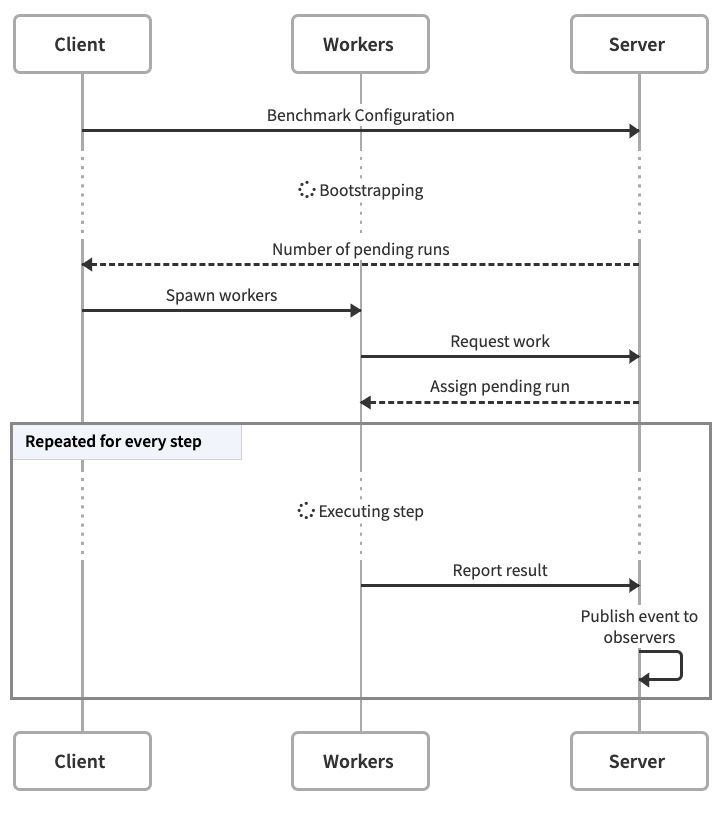
\includegraphics[width=\textwidth]{assets/pics/workflow-swimlane.png}
    }
    \caption{Benchmarking workflow}
    \label{fig:swimlane}
\end{figure}

Figure \ref{fig:swimlane} presents the steps and interactions taken by each actors, namely the Client, Workers, and Server.
Aside from the already defined Workers and Server in Section \ref{sec:impl.architecture} above, Client represents the actual user interfacing with \OurBenchmarkingTool.
Note that the figure assumes the server is already started.

First, the client uses the bootstrapper to read the configuration and then send a bootstrap event to the server.
This event includes the needed information for the server to also set up the database schema.
Then the server replies its readiness to the client.
After that, the client uses the manager to spawn workers.
This is the end of the interaction needed by the user.

Then, after being scheduled by the job scheduling system used by the manager, each worker request the context for its assigned run identifier to the server.
The server replies with the context.
This includes things such as the tool and its configuration, the input instance, resource limits, etc.

Then come the main computation represented as run steps.
Each steps is executed sequentially.
After execution of the step, typically the worker will report the result to the server which in turn publish that event to observers.
Any observers listening to the event will execute its work, often time this means inserting data to the database. After there is no more run step to execute, the worker sends a finish event to the server and terminates.

As soon as soon as the bootstrapping is done, analysis can be executed from the available data in database.
This allows the flexibility of doing either on-demand analysis or live analysis.


\subsection{Benchmarking Model}

\First~decided to define the data as relational model of SQL, as opposed to nonrelational model of NoSQL.
The reason is because SQL provides an easy and fast interface for querying and aggregating data, tasks that occur often when analyzing benchmark results.
The benchmarking process itself can be defined nicely into structured relations, centering on benchmark runs.

\begin{figure}
    \centering
    \ifdraft{
        \dummyfig{assets/pics/erd.png}
    }{
        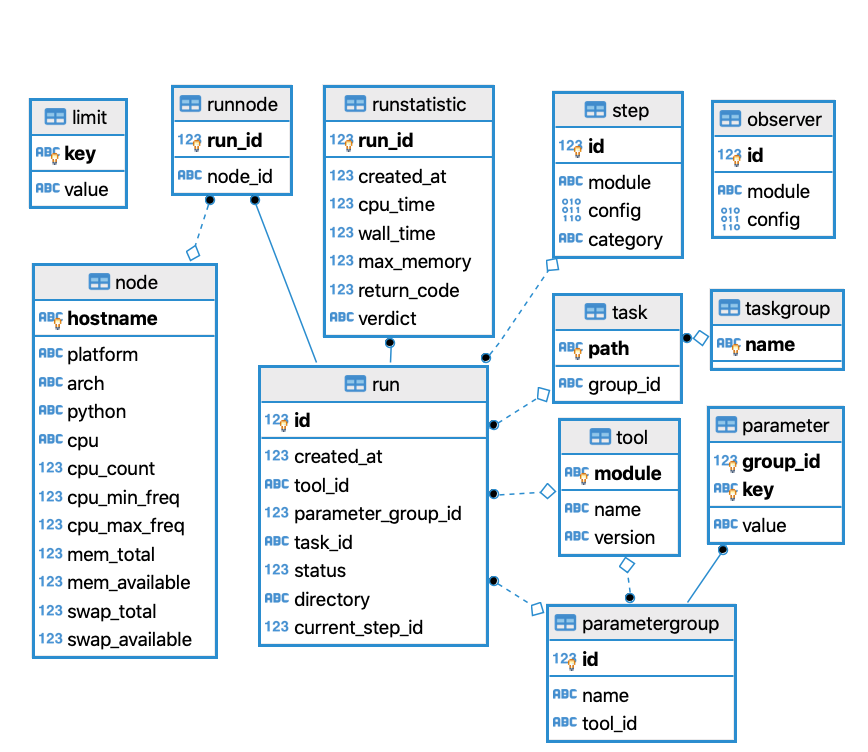
\includegraphics[width=\textwidth]{assets/pics/erd.png}
    }
    \caption{Entity-relationship diagram of \OurBenchmarkingTool's model}
    \label{fig:erd}
\end{figure}

The benchmarking process is modeled as in the entity-relationship diagram (ERD) shown in Figure \ref{fig:erd}.
The database stores every configuration defined to support reproducibility.
Among the core entities are \textsc{run}, \textsc{tool}, \textsc{parameter}, \textsc{limit}, \textsc{step}, \textsc{observer}, and \textsc{task}.
Some entities like \textsc{parameter} and \textsc{task} are grouped to another intermediate many-to-many entity, that is \textsc{parameterGroup} and \textsc{taskGroup}.
It can be seen that the relationship centers around the \textsc{run} entity.

Other modules, like the ones used as steps, can then register its own model to store its data, such as \textsc{runstatistic} (by the executor module) or \textsc{runnode} (by the system information collector module).
This supports separation of concern and encapsulation of the module.
User can use community-created module without having to consider its data model.

In fact, it is also possible to move all the data that is normally stored in the filesystem into the SQL table.
Many SQL database engine provides a BLOB data type to store binary data.
For example, \textsc{SQLite} even has an archiving tool called \code{sqlar}\footlink{https://www.sqlite.org/sqlar} that use the database as storage just like a ZIP archive.
This allow the database to store everything needed to reproduce the benchmark.
But \first~decided not to do it to make debugging runs easier, a task which also occur surprisingly often alongside benchmarking.

\section{Implementation}
\label{sec:impl.impl}

\newstyle{
This section presents details regarding the implementation of \OurBenchmarkingTool.
It will be organized by the components of the benchmarking tool.
The complete implementation source code is attached in the appendix.
It is also available as Git repository: \href{https://github.com/rkkautsar/reprobench}{\code{https://github.com/rkkautsar/reprobench}} and pypi package: \href{https://pypi.org/project/reprobench/}{\code{https://pypi.org/project/reprobench/}}.
}

\subsection{Development Environment}

\First~choose Python as the main programming language.
Specifically, Python 3 is used as its predecessor Python 2 will meet its end of the line and not be supported anymore in 2020.
It is a widely available language with huge community.
Python also has good interopability with C and C++, it's relatively easy to write wrappers of C libraries to Python.
That said, there is a huge collection of publicly available python packages in the Python Package Index (pypi)\footlink{https://pypi.org/} readily installable through \code{pip} tool, which often distributed alongside Python.
This allows for rapid software development by reducing common implementation.

Being an interpreter and not a compiled language, Python is relatively slow.
For this project, speed can be sacrificed in place of developer experience.
Most of the CPU usage will be used by the benchmarked program anyway, so the development speed is arguably more important.

\First~use a combination of \textsc{pyenv}\footlink{https://github.com/pyenv/pyenv} and \textsc{poetry}\footlink{https://github.com/sdispater/poetry} to manage dependencies and package publishing.
With \textsc{pyenv}, it is easy to switch between specific versions of Python and also pin a project to use specific version of Python.
This allow reproducible development environment across machines without influence from other projects using different Python version.
Additionally, testing if the software works under specific version of Python is a trivial task.
\textsc{poetry} on the other hand, manages the dependencies in a virtual environment with version locking.
This allows separate, reproducible dependencies across projects.
\textsc{poetry} also provide simple API to package and publish the project to pypi.
Under a UNIX system, setting up both tools is easy and works without superuser privilege, as seen in \lst~\ref{lst:impl.setup.pyenv.poetry}.

\begin{listing}
    \begin{minted}{bash}
$ curl https://pyenv.run | bash
$ pyenv install "3.7.2"
$ pyenv global "3.7.2"
$ pip install poetry
    \end{minted}
    \caption{Setting up \textsc{pyenv} and \textsc{poetry}}
    \label{lst:impl.setup.pyenv.poetry}
\end{listing}

The source code is organized by the Git version control and made publicly available in GitHub.
This allows others to freely contribute to the project and also encourage them to also make their modules open-source.
Additionally, the source code is licensed under the MIT License to allow permissive usage.

\subsection{Project Structure}
\label{sec:impl.structure}

The source code organization and their brief descriptions is listed below:
\begin{itemize}
    \item \emph{examples/}\\
          This directory provides a collection of working usage benchmark examples demonstrating various features of the benchmarking tool.

    \item \emph{pyproject.toml}\\
          Configuration file describing the various dependencies used and the packaging options used for publishing purposes.

    \item \emph{reprobench/console/}\\
          This directory consists of the implementations of the command line interface (CLI), including the \code{reprobench} root command and related setup for the sub-commands.

    \item \emph{reprobench/core/}\\
          The core implementation of \OurBenchmarkingTool~is organized in this directory.
          This includes generic classes, database models, and implementation for the worker, server, bootstrapper, and analyzer components.

    \item \emph{reprobench/executors/}\\
          Implementations of the special run step doing the actual execution and monitoring of the tools and its input.
          This includes the accompanying observer, its database model and related events.

    \item \emph{reprobench/managers/}\\
          Implementations of the manager component and its CLI sub-commands under the \code{reprobench manage} sub-command, e.g. \code{reprobench manage local} or \code{reprobench manage slurm}.
          In the future, it is preferable for each manager to be separated into its own package.

    \item \emph{reprobench/statistics/}\\
          This directory consists of reference implementations of the analysis step modules.
          It is encouraged to implement analysis steps as separate packages and only put the most general ones in the main project.

    \item \emph{reprobench/task\_sources/}\\
          This directory consists of various implementation for extracting tasks from the configuration.
          Currently, this includes local filesystem sourced tasks, URL-based remote sourced tasks, and Digital Object Identifier (DOI) sourced tasks.

    \item \emph{reprobench/tools/}\\
          This directory implements some base classes to be extended for writing tool interfaces.
          It is also possible in the future to allow tools to be defined only from the configuration, further lowering the barrier for using this benchmarking tool.
          Writing tool interface is discussed in Section \ref{sec:impl.tools}.

    \item \emph{reprobench/utils.py}\\
          This file consists of various small utilities commonly used by the implementation.


\end{itemize}


\subsection{Configuration}

\begin{listing}
    \inputminted{yaml}{assets/listings/pseudocodes/config.yml}
    \caption{Example of \OurBenchmarkingTool~configuration file}
    \label{lst:impl.config.example}
\end{listing}

Configuration for a benchmark is done using a YAML file, provided to the bootstrapper.
An example configuration file is shown in \lst~\ref{lst:impl.config.example}.
\First~choose YAML file over other format because of it is readable and easy to edit by hand.
It is also widely adopted and implemented in various programming languages.
\First~also considered to use XML or JSON but find both to be harder to edit by hand.

``YAML Ain’t Markup Language'', recursively abbreviated to YAML, is a data serialization language designed to be human-friendly, portable between programming languages, and easy to use for every tasks \citep{ben2005yaml}.
While it's easy to understand at a glance, it has an arguably complex specification allowing for various use cases.
Avoiding its complexity, \first~choose to use \textsc{StrictYAML}\footlink{https://github.com/crdoconnor/strictyaml}, a relatively simple implementation of a small subset of the YAML specification.
\textsc{StrictYAML} also allows definition of a schema to provide type-safe parsing.
The schema for \OurBenchmarkingTool~configuration file is defined in \emph{reprobench/core/schema.py}.


\subsection{Module}

To enable high extensibility, many components of \OurBenchmarkingTool~is defined in a modular, reusable Python \emph{modules}.
What \first~define as a module is in fact just a Python class that can be imported by path strings.
For example, the path string \mintinline{python}{"my_package.my_folder.my_file.MyClass"} references the class \code{MyClass} in \emph{my\_folder/my\_file.py} (or \emph{my\_folder/my\_file/\_\_init\_\_.py}) file in the Python package \code{my\_package}.
This allows \OurBenchmarkingTool~to flexibly import user defined code, either it's in the working directory or installed through \code{pip}.


\subsection{Server}

\begin{listing}
    \inputminted{python}{assets/listings/pseudocodes/server.py}
    \caption{Pseudo-code of the server component}
    \label{lst:impl.server}
    % \captionof{listing}{Pseudo-code of the server component \label{lst:impl.server}}
\end{listing}

Pseudo-code for the server implementation is given in \lst~\ref{lst:impl.server}.
In short, the server is implemented in three main phases.
The first phase is setting up the database and sockets.
Then the server waits for a \textsc{bootstrap} event from the client, as mentioned in Section \ref{sec:impl.design} earlier.
As soon as the database is bootstrapped, the server query the needed observers and register the respective modules.
Finally, the server spawn `greenlets' of the observers and its own loop method and waited for them to terminate.

\textsc{greenlet}\footlink{https://github.com/python-greenlet/greenlet} is a Python package that provides the use of `greenlets'.
A greenlet is a lightweight pseudo-thread useful for concurrent programming.
In contrast with implicit context switching of native OS-level threads, greenlet explicitly context switches.
In short, it's a way of programmatically jump from one code frame to another, allowing thread-like behavior with minimal runtime overhead.
This fits to \firstposs~need of concurrency for controlling the flow in the server.

On the first phase, an \textsc{SQLite} database are initiated in the given output path.
\First~choose to use SQLite because it is most of the time already available in various platforms.
Even when it is not available, it can be installed easily with pre-compiled binaries or as a single-file C source code.
It is also works on a single file database, allowing easy distribution for reproducibility.
The \textsc{SQLite} database is opened in \emph{Write-ahead logging} mode to better handle concurrency.

Two socket connections are also prepared in this phase.
The official Python bindings for \O MQ, \textsc{pyzmq}\footlink{https://github.com/zeromq/pyzmq} is used to setup the related sockets.
These two sockets are \textsc{router} and \textsc{pub} as discussed in Section \ref{sec:impl.messaging}.
On one hand, the \textsc{router} socket acts as a `front-end' gateway and interacts with clients.
On the other hand, the \textsc{pub} socket interacts with the observer greenlets and acts as the `back-end' gateway.

Then the server waits for a bootstrap event from the client.
Events are encoded with \textsc{MessagePack}\footlink{https://msgpack.org/} binary serialization format to minimize the amount of data transferred.
It enters a loop waiting for the specific \textsc{bootstrap} event.
After receiving this event, the server prepare the database schema with the payload from the event.
Then the server loads the observer modules.
The list of observer modules is extracted from the database, inserted from the earlier bootstrapping process.

The server spawns greenlets of the observers and its own loop method.
The loop method waits for every event received in the front-end socket and forward it to the back-end socket, allowing the observers to act accordingly.

The run step (explained in Section \ref{sec:impl.workers}) is usually accompanied by an observer.
An observer is a class extending \mintinline{python}{class Observer} imported from \code{reprobench.core.base}.
Since observers live in the server process, naturally they mostly deal with the database.
This does not only include inserting data to the database, implementing notifications to e-mail or even to messaging services like Slack or Telegram is also possible.

\begin{listing}
    \inputminted[firstline=7,lastline=13]{python}{assets/listings/reprobench/reprobench/executors/base.py}
    \caption{An example observer used by the executor step}
    \label{lst:impl.observer}
\end{listing}

One example can be seen in \lst~\ref{lst:impl.observer}, showing the observer accompanying the executor step.
The most basic implementation of an observer includes defining the events it subscribes to in the \mintinline{python}{SUBSCRIBED_EVENTS} attribute and defining the \mintinline{python}{def handle_event(cls, ...)} class method.
This observer is stated in the configuration file as a module.
Additionally, there is also a single core observer that is always included regardless of the configuration.
It is defined as \mintinline{python}{class CoreObserver(Observer)} in \emph{reprobench/core/observers.py}.

\subsection{Bootstrapper}

The bootstrapper component receives the configuration file and prepare the execution environment accordingly.
There is two bootstrapping process that take place.
Both are defined in \emph{reprobench/core/bootstrap/} as \mintinline{python}{def bootstrap_client(...)} in \code{client.py} and \mintinline{python}{def bootstrap_server(...)} in \code{server.py}.
The client-side will prepare the execution environment, after that it passes the required information to the server-side.
The server-side will then prepare for the data-related things such as the database schema.

Additionally, it is also possible to update the configuration---mostly data-related---of an in-progress benchmark.
This is also done by the bootstrapper, but the related code is contained in \emph{reprobench/core/update.py}.
In essence, update is executed when the server detected that the database is in fact already bootstrapped.
This allow addition of tools, parameters, or tasks to an already bootstrapped benchmark, ensuring the workflow is as flexible and as natural as possible.

\subsection{Manager}

Manager manages the formation and termination of workers.
It acts on top of the existing job scheduling system or manage its own queue system.
A manager implementation extends \mintinline{python}{class BaseManager} defined in \emph{reprobench/managers/base.py}.
\lst~\ref{lst:impl.manager} shows this base class and the base implementation.

\begin{listing}
    \inputminted[firstline=7,lastline=34]{python}{assets/listings/reprobench/reprobench/managers/base.py}
    \caption{The BaseManager class}
    \label{lst:impl.manager}
\end{listing}

The main method can be seen in \mintinline{python}{def run(self)}.
First it calls the optional \mintinline{python}{def prepare(self)} method.
Then it requests and stores the list of pending runs from the server.
Finally it spawn the workers and wait for them to be terminated.
Currently, two managers are implemented, namely the local manager and the \textsc{slurm} manager.

The local manager as the most basic manager which implements its own scheduling system.
This is typically used when the benchmarking tool is used---for quick benchmarking or testing, for example---outside the HPC cluster system.
This manager maintains a process pool whose number of processes can be defined or defaults to the number of available cores.
This pool of process then gets the job from the pending runs and spawn a worker exclusively for that job.
This repeats until there is no more pending runs.

The \textsc{slurm} manager works in the \textsc{slurm} cluster system\footlink{https://www.schedmd.com/} and also acts as a reference implementation for other potential managers.
The implementation of this manager is straightforward.
It submits the pending runs as a job array of the worker process with the \code{sbatch} command and cancel them when requested with the \code{scancel} command.

\subsection{Workers}
\label{sec:impl.workers}

\begin{listing}
    \inputminted{python}{assets/listings/pseudocodes/worker.py}
    \caption{Pseudo-code of the worker component}
    \label{lst:impl.worker}
\end{listing}

The worker is an implementation-agnostic process whose only purpose is to execute the run steps on top of the benchmark run.
The pseudo-code of the implementation can be seen in \lst~\ref{lst:impl.worker}.
First, it reports its existence to the server and requests for information (or context) regarding its assigned run.
Then it creates a context object to be passed to steps, and executes them one by one sequentially.
When it finishes executing all the steps, it reports its completion and terminates.

A step is implemented as a subclass of \mintinline{python}{class Step} in \emph{reprobench/core/base.py}.
This base class defines only two class methods, \mintinline{python}{def register(cls, config)} and \mintinline{python}{def execute(cls, context, config)}.
The register method is called on bootstrap phase and the execute method is called by the workers.
Typically, the register method contains a database schema creation routine executed in the server-side.

Steps are used in two benchmarking phase, that is the running phase and the analysis phase.
These are differentiated in the configuration file under the \code{steps} key.
One such example of a run step---a step executed in the running phase---is the executor.
While an example of an analysis step---a step executed in the analysis phase---is spreadsheet generation summarizing statistics from the database.

\subsection{Tools}
\label{sec:impl.tools}

To allow the benchmarking of any tools, there needs to be a common interface for interaction between \OurBenchmarkingTool~and the tool.
Thus, benchmarking a tool in \OurBenchmarkingTool~also involves writing the respective interface module.
A tool interface subclasses the base \mintinline{python}{class Tool} in \emph{reprobench/core/base.py}.
Typically the user will not directly subclass this abstract class but instead subclass the more specific base class like the \mintinline{python}{class ExecutableTool(Tool)} defined in \emph{reprobench/tools/executable.py}.

\begin{listing}
    \inputminted[firstline=12]{python}{assets/listings/reprobench/examples/sat/tools/glucose.py}
    \caption{Example tool interface implementation}
    \label{lst:impl.tool.example}
\end{listing}

\lst~\ref{lst:impl.tool.example} presents an example of one such tool interface.
This module defines its setup routine, involving downloading from specific URL and building with the GNU \code{make} tool.
The \mintinline{python}{class ExecutableTool(Tool)} already takes care of setting the arguments and running the actual tool.
This makes writing a tool interface easy with minimum effort.
It is encouraged to create various abstractions from the base \mintinline{python}{class Tool} to further minimize the effort.

Tools can be configured to use various parameters specified in the configuration file, as seen in \lst~\ref{lst:impl.config.example}.
\OurBenchmarkingTool~supports defining parameter as ranges, that is by using an integer range syntax such as \code{1..10} or using YAML list syntax.
Additionally, it also supports defining parameter range through a parameter configuration space (.pcs) file, allowing easy integration for tools already using this file for configuration.
These parameters are processed by the tool interface and turn into arguments, for example.


\subsection{Task Sources}

To support achieving \(\bm{R_2}\) reproducibility, benchmark instances is encouraged to be sourced from remote location instead of local file system.
For example, as seen in the example configuration in \lst~\ref{lst:impl.config.example} it can be sourced from specified URL.
Of course it is still possible to use files in the local system but the use is discouraged as it will make the benchmarking process less portable and less reproducible.

Task source implementation extends \mintinline{python}{class BaseTaskSource} defined in \emph{reprobench/task\_sources/base.py}.
This base class contains a single \mintinline{python}{def setup(self)} method which returns a list of `tasks' and an init function.
A task source class will be initialized by its defined configuration and then the setup method is then executed to get the list of tasks.

As mentioned briefly in Section \ref{sec:impl.structure}, currently there are three implementation of this task source, namely local-based, URL-based, and DOI-based.
The DOI-based task source extends the URL-based task source which in turn also an extension of the local-based task source.
Note that the DOI-based task source only works with DOIs from Zenodo\footlink{http://zenodo.org}, but it is trivial to add support for more sources.

The URL-based task source allows one to specify a URL for downloading the benchmark instances.
Combined with the automated download and setup of tools, one can just share the configuration file without having to worry about the tools or the benchmark instances.
Thus it is two less thing to worry about for achieving \(\bm{R_1}\) reproducibility.


\subsection{Command Line Interface}

User interacts with \OurBenchmarkingTool~through a command line interface (CLI).
It is also possible to create a graphical user interface or a web-based one, but \first~leave it for future works.
\OurBenchmarkingTool~CLI is structured with sub-commands, each having their own arguments and options.
\tab~\ref{tab:cli} shows description of each commands with its options and arguments.
These description can also be accessed behind the \code{--help} option.

\begin{table}
    \begin{threeparttable}
        \begin{adjustbox}{max width=\textwidth}
            \begin{tabular}{llp{5cm}l}
                \textbf{Command} & \textbf{Option/Argument}\tnote{$\alpha$}                                     & \textbf{Description}                              & \textbf{Default value}       \\
                \toprule

                \multirow{2}{*}{\code{reprobench}}
                                 & \multicolumn{3}{l}{\textit{Root command of \OurBenchmarkingTool}}                                                                                               \\*
                                 & \code{--version}                                                             & Prints the version                                &                              \\*
                \midrule

                \multirow{3}{*}{\code{\dots~server}}
                                 & \multicolumn{3}{l}{\textit{Start the server}}                                                                                                                   \\*
                                 & \code{-d, --output-dir}                                                      & Set output directory, e.g. for the database file  & ./output                     \\*
                                 & \code{-a, --address}                                                         & Address to listen to                              & tcp://127.0.0.1:31313        \\*
                \midrule

                \multirow{5}{*}{\code{\dots~bootstrap}}
                                 & \multicolumn{3}{l}{\textit{Execute the bootstrapping process}}                                                                                                  \\*
                                 & \code{[config]}                                                              & Configuration file to use                         & ./benchmark.yml              \\*                                                                                               \\*
                                 & \code{-r, --repeat}                                                          & Set run repetition                                & 1                            \\*
                                 & \code{-d, --output-dir}                                                      & Set output directory, e.g.for organizing the runs & ./output                     \\*
                                 & \code{-a, --address}                                                         & Server address                                    & tcp://127.0.0.1:31313        \\*
                \midrule

                \multirow{7}{*}{\code{\dots~manage}}
                                 & \multicolumn{3}{l}{\textit{Use the selected manager to manage the workers.}}                                                                                    \\*
                                 & \code{[manager]}                                                             & local or slurm                                    &                              \\*                                                                                               \\*
                                 & \code{[command]}                                                             & run or stop\tnote{$\beta$}                        &                              \\*                                                                                               \\*
                                 & \code{[config]}\tnote{$\beta$}                                               & Configuration file to use                         &                              \\*                                                                                               \\*
                                 & \code{-w, --num-workers}\tnote{$\gamma$}                                     & Set the number of worker process pool             & \em{depends}\tnote{$\delta$} \\*
                                 & \code{-d, --output-dir}                                                      & Set output directory, e.g.for organizing the runs & ./output                     \\*
                                 & \code{-a, --address}                                                         & Server address                                    & tcp://127.0.0.1:31313        \\*
                \midrule

                \multirow{3}{*}{\code{\dots~worker}}
                                 & \multicolumn{3}{l}{\textit{Start a worker manually}}                                                                                                            \\*
                                 & \code{[run\_id]}                                                             & Run identifier assigned to the worker             &                              \\*
                                 & \code{-a, --address}                                                         & Server address                                    & tcp://127.0.0.1:31313        \\*
                \midrule

                \multirow{3}{*}{\code{\dots~status}}
                                 & \multicolumn{3}{l}{\textit{Monitor the benchmarking progress}}                                                                                                  \\*
                                 & \code{-d, --output-dir}                                                      & Output directory containing the database          & ./output                     \\*
                                 & \code{-n, --interval}                                                        & Polling interval in seconds                       & 2                            \\*
                \midrule

                \multirow{2}{*}{\code{\dots~analyze}}
                                 & \multicolumn{3}{l}{\textit{Run the analysis step	}}                                                                                                              \\*
                                 & \code{-d, --output-dir}                                                      & Output directory containing the database          & ./output                     \\*
                \bottomrule
            \end{tabular}
        \end{adjustbox}

        \begin{tablenotes}
            \footnotesize
            \item[$\alpha$] Arguments are denoted as \code{[argument]}.
            \item[$\beta$] Slurm manager only.
            \item[$\gamma$] Local manager only.
            \item[$\delta$] Number of available (virtual) cores.
        \end{tablenotes}

        \caption{\OurBenchmarkingTool~CLI commands}
        \label{tab:cli}
    \end{threeparttable}
\end{table}
\chapter{\chEvaluation}
\label{ch:evaluation}

This chapter presents several evaluation regarding the implementation of \OurBenchmarkingTool~and its position relative to other benchmarking tools mentioned in \Cref{ch:existing}.
First, an example usage scenario is given in \Cref{sec:eval.scenario} to give an overview of how \OurBenchmarkingTool~can be used from setting up, running the benchmark, until the analysis step.
\Cref{sec:eval.messaging} gives a detailed look to the performance and implications of the implemented messaging mechanism.
A measurement of the resource usage of the implementation is then given in \Cref{sec:eval.resource}.
Last but not least, comparisons to other mentioned benchmarking tools is discussed in \Cref{sec:eval.comparison} based on a breakdown of the requirements from \Cref{sec:idealBenchmarkingTool}.

\section{Example Usage Scenario}
\label{sec:eval.scenario}

This section describe an example benchmarking workflow using \OurBenchmarkingTool.
Each step needed from setting up to analyzing the result is explained.

\subsection{Benchmark Setup}

The configuration for this benchmarking scenario is publicly available as a GitHub repository: \href{https://github.com/rkkautsar/benchmark-demo-sat}{\code{https://github.com/rkkautsar/benchmark-demo-sat}}.
The configuration is the same as in \lst~\ref{lst:impl.config.example}.
This benchmark is \(\bm{R_1}\) reproducible in UNIX machines.
The tools and tasks are downloaded from the internet and set up programmatically.

For this scenario, the benchmarking is done in three environment.
Computation is done in a \textsc{slurm} cluster system of TU Dresden, Taurus.
Taurus sports 2\,179 nodes with a total of 41\,468 cores.
A typical node used for the computation has an Intel(R) Xeon(R) CPU E5-2690 @ 2.90GHz.
Data collection is done in a VPS physically located in Paris, France.
This is a small € 2.40 virtual instance sporting an Intel(R) Atom(TM) CPU C3955 @ 2.10GHz and 1 GB of RAM.
For future reference, \first~refer to the IP bound for this VPS as \code{168.8.8.8}.
Finally, the analysis is done in a personal machine with a Intel Core i5 CPU @ 1.8 GHz.
This is not necessary but in this scenario it is needed to execute an analysis in a Jupyter notebook.

\subsection{Installation}

As noted in Chapter \ref{ch:implementation}, \OurBenchmarkingTool~is distributed through the Python's standard pypi.
There are various specific extra dependencies that also need to be installed depending on what the \OurBenchmarkingTool~will be doing in the system.
This is taken care using the `extras' dependencies specification of the package.

\begin{listing}
	\begin{minted}{bash}
client $ pip install reprobench[client,sysinfo,psmon]
server $ pip install reprobench[server,pcs]
personal $ pip install reprobench[analytics]
    \end{minted}
	\caption{Installing \OurBenchmarkingTool~in various environment}
	\label{lst:eval.install}
\end{listing}

For example, one might want to set up to three different environment.
These are the client-side for running the computation, server-side for collecting the data, and their own personal machine for analysis.
\Cref{lst:eval.install} shows how the installation can be done for each environment.

Additionally, Python's \code{virtualenv} is used in the server-side to contain the dependencies.
In client-side, a Miniconda\footlink{https://docs.conda.io/en/latest/miniconda.html} environment is used instead.
Finally, a Jupyter\footlink{https://jupyter.org/} and IPython kernel is installed for running the analysis.
Also, the repository is cloned to each environment.

\subsection{Running the Benchmark}

\begin{listing}
	\begin{minted}{text}
server $ reprobench server -a tcp://0.0.0.0:31313
client $ reprobench bootstrap -a tcp://168.8.8.8:31313
client $ reprobench manager slurm run -a tcp://168.8.8.8:31313
server $ reprobench status
 74%[#######################        ] 3904/5304 [20:18<21:00,  1.11it/s]
    \end{minted}
	\caption{Running the benchmark}
	\label{lst:eval.running}
\end{listing}

\Cref{lst:eval.running} shows the series of commands executed for running the benchmark.
First, the server process is started and bind a TCP socket at \code{0.0.0.0:31313}.
Note that exposing a port to public like this is not safe per se.
This issue is discussed later in \Cref{ch:conclusion}.

Then the bootstrapping process is started from the client.
Tools and tasks are downloaded first in the client-side before it compiles the information and send it to the server to do its own bootstrapping process.
This whole process may take a while.
In this scenario and the environment listed earlier, it takes about a minute to fully download the tools, tasks, and ready the database.

Last but not least, the \textsc{slurm} manager spawn the workers to do the computation.
This submits a 5,304-sized job array to the job queue, as much as the number of pending runs, which also happen to be the total number of runs in the beginning.
While the worker interacts with the server and do the computation, a \code{reprobench status} command can be used to monitor the progress in real time.
Besides giving reports of the progress, this command also gives an estimate of the remaining time to completion by analyzing the speed of completion.

\subsection{Analysis}

After the benchmarking is completed, the resulting database from the server is obtained for example by using the \code{scp} command such as \mintinline{bash}{scp server:/tmp/benchmark/output/benchmark.db ./output/benchmark.db}.
This database contains all the configuration for this benchmark and can also be shared for others to analyze, validate or even replicate.
The analysis is then executed by running the \code{reprobench analyze} command with the output directory as an argument.

\begin{figure}
	\centering
	% \dummyfig{assets/plots/cactus.pgf}
	\ifdraft{
		\dummyfig{assets/plots/cactus.pgf}
	}{
		\resizebox{\textwidth}{!}{%% Creator: Matplotlib, PGF backend
%%
%% To include the figure in your LaTeX document, write
%%   \input{<filename>.pgf}
%%
%% Make sure the required packages are loaded in your preamble
%%   \usepackage{pgf}
%%
%% Figures using additional raster images can only be included by \input if
%% they are in the same directory as the main LaTeX file. For loading figures
%% from other directories you can use the `import` package
%%   \usepackage{import}
%% and then include the figures with
%%   \import{<path to file>}{<filename>.pgf}
%%
%% Matplotlib used the following preamble
%%   \usepackage{fontspec}
%%   \setmainfont{DejaVuSans.ttf}[Path=/Users/rkkautsar/.pyenv/versions/miniconda3-4.3.30/envs/reprobench/lib/python3.7/site-packages/matplotlib/mpl-data/fonts/ttf/]
%%   \setsansfont{DejaVuSans.ttf}[Path=/Users/rkkautsar/.pyenv/versions/miniconda3-4.3.30/envs/reprobench/lib/python3.7/site-packages/matplotlib/mpl-data/fonts/ttf/]
%%   \setmonofont{DejaVuSansMono.ttf}[Path=/Users/rkkautsar/.pyenv/versions/miniconda3-4.3.30/envs/reprobench/lib/python3.7/site-packages/matplotlib/mpl-data/fonts/ttf/]
%%
\begingroup%
\makeatletter%
\begin{pgfpicture}%
\pgfpathrectangle{\pgfpointorigin}{\pgfqpoint{8.000000in}{6.000000in}}%
\pgfusepath{use as bounding box, clip}%
\begin{pgfscope}%
\pgfsetbuttcap%
\pgfsetmiterjoin%
\definecolor{currentfill}{rgb}{1.000000,1.000000,1.000000}%
\pgfsetfillcolor{currentfill}%
\pgfsetlinewidth{0.000000pt}%
\definecolor{currentstroke}{rgb}{1.000000,1.000000,1.000000}%
\pgfsetstrokecolor{currentstroke}%
\pgfsetdash{}{0pt}%
\pgfpathmoveto{\pgfqpoint{0.000000in}{0.000000in}}%
\pgfpathlineto{\pgfqpoint{8.000000in}{0.000000in}}%
\pgfpathlineto{\pgfqpoint{8.000000in}{6.000000in}}%
\pgfpathlineto{\pgfqpoint{0.000000in}{6.000000in}}%
\pgfpathclose%
\pgfusepath{fill}%
\end{pgfscope}%
\begin{pgfscope}%
\pgfsetbuttcap%
\pgfsetmiterjoin%
\definecolor{currentfill}{rgb}{1.000000,1.000000,1.000000}%
\pgfsetfillcolor{currentfill}%
\pgfsetlinewidth{0.000000pt}%
\definecolor{currentstroke}{rgb}{0.000000,0.000000,0.000000}%
\pgfsetstrokecolor{currentstroke}%
\pgfsetstrokeopacity{0.000000}%
\pgfsetdash{}{0pt}%
\pgfpathmoveto{\pgfqpoint{1.000000in}{0.750000in}}%
\pgfpathlineto{\pgfqpoint{7.200000in}{0.750000in}}%
\pgfpathlineto{\pgfqpoint{7.200000in}{5.280000in}}%
\pgfpathlineto{\pgfqpoint{1.000000in}{5.280000in}}%
\pgfpathclose%
\pgfusepath{fill}%
\end{pgfscope}%
\begin{pgfscope}%
\pgfsetbuttcap%
\pgfsetroundjoin%
\definecolor{currentfill}{rgb}{0.000000,0.000000,0.000000}%
\pgfsetfillcolor{currentfill}%
\pgfsetlinewidth{0.803000pt}%
\definecolor{currentstroke}{rgb}{0.000000,0.000000,0.000000}%
\pgfsetstrokecolor{currentstroke}%
\pgfsetdash{}{0pt}%
\pgfsys@defobject{currentmarker}{\pgfqpoint{0.000000in}{-0.048611in}}{\pgfqpoint{0.000000in}{0.000000in}}{%
\pgfpathmoveto{\pgfqpoint{0.000000in}{0.000000in}}%
\pgfpathlineto{\pgfqpoint{0.000000in}{-0.048611in}}%
\pgfusepath{stroke,fill}%
}%
\begin{pgfscope}%
\pgfsys@transformshift{1.281818in}{0.750000in}%
\pgfsys@useobject{currentmarker}{}%
\end{pgfscope}%
\end{pgfscope}%
\begin{pgfscope}%
\definecolor{textcolor}{rgb}{0.000000,0.000000,0.000000}%
\pgfsetstrokecolor{textcolor}%
\pgfsetfillcolor{textcolor}%
\pgftext[x=1.281818in,y=0.652778in,,top]{\color{textcolor}\rmfamily\fontsize{10.000000}{12.000000}\selectfont 0}%
\end{pgfscope}%
\begin{pgfscope}%
\pgfsetbuttcap%
\pgfsetroundjoin%
\definecolor{currentfill}{rgb}{0.000000,0.000000,0.000000}%
\pgfsetfillcolor{currentfill}%
\pgfsetlinewidth{0.803000pt}%
\definecolor{currentstroke}{rgb}{0.000000,0.000000,0.000000}%
\pgfsetstrokecolor{currentstroke}%
\pgfsetdash{}{0pt}%
\pgfsys@defobject{currentmarker}{\pgfqpoint{0.000000in}{-0.048611in}}{\pgfqpoint{0.000000in}{0.000000in}}{%
\pgfpathmoveto{\pgfqpoint{0.000000in}{0.000000in}}%
\pgfpathlineto{\pgfqpoint{0.000000in}{-0.048611in}}%
\pgfusepath{stroke,fill}%
}%
\begin{pgfscope}%
\pgfsys@transformshift{2.432096in}{0.750000in}%
\pgfsys@useobject{currentmarker}{}%
\end{pgfscope}%
\end{pgfscope}%
\begin{pgfscope}%
\definecolor{textcolor}{rgb}{0.000000,0.000000,0.000000}%
\pgfsetstrokecolor{textcolor}%
\pgfsetfillcolor{textcolor}%
\pgftext[x=2.432096in,y=0.652778in,,top]{\color{textcolor}\rmfamily\fontsize{10.000000}{12.000000}\selectfont 10}%
\end{pgfscope}%
\begin{pgfscope}%
\pgfsetbuttcap%
\pgfsetroundjoin%
\definecolor{currentfill}{rgb}{0.000000,0.000000,0.000000}%
\pgfsetfillcolor{currentfill}%
\pgfsetlinewidth{0.803000pt}%
\definecolor{currentstroke}{rgb}{0.000000,0.000000,0.000000}%
\pgfsetstrokecolor{currentstroke}%
\pgfsetdash{}{0pt}%
\pgfsys@defobject{currentmarker}{\pgfqpoint{0.000000in}{-0.048611in}}{\pgfqpoint{0.000000in}{0.000000in}}{%
\pgfpathmoveto{\pgfqpoint{0.000000in}{0.000000in}}%
\pgfpathlineto{\pgfqpoint{0.000000in}{-0.048611in}}%
\pgfusepath{stroke,fill}%
}%
\begin{pgfscope}%
\pgfsys@transformshift{3.582375in}{0.750000in}%
\pgfsys@useobject{currentmarker}{}%
\end{pgfscope}%
\end{pgfscope}%
\begin{pgfscope}%
\definecolor{textcolor}{rgb}{0.000000,0.000000,0.000000}%
\pgfsetstrokecolor{textcolor}%
\pgfsetfillcolor{textcolor}%
\pgftext[x=3.582375in,y=0.652778in,,top]{\color{textcolor}\rmfamily\fontsize{10.000000}{12.000000}\selectfont 20}%
\end{pgfscope}%
\begin{pgfscope}%
\pgfsetbuttcap%
\pgfsetroundjoin%
\definecolor{currentfill}{rgb}{0.000000,0.000000,0.000000}%
\pgfsetfillcolor{currentfill}%
\pgfsetlinewidth{0.803000pt}%
\definecolor{currentstroke}{rgb}{0.000000,0.000000,0.000000}%
\pgfsetstrokecolor{currentstroke}%
\pgfsetdash{}{0pt}%
\pgfsys@defobject{currentmarker}{\pgfqpoint{0.000000in}{-0.048611in}}{\pgfqpoint{0.000000in}{0.000000in}}{%
\pgfpathmoveto{\pgfqpoint{0.000000in}{0.000000in}}%
\pgfpathlineto{\pgfqpoint{0.000000in}{-0.048611in}}%
\pgfusepath{stroke,fill}%
}%
\begin{pgfscope}%
\pgfsys@transformshift{4.732653in}{0.750000in}%
\pgfsys@useobject{currentmarker}{}%
\end{pgfscope}%
\end{pgfscope}%
\begin{pgfscope}%
\definecolor{textcolor}{rgb}{0.000000,0.000000,0.000000}%
\pgfsetstrokecolor{textcolor}%
\pgfsetfillcolor{textcolor}%
\pgftext[x=4.732653in,y=0.652778in,,top]{\color{textcolor}\rmfamily\fontsize{10.000000}{12.000000}\selectfont 30}%
\end{pgfscope}%
\begin{pgfscope}%
\pgfsetbuttcap%
\pgfsetroundjoin%
\definecolor{currentfill}{rgb}{0.000000,0.000000,0.000000}%
\pgfsetfillcolor{currentfill}%
\pgfsetlinewidth{0.803000pt}%
\definecolor{currentstroke}{rgb}{0.000000,0.000000,0.000000}%
\pgfsetstrokecolor{currentstroke}%
\pgfsetdash{}{0pt}%
\pgfsys@defobject{currentmarker}{\pgfqpoint{0.000000in}{-0.048611in}}{\pgfqpoint{0.000000in}{0.000000in}}{%
\pgfpathmoveto{\pgfqpoint{0.000000in}{0.000000in}}%
\pgfpathlineto{\pgfqpoint{0.000000in}{-0.048611in}}%
\pgfusepath{stroke,fill}%
}%
\begin{pgfscope}%
\pgfsys@transformshift{5.882931in}{0.750000in}%
\pgfsys@useobject{currentmarker}{}%
\end{pgfscope}%
\end{pgfscope}%
\begin{pgfscope}%
\definecolor{textcolor}{rgb}{0.000000,0.000000,0.000000}%
\pgfsetstrokecolor{textcolor}%
\pgfsetfillcolor{textcolor}%
\pgftext[x=5.882931in,y=0.652778in,,top]{\color{textcolor}\rmfamily\fontsize{10.000000}{12.000000}\selectfont 40}%
\end{pgfscope}%
\begin{pgfscope}%
\pgfsetbuttcap%
\pgfsetroundjoin%
\definecolor{currentfill}{rgb}{0.000000,0.000000,0.000000}%
\pgfsetfillcolor{currentfill}%
\pgfsetlinewidth{0.803000pt}%
\definecolor{currentstroke}{rgb}{0.000000,0.000000,0.000000}%
\pgfsetstrokecolor{currentstroke}%
\pgfsetdash{}{0pt}%
\pgfsys@defobject{currentmarker}{\pgfqpoint{0.000000in}{-0.048611in}}{\pgfqpoint{0.000000in}{0.000000in}}{%
\pgfpathmoveto{\pgfqpoint{0.000000in}{0.000000in}}%
\pgfpathlineto{\pgfqpoint{0.000000in}{-0.048611in}}%
\pgfusepath{stroke,fill}%
}%
\begin{pgfscope}%
\pgfsys@transformshift{7.033210in}{0.750000in}%
\pgfsys@useobject{currentmarker}{}%
\end{pgfscope}%
\end{pgfscope}%
\begin{pgfscope}%
\definecolor{textcolor}{rgb}{0.000000,0.000000,0.000000}%
\pgfsetstrokecolor{textcolor}%
\pgfsetfillcolor{textcolor}%
\pgftext[x=7.033210in,y=0.652778in,,top]{\color{textcolor}\rmfamily\fontsize{10.000000}{12.000000}\selectfont 50}%
\end{pgfscope}%
\begin{pgfscope}%
\definecolor{textcolor}{rgb}{0.000000,0.000000,0.000000}%
\pgfsetstrokecolor{textcolor}%
\pgfsetfillcolor{textcolor}%
\pgftext[x=4.100000in,y=0.462809in,,top]{\color{textcolor}\rmfamily\fontsize{10.000000}{12.000000}\selectfont Instance solved}%
\end{pgfscope}%
\begin{pgfscope}%
\pgfsetbuttcap%
\pgfsetroundjoin%
\definecolor{currentfill}{rgb}{0.000000,0.000000,0.000000}%
\pgfsetfillcolor{currentfill}%
\pgfsetlinewidth{0.803000pt}%
\definecolor{currentstroke}{rgb}{0.000000,0.000000,0.000000}%
\pgfsetstrokecolor{currentstroke}%
\pgfsetdash{}{0pt}%
\pgfsys@defobject{currentmarker}{\pgfqpoint{-0.048611in}{0.000000in}}{\pgfqpoint{0.000000in}{0.000000in}}{%
\pgfpathmoveto{\pgfqpoint{0.000000in}{0.000000in}}%
\pgfpathlineto{\pgfqpoint{-0.048611in}{0.000000in}}%
\pgfusepath{stroke,fill}%
}%
\begin{pgfscope}%
\pgfsys@transformshift{1.000000in}{0.904251in}%
\pgfsys@useobject{currentmarker}{}%
\end{pgfscope}%
\end{pgfscope}%
\begin{pgfscope}%
\definecolor{textcolor}{rgb}{0.000000,0.000000,0.000000}%
\pgfsetstrokecolor{textcolor}%
\pgfsetfillcolor{textcolor}%
\pgftext[x=0.814412in,y=0.851489in,left,base]{\color{textcolor}\rmfamily\fontsize{10.000000}{12.000000}\selectfont 0}%
\end{pgfscope}%
\begin{pgfscope}%
\pgfsetbuttcap%
\pgfsetroundjoin%
\definecolor{currentfill}{rgb}{0.000000,0.000000,0.000000}%
\pgfsetfillcolor{currentfill}%
\pgfsetlinewidth{0.803000pt}%
\definecolor{currentstroke}{rgb}{0.000000,0.000000,0.000000}%
\pgfsetstrokecolor{currentstroke}%
\pgfsetdash{}{0pt}%
\pgfsys@defobject{currentmarker}{\pgfqpoint{-0.048611in}{0.000000in}}{\pgfqpoint{0.000000in}{0.000000in}}{%
\pgfpathmoveto{\pgfqpoint{0.000000in}{0.000000in}}%
\pgfpathlineto{\pgfqpoint{-0.048611in}{0.000000in}}%
\pgfusepath{stroke,fill}%
}%
\begin{pgfscope}%
\pgfsys@transformshift{1.000000in}{1.546907in}%
\pgfsys@useobject{currentmarker}{}%
\end{pgfscope}%
\end{pgfscope}%
\begin{pgfscope}%
\definecolor{textcolor}{rgb}{0.000000,0.000000,0.000000}%
\pgfsetstrokecolor{textcolor}%
\pgfsetfillcolor{textcolor}%
\pgftext[x=0.814412in,y=1.494145in,left,base]{\color{textcolor}\rmfamily\fontsize{10.000000}{12.000000}\selectfont 2}%
\end{pgfscope}%
\begin{pgfscope}%
\pgfsetbuttcap%
\pgfsetroundjoin%
\definecolor{currentfill}{rgb}{0.000000,0.000000,0.000000}%
\pgfsetfillcolor{currentfill}%
\pgfsetlinewidth{0.803000pt}%
\definecolor{currentstroke}{rgb}{0.000000,0.000000,0.000000}%
\pgfsetstrokecolor{currentstroke}%
\pgfsetdash{}{0pt}%
\pgfsys@defobject{currentmarker}{\pgfqpoint{-0.048611in}{0.000000in}}{\pgfqpoint{0.000000in}{0.000000in}}{%
\pgfpathmoveto{\pgfqpoint{0.000000in}{0.000000in}}%
\pgfpathlineto{\pgfqpoint{-0.048611in}{0.000000in}}%
\pgfusepath{stroke,fill}%
}%
\begin{pgfscope}%
\pgfsys@transformshift{1.000000in}{2.189562in}%
\pgfsys@useobject{currentmarker}{}%
\end{pgfscope}%
\end{pgfscope}%
\begin{pgfscope}%
\definecolor{textcolor}{rgb}{0.000000,0.000000,0.000000}%
\pgfsetstrokecolor{textcolor}%
\pgfsetfillcolor{textcolor}%
\pgftext[x=0.814412in,y=2.136801in,left,base]{\color{textcolor}\rmfamily\fontsize{10.000000}{12.000000}\selectfont 4}%
\end{pgfscope}%
\begin{pgfscope}%
\pgfsetbuttcap%
\pgfsetroundjoin%
\definecolor{currentfill}{rgb}{0.000000,0.000000,0.000000}%
\pgfsetfillcolor{currentfill}%
\pgfsetlinewidth{0.803000pt}%
\definecolor{currentstroke}{rgb}{0.000000,0.000000,0.000000}%
\pgfsetstrokecolor{currentstroke}%
\pgfsetdash{}{0pt}%
\pgfsys@defobject{currentmarker}{\pgfqpoint{-0.048611in}{0.000000in}}{\pgfqpoint{0.000000in}{0.000000in}}{%
\pgfpathmoveto{\pgfqpoint{0.000000in}{0.000000in}}%
\pgfpathlineto{\pgfqpoint{-0.048611in}{0.000000in}}%
\pgfusepath{stroke,fill}%
}%
\begin{pgfscope}%
\pgfsys@transformshift{1.000000in}{2.832218in}%
\pgfsys@useobject{currentmarker}{}%
\end{pgfscope}%
\end{pgfscope}%
\begin{pgfscope}%
\definecolor{textcolor}{rgb}{0.000000,0.000000,0.000000}%
\pgfsetstrokecolor{textcolor}%
\pgfsetfillcolor{textcolor}%
\pgftext[x=0.814412in,y=2.779457in,left,base]{\color{textcolor}\rmfamily\fontsize{10.000000}{12.000000}\selectfont 6}%
\end{pgfscope}%
\begin{pgfscope}%
\pgfsetbuttcap%
\pgfsetroundjoin%
\definecolor{currentfill}{rgb}{0.000000,0.000000,0.000000}%
\pgfsetfillcolor{currentfill}%
\pgfsetlinewidth{0.803000pt}%
\definecolor{currentstroke}{rgb}{0.000000,0.000000,0.000000}%
\pgfsetstrokecolor{currentstroke}%
\pgfsetdash{}{0pt}%
\pgfsys@defobject{currentmarker}{\pgfqpoint{-0.048611in}{0.000000in}}{\pgfqpoint{0.000000in}{0.000000in}}{%
\pgfpathmoveto{\pgfqpoint{0.000000in}{0.000000in}}%
\pgfpathlineto{\pgfqpoint{-0.048611in}{0.000000in}}%
\pgfusepath{stroke,fill}%
}%
\begin{pgfscope}%
\pgfsys@transformshift{1.000000in}{3.474874in}%
\pgfsys@useobject{currentmarker}{}%
\end{pgfscope}%
\end{pgfscope}%
\begin{pgfscope}%
\definecolor{textcolor}{rgb}{0.000000,0.000000,0.000000}%
\pgfsetstrokecolor{textcolor}%
\pgfsetfillcolor{textcolor}%
\pgftext[x=0.814412in,y=3.422112in,left,base]{\color{textcolor}\rmfamily\fontsize{10.000000}{12.000000}\selectfont 8}%
\end{pgfscope}%
\begin{pgfscope}%
\pgfsetbuttcap%
\pgfsetroundjoin%
\definecolor{currentfill}{rgb}{0.000000,0.000000,0.000000}%
\pgfsetfillcolor{currentfill}%
\pgfsetlinewidth{0.803000pt}%
\definecolor{currentstroke}{rgb}{0.000000,0.000000,0.000000}%
\pgfsetstrokecolor{currentstroke}%
\pgfsetdash{}{0pt}%
\pgfsys@defobject{currentmarker}{\pgfqpoint{-0.048611in}{0.000000in}}{\pgfqpoint{0.000000in}{0.000000in}}{%
\pgfpathmoveto{\pgfqpoint{0.000000in}{0.000000in}}%
\pgfpathlineto{\pgfqpoint{-0.048611in}{0.000000in}}%
\pgfusepath{stroke,fill}%
}%
\begin{pgfscope}%
\pgfsys@transformshift{1.000000in}{4.117530in}%
\pgfsys@useobject{currentmarker}{}%
\end{pgfscope}%
\end{pgfscope}%
\begin{pgfscope}%
\definecolor{textcolor}{rgb}{0.000000,0.000000,0.000000}%
\pgfsetstrokecolor{textcolor}%
\pgfsetfillcolor{textcolor}%
\pgftext[x=0.726047in,y=4.064768in,left,base]{\color{textcolor}\rmfamily\fontsize{10.000000}{12.000000}\selectfont 10}%
\end{pgfscope}%
\begin{pgfscope}%
\pgfsetbuttcap%
\pgfsetroundjoin%
\definecolor{currentfill}{rgb}{0.000000,0.000000,0.000000}%
\pgfsetfillcolor{currentfill}%
\pgfsetlinewidth{0.803000pt}%
\definecolor{currentstroke}{rgb}{0.000000,0.000000,0.000000}%
\pgfsetstrokecolor{currentstroke}%
\pgfsetdash{}{0pt}%
\pgfsys@defobject{currentmarker}{\pgfqpoint{-0.048611in}{0.000000in}}{\pgfqpoint{0.000000in}{0.000000in}}{%
\pgfpathmoveto{\pgfqpoint{0.000000in}{0.000000in}}%
\pgfpathlineto{\pgfqpoint{-0.048611in}{0.000000in}}%
\pgfusepath{stroke,fill}%
}%
\begin{pgfscope}%
\pgfsys@transformshift{1.000000in}{4.760185in}%
\pgfsys@useobject{currentmarker}{}%
\end{pgfscope}%
\end{pgfscope}%
\begin{pgfscope}%
\definecolor{textcolor}{rgb}{0.000000,0.000000,0.000000}%
\pgfsetstrokecolor{textcolor}%
\pgfsetfillcolor{textcolor}%
\pgftext[x=0.726047in,y=4.707424in,left,base]{\color{textcolor}\rmfamily\fontsize{10.000000}{12.000000}\selectfont 12}%
\end{pgfscope}%
\begin{pgfscope}%
\definecolor{textcolor}{rgb}{0.000000,0.000000,0.000000}%
\pgfsetstrokecolor{textcolor}%
\pgfsetfillcolor{textcolor}%
\pgftext[x=0.670492in,y=3.015000in,,bottom,rotate=90.000000]{\color{textcolor}\rmfamily\fontsize{10.000000}{12.000000}\selectfont Time (s)}%
\end{pgfscope}%
\begin{pgfscope}%
\pgfpathrectangle{\pgfqpoint{1.000000in}{0.750000in}}{\pgfqpoint{6.200000in}{4.530000in}}%
\pgfusepath{clip}%
\pgfsetrectcap%
\pgfsetroundjoin%
\pgfsetlinewidth{0.000000pt}%
\definecolor{currentstroke}{rgb}{0.121569,0.466667,0.705882}%
\pgfsetstrokecolor{currentstroke}%
\pgfsetstrokeopacity{0.700000}%
\pgfsetdash{}{0pt}%
\pgfpathmoveto{\pgfqpoint{1.281818in}{0.958177in}}%
\pgfpathlineto{\pgfqpoint{1.396846in}{0.981160in}}%
\pgfpathlineto{\pgfqpoint{1.511874in}{1.005010in}}%
\pgfpathlineto{\pgfqpoint{1.626902in}{1.032290in}}%
\pgfpathlineto{\pgfqpoint{1.741929in}{1.032668in}}%
\pgfpathlineto{\pgfqpoint{1.856957in}{1.136465in}}%
\pgfpathlineto{\pgfqpoint{1.971985in}{1.164970in}}%
\pgfpathlineto{\pgfqpoint{2.087013in}{1.178208in}}%
\pgfpathlineto{\pgfqpoint{2.202041in}{1.227199in}}%
\pgfpathlineto{\pgfqpoint{2.317069in}{1.277250in}}%
\pgfpathlineto{\pgfqpoint{2.432096in}{1.279208in}}%
\pgfpathlineto{\pgfqpoint{2.547124in}{1.319957in}}%
\pgfpathlineto{\pgfqpoint{2.662152in}{1.328496in}}%
\pgfpathlineto{\pgfqpoint{2.777180in}{1.338058in}}%
\pgfpathlineto{\pgfqpoint{2.892208in}{1.344344in}}%
\pgfpathlineto{\pgfqpoint{3.007236in}{1.349772in}}%
\pgfpathlineto{\pgfqpoint{3.122263in}{1.403971in}}%
\pgfpathlineto{\pgfqpoint{3.237291in}{1.408799in}}%
\pgfpathlineto{\pgfqpoint{3.352319in}{1.420990in}}%
\pgfpathlineto{\pgfqpoint{3.467347in}{1.425737in}}%
\pgfpathlineto{\pgfqpoint{3.582375in}{1.462239in}}%
\pgfpathlineto{\pgfqpoint{3.697403in}{1.528849in}}%
\pgfpathlineto{\pgfqpoint{3.812430in}{1.554567in}}%
\pgfpathlineto{\pgfqpoint{3.927458in}{1.577778in}}%
\pgfpathlineto{\pgfqpoint{4.042486in}{1.642130in}}%
\pgfpathlineto{\pgfqpoint{4.157514in}{1.695579in}}%
\pgfpathlineto{\pgfqpoint{4.272542in}{1.697621in}}%
\pgfpathlineto{\pgfqpoint{4.387570in}{1.829612in}}%
\pgfpathlineto{\pgfqpoint{4.502597in}{1.870844in}}%
\pgfpathlineto{\pgfqpoint{4.617625in}{1.906791in}}%
\pgfpathlineto{\pgfqpoint{4.732653in}{1.942839in}}%
\pgfpathlineto{\pgfqpoint{4.847681in}{1.949643in}}%
\pgfpathlineto{\pgfqpoint{4.962709in}{1.959134in}}%
\pgfpathlineto{\pgfqpoint{5.077737in}{2.011527in}}%
\pgfpathlineto{\pgfqpoint{5.192764in}{2.118637in}}%
\pgfpathlineto{\pgfqpoint{5.307792in}{2.221758in}}%
\pgfpathlineto{\pgfqpoint{5.422820in}{2.277530in}}%
\pgfpathlineto{\pgfqpoint{5.537848in}{2.298759in}}%
\pgfpathlineto{\pgfqpoint{5.652876in}{2.501067in}}%
\pgfpathlineto{\pgfqpoint{5.767904in}{2.505833in}}%
\pgfpathlineto{\pgfqpoint{5.882931in}{2.537050in}}%
\pgfpathlineto{\pgfqpoint{5.997959in}{2.681472in}}%
\pgfpathlineto{\pgfqpoint{6.112987in}{2.698461in}}%
\pgfpathlineto{\pgfqpoint{6.228015in}{3.070894in}}%
\pgfpathlineto{\pgfqpoint{6.343043in}{3.180897in}}%
\pgfpathlineto{\pgfqpoint{6.458071in}{3.326372in}}%
\pgfpathlineto{\pgfqpoint{6.573098in}{3.579754in}}%
\pgfpathlineto{\pgfqpoint{6.688126in}{4.617380in}}%
\pgfpathlineto{\pgfqpoint{6.803154in}{4.670502in}}%
\pgfpathlineto{\pgfqpoint{6.918182in}{4.939252in}}%
\pgfusepath{}%
\end{pgfscope}%
\begin{pgfscope}%
\pgfpathrectangle{\pgfqpoint{1.000000in}{0.750000in}}{\pgfqpoint{6.200000in}{4.530000in}}%
\pgfusepath{clip}%
\pgfsetbuttcap%
\pgfsetroundjoin%
\definecolor{currentfill}{rgb}{0.121569,0.466667,0.705882}%
\pgfsetfillcolor{currentfill}%
\pgfsetfillopacity{0.700000}%
\pgfsetlinewidth{0.752812pt}%
\definecolor{currentstroke}{rgb}{1.000000,1.000000,1.000000}%
\pgfsetstrokecolor{currentstroke}%
\pgfsetstrokeopacity{0.700000}%
\pgfsetdash{}{0pt}%
\pgfsys@defobject{currentmarker}{\pgfqpoint{-0.041667in}{-0.041667in}}{\pgfqpoint{0.041667in}{0.041667in}}{%
\pgfpathmoveto{\pgfqpoint{0.000000in}{-0.041667in}}%
\pgfpathcurveto{\pgfqpoint{0.011050in}{-0.041667in}}{\pgfqpoint{0.021649in}{-0.037276in}}{\pgfqpoint{0.029463in}{-0.029463in}}%
\pgfpathcurveto{\pgfqpoint{0.037276in}{-0.021649in}}{\pgfqpoint{0.041667in}{-0.011050in}}{\pgfqpoint{0.041667in}{0.000000in}}%
\pgfpathcurveto{\pgfqpoint{0.041667in}{0.011050in}}{\pgfqpoint{0.037276in}{0.021649in}}{\pgfqpoint{0.029463in}{0.029463in}}%
\pgfpathcurveto{\pgfqpoint{0.021649in}{0.037276in}}{\pgfqpoint{0.011050in}{0.041667in}}{\pgfqpoint{0.000000in}{0.041667in}}%
\pgfpathcurveto{\pgfqpoint{-0.011050in}{0.041667in}}{\pgfqpoint{-0.021649in}{0.037276in}}{\pgfqpoint{-0.029463in}{0.029463in}}%
\pgfpathcurveto{\pgfqpoint{-0.037276in}{0.021649in}}{\pgfqpoint{-0.041667in}{0.011050in}}{\pgfqpoint{-0.041667in}{0.000000in}}%
\pgfpathcurveto{\pgfqpoint{-0.041667in}{-0.011050in}}{\pgfqpoint{-0.037276in}{-0.021649in}}{\pgfqpoint{-0.029463in}{-0.029463in}}%
\pgfpathcurveto{\pgfqpoint{-0.021649in}{-0.037276in}}{\pgfqpoint{-0.011050in}{-0.041667in}}{\pgfqpoint{0.000000in}{-0.041667in}}%
\pgfpathclose%
\pgfusepath{stroke,fill}%
}%
\begin{pgfscope}%
\pgfsys@transformshift{1.281818in}{0.958177in}%
\pgfsys@useobject{currentmarker}{}%
\end{pgfscope}%
\begin{pgfscope}%
\pgfsys@transformshift{1.396846in}{0.981160in}%
\pgfsys@useobject{currentmarker}{}%
\end{pgfscope}%
\begin{pgfscope}%
\pgfsys@transformshift{1.511874in}{1.005010in}%
\pgfsys@useobject{currentmarker}{}%
\end{pgfscope}%
\begin{pgfscope}%
\pgfsys@transformshift{1.626902in}{1.032290in}%
\pgfsys@useobject{currentmarker}{}%
\end{pgfscope}%
\begin{pgfscope}%
\pgfsys@transformshift{1.741929in}{1.032668in}%
\pgfsys@useobject{currentmarker}{}%
\end{pgfscope}%
\begin{pgfscope}%
\pgfsys@transformshift{1.856957in}{1.136465in}%
\pgfsys@useobject{currentmarker}{}%
\end{pgfscope}%
\begin{pgfscope}%
\pgfsys@transformshift{1.971985in}{1.164970in}%
\pgfsys@useobject{currentmarker}{}%
\end{pgfscope}%
\begin{pgfscope}%
\pgfsys@transformshift{2.087013in}{1.178208in}%
\pgfsys@useobject{currentmarker}{}%
\end{pgfscope}%
\begin{pgfscope}%
\pgfsys@transformshift{2.202041in}{1.227199in}%
\pgfsys@useobject{currentmarker}{}%
\end{pgfscope}%
\begin{pgfscope}%
\pgfsys@transformshift{2.317069in}{1.277250in}%
\pgfsys@useobject{currentmarker}{}%
\end{pgfscope}%
\begin{pgfscope}%
\pgfsys@transformshift{2.432096in}{1.279208in}%
\pgfsys@useobject{currentmarker}{}%
\end{pgfscope}%
\begin{pgfscope}%
\pgfsys@transformshift{2.547124in}{1.319957in}%
\pgfsys@useobject{currentmarker}{}%
\end{pgfscope}%
\begin{pgfscope}%
\pgfsys@transformshift{2.662152in}{1.328496in}%
\pgfsys@useobject{currentmarker}{}%
\end{pgfscope}%
\begin{pgfscope}%
\pgfsys@transformshift{2.777180in}{1.338058in}%
\pgfsys@useobject{currentmarker}{}%
\end{pgfscope}%
\begin{pgfscope}%
\pgfsys@transformshift{2.892208in}{1.344344in}%
\pgfsys@useobject{currentmarker}{}%
\end{pgfscope}%
\begin{pgfscope}%
\pgfsys@transformshift{3.007236in}{1.349772in}%
\pgfsys@useobject{currentmarker}{}%
\end{pgfscope}%
\begin{pgfscope}%
\pgfsys@transformshift{3.122263in}{1.403971in}%
\pgfsys@useobject{currentmarker}{}%
\end{pgfscope}%
\begin{pgfscope}%
\pgfsys@transformshift{3.237291in}{1.408799in}%
\pgfsys@useobject{currentmarker}{}%
\end{pgfscope}%
\begin{pgfscope}%
\pgfsys@transformshift{3.352319in}{1.420990in}%
\pgfsys@useobject{currentmarker}{}%
\end{pgfscope}%
\begin{pgfscope}%
\pgfsys@transformshift{3.467347in}{1.425737in}%
\pgfsys@useobject{currentmarker}{}%
\end{pgfscope}%
\begin{pgfscope}%
\pgfsys@transformshift{3.582375in}{1.462239in}%
\pgfsys@useobject{currentmarker}{}%
\end{pgfscope}%
\begin{pgfscope}%
\pgfsys@transformshift{3.697403in}{1.528849in}%
\pgfsys@useobject{currentmarker}{}%
\end{pgfscope}%
\begin{pgfscope}%
\pgfsys@transformshift{3.812430in}{1.554567in}%
\pgfsys@useobject{currentmarker}{}%
\end{pgfscope}%
\begin{pgfscope}%
\pgfsys@transformshift{3.927458in}{1.577778in}%
\pgfsys@useobject{currentmarker}{}%
\end{pgfscope}%
\begin{pgfscope}%
\pgfsys@transformshift{4.042486in}{1.642130in}%
\pgfsys@useobject{currentmarker}{}%
\end{pgfscope}%
\begin{pgfscope}%
\pgfsys@transformshift{4.157514in}{1.695579in}%
\pgfsys@useobject{currentmarker}{}%
\end{pgfscope}%
\begin{pgfscope}%
\pgfsys@transformshift{4.272542in}{1.697621in}%
\pgfsys@useobject{currentmarker}{}%
\end{pgfscope}%
\begin{pgfscope}%
\pgfsys@transformshift{4.387570in}{1.829612in}%
\pgfsys@useobject{currentmarker}{}%
\end{pgfscope}%
\begin{pgfscope}%
\pgfsys@transformshift{4.502597in}{1.870844in}%
\pgfsys@useobject{currentmarker}{}%
\end{pgfscope}%
\begin{pgfscope}%
\pgfsys@transformshift{4.617625in}{1.906791in}%
\pgfsys@useobject{currentmarker}{}%
\end{pgfscope}%
\begin{pgfscope}%
\pgfsys@transformshift{4.732653in}{1.942839in}%
\pgfsys@useobject{currentmarker}{}%
\end{pgfscope}%
\begin{pgfscope}%
\pgfsys@transformshift{4.847681in}{1.949643in}%
\pgfsys@useobject{currentmarker}{}%
\end{pgfscope}%
\begin{pgfscope}%
\pgfsys@transformshift{4.962709in}{1.959134in}%
\pgfsys@useobject{currentmarker}{}%
\end{pgfscope}%
\begin{pgfscope}%
\pgfsys@transformshift{5.077737in}{2.011527in}%
\pgfsys@useobject{currentmarker}{}%
\end{pgfscope}%
\begin{pgfscope}%
\pgfsys@transformshift{5.192764in}{2.118637in}%
\pgfsys@useobject{currentmarker}{}%
\end{pgfscope}%
\begin{pgfscope}%
\pgfsys@transformshift{5.307792in}{2.221758in}%
\pgfsys@useobject{currentmarker}{}%
\end{pgfscope}%
\begin{pgfscope}%
\pgfsys@transformshift{5.422820in}{2.277530in}%
\pgfsys@useobject{currentmarker}{}%
\end{pgfscope}%
\begin{pgfscope}%
\pgfsys@transformshift{5.537848in}{2.298759in}%
\pgfsys@useobject{currentmarker}{}%
\end{pgfscope}%
\begin{pgfscope}%
\pgfsys@transformshift{5.652876in}{2.501067in}%
\pgfsys@useobject{currentmarker}{}%
\end{pgfscope}%
\begin{pgfscope}%
\pgfsys@transformshift{5.767904in}{2.505833in}%
\pgfsys@useobject{currentmarker}{}%
\end{pgfscope}%
\begin{pgfscope}%
\pgfsys@transformshift{5.882931in}{2.537050in}%
\pgfsys@useobject{currentmarker}{}%
\end{pgfscope}%
\begin{pgfscope}%
\pgfsys@transformshift{5.997959in}{2.681472in}%
\pgfsys@useobject{currentmarker}{}%
\end{pgfscope}%
\begin{pgfscope}%
\pgfsys@transformshift{6.112987in}{2.698461in}%
\pgfsys@useobject{currentmarker}{}%
\end{pgfscope}%
\begin{pgfscope}%
\pgfsys@transformshift{6.228015in}{3.070894in}%
\pgfsys@useobject{currentmarker}{}%
\end{pgfscope}%
\begin{pgfscope}%
\pgfsys@transformshift{6.343043in}{3.180897in}%
\pgfsys@useobject{currentmarker}{}%
\end{pgfscope}%
\begin{pgfscope}%
\pgfsys@transformshift{6.458071in}{3.326372in}%
\pgfsys@useobject{currentmarker}{}%
\end{pgfscope}%
\begin{pgfscope}%
\pgfsys@transformshift{6.573098in}{3.579754in}%
\pgfsys@useobject{currentmarker}{}%
\end{pgfscope}%
\begin{pgfscope}%
\pgfsys@transformshift{6.688126in}{4.617380in}%
\pgfsys@useobject{currentmarker}{}%
\end{pgfscope}%
\begin{pgfscope}%
\pgfsys@transformshift{6.803154in}{4.670502in}%
\pgfsys@useobject{currentmarker}{}%
\end{pgfscope}%
\begin{pgfscope}%
\pgfsys@transformshift{6.918182in}{4.939252in}%
\pgfsys@useobject{currentmarker}{}%
\end{pgfscope}%
\end{pgfscope}%
\begin{pgfscope}%
\pgfpathrectangle{\pgfqpoint{1.000000in}{0.750000in}}{\pgfqpoint{6.200000in}{4.530000in}}%
\pgfusepath{clip}%
\pgfsetbuttcap%
\pgfsetroundjoin%
\pgfsetlinewidth{0.000000pt}%
\definecolor{currentstroke}{rgb}{1.000000,0.498039,0.054902}%
\pgfsetstrokecolor{currentstroke}%
\pgfsetstrokeopacity{0.700000}%
\pgfsetdash{{0.000000pt}{0.000000pt}}{0.000000pt}%
\pgfpathmoveto{\pgfqpoint{1.281818in}{0.955909in}}%
\pgfpathlineto{\pgfqpoint{1.396846in}{0.979422in}}%
\pgfpathlineto{\pgfqpoint{1.511874in}{0.980244in}}%
\pgfpathlineto{\pgfqpoint{1.626902in}{1.008482in}}%
\pgfpathlineto{\pgfqpoint{1.741929in}{1.032437in}}%
\pgfpathlineto{\pgfqpoint{1.856957in}{1.033259in}}%
\pgfpathlineto{\pgfqpoint{1.971985in}{1.033298in}}%
\pgfpathlineto{\pgfqpoint{2.087013in}{1.043624in}}%
\pgfpathlineto{\pgfqpoint{2.202041in}{1.044764in}}%
\pgfpathlineto{\pgfqpoint{2.317069in}{1.057825in}}%
\pgfpathlineto{\pgfqpoint{2.432096in}{1.058530in}}%
\pgfpathlineto{\pgfqpoint{2.547124in}{1.060727in}}%
\pgfpathlineto{\pgfqpoint{2.662152in}{1.081364in}}%
\pgfpathlineto{\pgfqpoint{2.777180in}{1.104868in}}%
\pgfpathlineto{\pgfqpoint{2.892208in}{1.127455in}}%
\pgfpathlineto{\pgfqpoint{3.007236in}{1.128213in}}%
\pgfpathlineto{\pgfqpoint{3.122263in}{1.134216in}}%
\pgfpathlineto{\pgfqpoint{3.237291in}{1.156134in}}%
\pgfpathlineto{\pgfqpoint{3.352319in}{1.159080in}}%
\pgfpathlineto{\pgfqpoint{3.467347in}{1.177363in}}%
\pgfpathlineto{\pgfqpoint{3.582375in}{1.180515in}}%
\pgfpathlineto{\pgfqpoint{3.697403in}{1.207322in}}%
\pgfpathlineto{\pgfqpoint{3.812430in}{1.209357in}}%
\pgfpathlineto{\pgfqpoint{3.927458in}{1.227502in}}%
\pgfpathlineto{\pgfqpoint{4.042486in}{1.259862in}}%
\pgfpathlineto{\pgfqpoint{4.157514in}{1.328365in}}%
\pgfpathlineto{\pgfqpoint{4.272542in}{1.339697in}}%
\pgfpathlineto{\pgfqpoint{4.387570in}{1.388990in}}%
\pgfpathlineto{\pgfqpoint{4.502597in}{1.460884in}}%
\pgfpathlineto{\pgfqpoint{4.617625in}{1.479536in}}%
\pgfpathlineto{\pgfqpoint{4.732653in}{1.514344in}}%
\pgfpathlineto{\pgfqpoint{4.847681in}{1.568683in}}%
\pgfpathlineto{\pgfqpoint{4.962709in}{1.656175in}}%
\pgfpathlineto{\pgfqpoint{5.077737in}{1.677786in}}%
\pgfpathlineto{\pgfqpoint{5.192764in}{1.707736in}}%
\pgfpathlineto{\pgfqpoint{5.307792in}{1.775346in}}%
\pgfpathlineto{\pgfqpoint{5.422820in}{1.807546in}}%
\pgfpathlineto{\pgfqpoint{5.537848in}{1.807605in}}%
\pgfpathlineto{\pgfqpoint{5.652876in}{1.905610in}}%
\pgfpathlineto{\pgfqpoint{5.767904in}{1.926426in}}%
\pgfpathlineto{\pgfqpoint{5.882931in}{2.013389in}}%
\pgfpathlineto{\pgfqpoint{5.997959in}{2.229113in}}%
\pgfpathlineto{\pgfqpoint{6.112987in}{2.635312in}}%
\pgfpathlineto{\pgfqpoint{6.228015in}{2.676183in}}%
\pgfpathlineto{\pgfqpoint{6.343043in}{2.682364in}}%
\pgfpathlineto{\pgfqpoint{6.458071in}{2.822170in}}%
\pgfpathlineto{\pgfqpoint{6.573098in}{2.858558in}}%
\pgfpathlineto{\pgfqpoint{6.688126in}{2.878308in}}%
\pgfpathlineto{\pgfqpoint{6.803154in}{2.930069in}}%
\pgfpathlineto{\pgfqpoint{6.918182in}{3.370215in}}%
\pgfusepath{}%
\end{pgfscope}%
\begin{pgfscope}%
\pgfpathrectangle{\pgfqpoint{1.000000in}{0.750000in}}{\pgfqpoint{6.200000in}{4.530000in}}%
\pgfusepath{clip}%
\pgfsetbuttcap%
\pgfsetmiterjoin%
\definecolor{currentfill}{rgb}{1.000000,0.498039,0.054902}%
\pgfsetfillcolor{currentfill}%
\pgfsetfillopacity{0.700000}%
\pgfsetlinewidth{0.752812pt}%
\definecolor{currentstroke}{rgb}{1.000000,1.000000,1.000000}%
\pgfsetstrokecolor{currentstroke}%
\pgfsetstrokeopacity{0.700000}%
\pgfsetdash{}{0pt}%
\pgfsys@defobject{currentmarker}{\pgfqpoint{-0.041667in}{-0.041667in}}{\pgfqpoint{0.041667in}{0.041667in}}{%
\pgfpathmoveto{\pgfqpoint{-0.020833in}{-0.041667in}}%
\pgfpathlineto{\pgfqpoint{0.000000in}{-0.020833in}}%
\pgfpathlineto{\pgfqpoint{0.020833in}{-0.041667in}}%
\pgfpathlineto{\pgfqpoint{0.041667in}{-0.020833in}}%
\pgfpathlineto{\pgfqpoint{0.020833in}{0.000000in}}%
\pgfpathlineto{\pgfqpoint{0.041667in}{0.020833in}}%
\pgfpathlineto{\pgfqpoint{0.020833in}{0.041667in}}%
\pgfpathlineto{\pgfqpoint{0.000000in}{0.020833in}}%
\pgfpathlineto{\pgfqpoint{-0.020833in}{0.041667in}}%
\pgfpathlineto{\pgfqpoint{-0.041667in}{0.020833in}}%
\pgfpathlineto{\pgfqpoint{-0.020833in}{0.000000in}}%
\pgfpathlineto{\pgfqpoint{-0.041667in}{-0.020833in}}%
\pgfpathclose%
\pgfusepath{stroke,fill}%
}%
\begin{pgfscope}%
\pgfsys@transformshift{1.281818in}{0.955909in}%
\pgfsys@useobject{currentmarker}{}%
\end{pgfscope}%
\begin{pgfscope}%
\pgfsys@transformshift{1.396846in}{0.979422in}%
\pgfsys@useobject{currentmarker}{}%
\end{pgfscope}%
\begin{pgfscope}%
\pgfsys@transformshift{1.511874in}{0.980244in}%
\pgfsys@useobject{currentmarker}{}%
\end{pgfscope}%
\begin{pgfscope}%
\pgfsys@transformshift{1.626902in}{1.008482in}%
\pgfsys@useobject{currentmarker}{}%
\end{pgfscope}%
\begin{pgfscope}%
\pgfsys@transformshift{1.741929in}{1.032437in}%
\pgfsys@useobject{currentmarker}{}%
\end{pgfscope}%
\begin{pgfscope}%
\pgfsys@transformshift{1.856957in}{1.033259in}%
\pgfsys@useobject{currentmarker}{}%
\end{pgfscope}%
\begin{pgfscope}%
\pgfsys@transformshift{1.971985in}{1.033298in}%
\pgfsys@useobject{currentmarker}{}%
\end{pgfscope}%
\begin{pgfscope}%
\pgfsys@transformshift{2.087013in}{1.043624in}%
\pgfsys@useobject{currentmarker}{}%
\end{pgfscope}%
\begin{pgfscope}%
\pgfsys@transformshift{2.202041in}{1.044764in}%
\pgfsys@useobject{currentmarker}{}%
\end{pgfscope}%
\begin{pgfscope}%
\pgfsys@transformshift{2.317069in}{1.057825in}%
\pgfsys@useobject{currentmarker}{}%
\end{pgfscope}%
\begin{pgfscope}%
\pgfsys@transformshift{2.432096in}{1.058530in}%
\pgfsys@useobject{currentmarker}{}%
\end{pgfscope}%
\begin{pgfscope}%
\pgfsys@transformshift{2.547124in}{1.060727in}%
\pgfsys@useobject{currentmarker}{}%
\end{pgfscope}%
\begin{pgfscope}%
\pgfsys@transformshift{2.662152in}{1.081364in}%
\pgfsys@useobject{currentmarker}{}%
\end{pgfscope}%
\begin{pgfscope}%
\pgfsys@transformshift{2.777180in}{1.104868in}%
\pgfsys@useobject{currentmarker}{}%
\end{pgfscope}%
\begin{pgfscope}%
\pgfsys@transformshift{2.892208in}{1.127455in}%
\pgfsys@useobject{currentmarker}{}%
\end{pgfscope}%
\begin{pgfscope}%
\pgfsys@transformshift{3.007236in}{1.128213in}%
\pgfsys@useobject{currentmarker}{}%
\end{pgfscope}%
\begin{pgfscope}%
\pgfsys@transformshift{3.122263in}{1.134216in}%
\pgfsys@useobject{currentmarker}{}%
\end{pgfscope}%
\begin{pgfscope}%
\pgfsys@transformshift{3.237291in}{1.156134in}%
\pgfsys@useobject{currentmarker}{}%
\end{pgfscope}%
\begin{pgfscope}%
\pgfsys@transformshift{3.352319in}{1.159080in}%
\pgfsys@useobject{currentmarker}{}%
\end{pgfscope}%
\begin{pgfscope}%
\pgfsys@transformshift{3.467347in}{1.177363in}%
\pgfsys@useobject{currentmarker}{}%
\end{pgfscope}%
\begin{pgfscope}%
\pgfsys@transformshift{3.582375in}{1.180515in}%
\pgfsys@useobject{currentmarker}{}%
\end{pgfscope}%
\begin{pgfscope}%
\pgfsys@transformshift{3.697403in}{1.207322in}%
\pgfsys@useobject{currentmarker}{}%
\end{pgfscope}%
\begin{pgfscope}%
\pgfsys@transformshift{3.812430in}{1.209357in}%
\pgfsys@useobject{currentmarker}{}%
\end{pgfscope}%
\begin{pgfscope}%
\pgfsys@transformshift{3.927458in}{1.227502in}%
\pgfsys@useobject{currentmarker}{}%
\end{pgfscope}%
\begin{pgfscope}%
\pgfsys@transformshift{4.042486in}{1.259862in}%
\pgfsys@useobject{currentmarker}{}%
\end{pgfscope}%
\begin{pgfscope}%
\pgfsys@transformshift{4.157514in}{1.328365in}%
\pgfsys@useobject{currentmarker}{}%
\end{pgfscope}%
\begin{pgfscope}%
\pgfsys@transformshift{4.272542in}{1.339697in}%
\pgfsys@useobject{currentmarker}{}%
\end{pgfscope}%
\begin{pgfscope}%
\pgfsys@transformshift{4.387570in}{1.388990in}%
\pgfsys@useobject{currentmarker}{}%
\end{pgfscope}%
\begin{pgfscope}%
\pgfsys@transformshift{4.502597in}{1.460884in}%
\pgfsys@useobject{currentmarker}{}%
\end{pgfscope}%
\begin{pgfscope}%
\pgfsys@transformshift{4.617625in}{1.479536in}%
\pgfsys@useobject{currentmarker}{}%
\end{pgfscope}%
\begin{pgfscope}%
\pgfsys@transformshift{4.732653in}{1.514344in}%
\pgfsys@useobject{currentmarker}{}%
\end{pgfscope}%
\begin{pgfscope}%
\pgfsys@transformshift{4.847681in}{1.568683in}%
\pgfsys@useobject{currentmarker}{}%
\end{pgfscope}%
\begin{pgfscope}%
\pgfsys@transformshift{4.962709in}{1.656175in}%
\pgfsys@useobject{currentmarker}{}%
\end{pgfscope}%
\begin{pgfscope}%
\pgfsys@transformshift{5.077737in}{1.677786in}%
\pgfsys@useobject{currentmarker}{}%
\end{pgfscope}%
\begin{pgfscope}%
\pgfsys@transformshift{5.192764in}{1.707736in}%
\pgfsys@useobject{currentmarker}{}%
\end{pgfscope}%
\begin{pgfscope}%
\pgfsys@transformshift{5.307792in}{1.775346in}%
\pgfsys@useobject{currentmarker}{}%
\end{pgfscope}%
\begin{pgfscope}%
\pgfsys@transformshift{5.422820in}{1.807546in}%
\pgfsys@useobject{currentmarker}{}%
\end{pgfscope}%
\begin{pgfscope}%
\pgfsys@transformshift{5.537848in}{1.807605in}%
\pgfsys@useobject{currentmarker}{}%
\end{pgfscope}%
\begin{pgfscope}%
\pgfsys@transformshift{5.652876in}{1.905610in}%
\pgfsys@useobject{currentmarker}{}%
\end{pgfscope}%
\begin{pgfscope}%
\pgfsys@transformshift{5.767904in}{1.926426in}%
\pgfsys@useobject{currentmarker}{}%
\end{pgfscope}%
\begin{pgfscope}%
\pgfsys@transformshift{5.882931in}{2.013389in}%
\pgfsys@useobject{currentmarker}{}%
\end{pgfscope}%
\begin{pgfscope}%
\pgfsys@transformshift{5.997959in}{2.229113in}%
\pgfsys@useobject{currentmarker}{}%
\end{pgfscope}%
\begin{pgfscope}%
\pgfsys@transformshift{6.112987in}{2.635312in}%
\pgfsys@useobject{currentmarker}{}%
\end{pgfscope}%
\begin{pgfscope}%
\pgfsys@transformshift{6.228015in}{2.676183in}%
\pgfsys@useobject{currentmarker}{}%
\end{pgfscope}%
\begin{pgfscope}%
\pgfsys@transformshift{6.343043in}{2.682364in}%
\pgfsys@useobject{currentmarker}{}%
\end{pgfscope}%
\begin{pgfscope}%
\pgfsys@transformshift{6.458071in}{2.822170in}%
\pgfsys@useobject{currentmarker}{}%
\end{pgfscope}%
\begin{pgfscope}%
\pgfsys@transformshift{6.573098in}{2.858558in}%
\pgfsys@useobject{currentmarker}{}%
\end{pgfscope}%
\begin{pgfscope}%
\pgfsys@transformshift{6.688126in}{2.878308in}%
\pgfsys@useobject{currentmarker}{}%
\end{pgfscope}%
\begin{pgfscope}%
\pgfsys@transformshift{6.803154in}{2.930069in}%
\pgfsys@useobject{currentmarker}{}%
\end{pgfscope}%
\begin{pgfscope}%
\pgfsys@transformshift{6.918182in}{3.370215in}%
\pgfsys@useobject{currentmarker}{}%
\end{pgfscope}%
\end{pgfscope}%
\begin{pgfscope}%
\pgfpathrectangle{\pgfqpoint{1.000000in}{0.750000in}}{\pgfqpoint{6.200000in}{4.530000in}}%
\pgfusepath{clip}%
\pgfsetbuttcap%
\pgfsetroundjoin%
\pgfsetlinewidth{0.000000pt}%
\definecolor{currentstroke}{rgb}{0.172549,0.627451,0.172549}%
\pgfsetstrokecolor{currentstroke}%
\pgfsetstrokeopacity{0.700000}%
\pgfsetdash{{0.000000pt}{0.000000pt}}{0.000000pt}%
\pgfpathmoveto{\pgfqpoint{1.281818in}{1.005382in}}%
\pgfpathlineto{\pgfqpoint{1.396846in}{1.028998in}}%
\pgfpathlineto{\pgfqpoint{1.511874in}{1.203503in}}%
\pgfpathlineto{\pgfqpoint{1.626902in}{1.203781in}}%
\pgfpathlineto{\pgfqpoint{1.741929in}{1.232632in}}%
\pgfpathlineto{\pgfqpoint{1.856957in}{1.457998in}}%
\pgfpathlineto{\pgfqpoint{1.971985in}{1.558577in}}%
\pgfpathlineto{\pgfqpoint{2.087013in}{1.885826in}}%
\pgfpathlineto{\pgfqpoint{2.202041in}{1.921021in}}%
\pgfpathlineto{\pgfqpoint{2.317069in}{2.099663in}}%
\pgfpathlineto{\pgfqpoint{2.432096in}{2.183933in}}%
\pgfpathlineto{\pgfqpoint{2.547124in}{2.252657in}}%
\pgfpathlineto{\pgfqpoint{2.662152in}{2.516174in}}%
\pgfpathlineto{\pgfqpoint{2.777180in}{2.713071in}}%
\pgfpathlineto{\pgfqpoint{2.892208in}{3.714607in}}%
\pgfpathlineto{\pgfqpoint{3.007236in}{4.116056in}}%
\pgfpathlineto{\pgfqpoint{3.122263in}{4.523870in}}%
\pgfpathlineto{\pgfqpoint{3.237291in}{4.819609in}}%
\pgfusepath{}%
\end{pgfscope}%
\begin{pgfscope}%
\pgfpathrectangle{\pgfqpoint{1.000000in}{0.750000in}}{\pgfqpoint{6.200000in}{4.530000in}}%
\pgfusepath{clip}%
\pgfsetbuttcap%
\pgfsetmiterjoin%
\definecolor{currentfill}{rgb}{0.172549,0.627451,0.172549}%
\pgfsetfillcolor{currentfill}%
\pgfsetfillopacity{0.700000}%
\pgfsetlinewidth{0.752812pt}%
\definecolor{currentstroke}{rgb}{1.000000,1.000000,1.000000}%
\pgfsetstrokecolor{currentstroke}%
\pgfsetstrokeopacity{0.700000}%
\pgfsetdash{}{0pt}%
\pgfsys@defobject{currentmarker}{\pgfqpoint{-0.041667in}{-0.041667in}}{\pgfqpoint{0.041667in}{0.041667in}}{%
\pgfpathmoveto{\pgfqpoint{-0.041667in}{-0.041667in}}%
\pgfpathlineto{\pgfqpoint{0.041667in}{-0.041667in}}%
\pgfpathlineto{\pgfqpoint{0.041667in}{0.041667in}}%
\pgfpathlineto{\pgfqpoint{-0.041667in}{0.041667in}}%
\pgfpathclose%
\pgfusepath{stroke,fill}%
}%
\begin{pgfscope}%
\pgfsys@transformshift{1.281818in}{1.005382in}%
\pgfsys@useobject{currentmarker}{}%
\end{pgfscope}%
\begin{pgfscope}%
\pgfsys@transformshift{1.396846in}{1.028998in}%
\pgfsys@useobject{currentmarker}{}%
\end{pgfscope}%
\begin{pgfscope}%
\pgfsys@transformshift{1.511874in}{1.203503in}%
\pgfsys@useobject{currentmarker}{}%
\end{pgfscope}%
\begin{pgfscope}%
\pgfsys@transformshift{1.626902in}{1.203781in}%
\pgfsys@useobject{currentmarker}{}%
\end{pgfscope}%
\begin{pgfscope}%
\pgfsys@transformshift{1.741929in}{1.232632in}%
\pgfsys@useobject{currentmarker}{}%
\end{pgfscope}%
\begin{pgfscope}%
\pgfsys@transformshift{1.856957in}{1.457998in}%
\pgfsys@useobject{currentmarker}{}%
\end{pgfscope}%
\begin{pgfscope}%
\pgfsys@transformshift{1.971985in}{1.558577in}%
\pgfsys@useobject{currentmarker}{}%
\end{pgfscope}%
\begin{pgfscope}%
\pgfsys@transformshift{2.087013in}{1.885826in}%
\pgfsys@useobject{currentmarker}{}%
\end{pgfscope}%
\begin{pgfscope}%
\pgfsys@transformshift{2.202041in}{1.921021in}%
\pgfsys@useobject{currentmarker}{}%
\end{pgfscope}%
\begin{pgfscope}%
\pgfsys@transformshift{2.317069in}{2.099663in}%
\pgfsys@useobject{currentmarker}{}%
\end{pgfscope}%
\begin{pgfscope}%
\pgfsys@transformshift{2.432096in}{2.183933in}%
\pgfsys@useobject{currentmarker}{}%
\end{pgfscope}%
\begin{pgfscope}%
\pgfsys@transformshift{2.547124in}{2.252657in}%
\pgfsys@useobject{currentmarker}{}%
\end{pgfscope}%
\begin{pgfscope}%
\pgfsys@transformshift{2.662152in}{2.516174in}%
\pgfsys@useobject{currentmarker}{}%
\end{pgfscope}%
\begin{pgfscope}%
\pgfsys@transformshift{2.777180in}{2.713071in}%
\pgfsys@useobject{currentmarker}{}%
\end{pgfscope}%
\begin{pgfscope}%
\pgfsys@transformshift{2.892208in}{3.714607in}%
\pgfsys@useobject{currentmarker}{}%
\end{pgfscope}%
\begin{pgfscope}%
\pgfsys@transformshift{3.007236in}{4.116056in}%
\pgfsys@useobject{currentmarker}{}%
\end{pgfscope}%
\begin{pgfscope}%
\pgfsys@transformshift{3.122263in}{4.523870in}%
\pgfsys@useobject{currentmarker}{}%
\end{pgfscope}%
\begin{pgfscope}%
\pgfsys@transformshift{3.237291in}{4.819609in}%
\pgfsys@useobject{currentmarker}{}%
\end{pgfscope}%
\end{pgfscope}%
\begin{pgfscope}%
\pgfpathrectangle{\pgfqpoint{1.000000in}{0.750000in}}{\pgfqpoint{6.200000in}{4.530000in}}%
\pgfusepath{clip}%
\pgfsetbuttcap%
\pgfsetroundjoin%
\pgfsetlinewidth{0.000000pt}%
\definecolor{currentstroke}{rgb}{0.839216,0.152941,0.156863}%
\pgfsetstrokecolor{currentstroke}%
\pgfsetstrokeopacity{0.700000}%
\pgfsetdash{{0.000000pt}{0.000000pt}{0.000000pt}{0.000000pt}}{0.000000pt}%
\pgfpathmoveto{\pgfqpoint{1.281818in}{1.003501in}}%
\pgfpathlineto{\pgfqpoint{1.396846in}{1.106198in}}%
\pgfpathlineto{\pgfqpoint{1.511874in}{1.139623in}}%
\pgfpathlineto{\pgfqpoint{1.626902in}{1.185431in}}%
\pgfpathlineto{\pgfqpoint{1.741929in}{1.311318in}}%
\pgfpathlineto{\pgfqpoint{1.856957in}{1.363723in}}%
\pgfpathlineto{\pgfqpoint{1.971985in}{1.744989in}}%
\pgfpathlineto{\pgfqpoint{2.087013in}{1.838300in}}%
\pgfpathlineto{\pgfqpoint{2.202041in}{2.082238in}}%
\pgfpathlineto{\pgfqpoint{2.317069in}{2.220288in}}%
\pgfpathlineto{\pgfqpoint{2.432096in}{2.412306in}}%
\pgfpathlineto{\pgfqpoint{2.547124in}{2.723154in}}%
\pgfpathlineto{\pgfqpoint{2.662152in}{2.774051in}}%
\pgfpathlineto{\pgfqpoint{2.777180in}{2.790267in}}%
\pgfpathlineto{\pgfqpoint{2.892208in}{2.846674in}}%
\pgfpathlineto{\pgfqpoint{3.007236in}{2.947476in}}%
\pgfpathlineto{\pgfqpoint{3.122263in}{2.985458in}}%
\pgfpathlineto{\pgfqpoint{3.237291in}{3.499414in}}%
\pgfusepath{}%
\end{pgfscope}%
\begin{pgfscope}%
\pgfpathrectangle{\pgfqpoint{1.000000in}{0.750000in}}{\pgfqpoint{6.200000in}{4.530000in}}%
\pgfusepath{clip}%
\pgfsetbuttcap%
\pgfsetmiterjoin%
\definecolor{currentfill}{rgb}{0.839216,0.152941,0.156863}%
\pgfsetfillcolor{currentfill}%
\pgfsetfillopacity{0.700000}%
\pgfsetlinewidth{0.752812pt}%
\definecolor{currentstroke}{rgb}{1.000000,1.000000,1.000000}%
\pgfsetstrokecolor{currentstroke}%
\pgfsetstrokeopacity{0.700000}%
\pgfsetdash{}{0pt}%
\pgfsys@defobject{currentmarker}{\pgfqpoint{-0.041667in}{-0.041667in}}{\pgfqpoint{0.041667in}{0.041667in}}{%
\pgfpathmoveto{\pgfqpoint{-0.013889in}{-0.041667in}}%
\pgfpathlineto{\pgfqpoint{0.013889in}{-0.041667in}}%
\pgfpathlineto{\pgfqpoint{0.013889in}{-0.013889in}}%
\pgfpathlineto{\pgfqpoint{0.041667in}{-0.013889in}}%
\pgfpathlineto{\pgfqpoint{0.041667in}{0.013889in}}%
\pgfpathlineto{\pgfqpoint{0.013889in}{0.013889in}}%
\pgfpathlineto{\pgfqpoint{0.013889in}{0.041667in}}%
\pgfpathlineto{\pgfqpoint{-0.013889in}{0.041667in}}%
\pgfpathlineto{\pgfqpoint{-0.013889in}{0.013889in}}%
\pgfpathlineto{\pgfqpoint{-0.041667in}{0.013889in}}%
\pgfpathlineto{\pgfqpoint{-0.041667in}{-0.013889in}}%
\pgfpathlineto{\pgfqpoint{-0.013889in}{-0.013889in}}%
\pgfpathclose%
\pgfusepath{stroke,fill}%
}%
\begin{pgfscope}%
\pgfsys@transformshift{1.281818in}{1.003501in}%
\pgfsys@useobject{currentmarker}{}%
\end{pgfscope}%
\begin{pgfscope}%
\pgfsys@transformshift{1.396846in}{1.106198in}%
\pgfsys@useobject{currentmarker}{}%
\end{pgfscope}%
\begin{pgfscope}%
\pgfsys@transformshift{1.511874in}{1.139623in}%
\pgfsys@useobject{currentmarker}{}%
\end{pgfscope}%
\begin{pgfscope}%
\pgfsys@transformshift{1.626902in}{1.185431in}%
\pgfsys@useobject{currentmarker}{}%
\end{pgfscope}%
\begin{pgfscope}%
\pgfsys@transformshift{1.741929in}{1.311318in}%
\pgfsys@useobject{currentmarker}{}%
\end{pgfscope}%
\begin{pgfscope}%
\pgfsys@transformshift{1.856957in}{1.363723in}%
\pgfsys@useobject{currentmarker}{}%
\end{pgfscope}%
\begin{pgfscope}%
\pgfsys@transformshift{1.971985in}{1.744989in}%
\pgfsys@useobject{currentmarker}{}%
\end{pgfscope}%
\begin{pgfscope}%
\pgfsys@transformshift{2.087013in}{1.838300in}%
\pgfsys@useobject{currentmarker}{}%
\end{pgfscope}%
\begin{pgfscope}%
\pgfsys@transformshift{2.202041in}{2.082238in}%
\pgfsys@useobject{currentmarker}{}%
\end{pgfscope}%
\begin{pgfscope}%
\pgfsys@transformshift{2.317069in}{2.220288in}%
\pgfsys@useobject{currentmarker}{}%
\end{pgfscope}%
\begin{pgfscope}%
\pgfsys@transformshift{2.432096in}{2.412306in}%
\pgfsys@useobject{currentmarker}{}%
\end{pgfscope}%
\begin{pgfscope}%
\pgfsys@transformshift{2.547124in}{2.723154in}%
\pgfsys@useobject{currentmarker}{}%
\end{pgfscope}%
\begin{pgfscope}%
\pgfsys@transformshift{2.662152in}{2.774051in}%
\pgfsys@useobject{currentmarker}{}%
\end{pgfscope}%
\begin{pgfscope}%
\pgfsys@transformshift{2.777180in}{2.790267in}%
\pgfsys@useobject{currentmarker}{}%
\end{pgfscope}%
\begin{pgfscope}%
\pgfsys@transformshift{2.892208in}{2.846674in}%
\pgfsys@useobject{currentmarker}{}%
\end{pgfscope}%
\begin{pgfscope}%
\pgfsys@transformshift{3.007236in}{2.947476in}%
\pgfsys@useobject{currentmarker}{}%
\end{pgfscope}%
\begin{pgfscope}%
\pgfsys@transformshift{3.122263in}{2.985458in}%
\pgfsys@useobject{currentmarker}{}%
\end{pgfscope}%
\begin{pgfscope}%
\pgfsys@transformshift{3.237291in}{3.499414in}%
\pgfsys@useobject{currentmarker}{}%
\end{pgfscope}%
\end{pgfscope}%
\begin{pgfscope}%
\pgfpathrectangle{\pgfqpoint{1.000000in}{0.750000in}}{\pgfqpoint{6.200000in}{4.530000in}}%
\pgfusepath{clip}%
\pgfsetbuttcap%
\pgfsetroundjoin%
\pgfsetlinewidth{0.000000pt}%
\definecolor{currentstroke}{rgb}{0.580392,0.403922,0.741176}%
\pgfsetstrokecolor{currentstroke}%
\pgfsetstrokeopacity{0.700000}%
\pgfsetdash{{0.000000pt}{0.000000pt}{0.000000pt}{0.000000pt}}{0.000000pt}%
\pgfpathmoveto{\pgfqpoint{1.281818in}{1.158242in}}%
\pgfpathlineto{\pgfqpoint{1.396846in}{1.179050in}}%
\pgfpathlineto{\pgfqpoint{1.511874in}{1.251850in}}%
\pgfpathlineto{\pgfqpoint{1.626902in}{1.257873in}}%
\pgfpathlineto{\pgfqpoint{1.741929in}{1.285604in}}%
\pgfpathlineto{\pgfqpoint{1.856957in}{1.287384in}}%
\pgfpathlineto{\pgfqpoint{1.971985in}{1.311103in}}%
\pgfpathlineto{\pgfqpoint{2.087013in}{1.349155in}}%
\pgfpathlineto{\pgfqpoint{2.202041in}{1.361418in}}%
\pgfpathlineto{\pgfqpoint{2.317069in}{1.419098in}}%
\pgfpathlineto{\pgfqpoint{2.432096in}{1.442647in}}%
\pgfpathlineto{\pgfqpoint{2.547124in}{1.571548in}}%
\pgfpathlineto{\pgfqpoint{2.662152in}{1.583948in}}%
\pgfpathlineto{\pgfqpoint{2.777180in}{1.665226in}}%
\pgfpathlineto{\pgfqpoint{2.892208in}{1.687000in}}%
\pgfpathlineto{\pgfqpoint{3.007236in}{1.715617in}}%
\pgfpathlineto{\pgfqpoint{3.122263in}{1.789934in}}%
\pgfpathlineto{\pgfqpoint{3.237291in}{1.867535in}}%
\pgfpathlineto{\pgfqpoint{3.352319in}{1.928264in}}%
\pgfpathlineto{\pgfqpoint{3.467347in}{1.947976in}}%
\pgfpathlineto{\pgfqpoint{3.582375in}{2.050546in}}%
\pgfpathlineto{\pgfqpoint{3.697403in}{2.086072in}}%
\pgfpathlineto{\pgfqpoint{3.812430in}{2.140377in}}%
\pgfpathlineto{\pgfqpoint{3.927458in}{2.184506in}}%
\pgfpathlineto{\pgfqpoint{4.042486in}{2.197208in}}%
\pgfpathlineto{\pgfqpoint{4.157514in}{2.221468in}}%
\pgfpathlineto{\pgfqpoint{4.272542in}{2.241146in}}%
\pgfpathlineto{\pgfqpoint{4.387570in}{2.244009in}}%
\pgfpathlineto{\pgfqpoint{4.502597in}{2.339958in}}%
\pgfpathlineto{\pgfqpoint{4.617625in}{2.347116in}}%
\pgfpathlineto{\pgfqpoint{4.732653in}{2.388100in}}%
\pgfpathlineto{\pgfqpoint{4.847681in}{2.408143in}}%
\pgfpathlineto{\pgfqpoint{4.962709in}{2.482037in}}%
\pgfpathlineto{\pgfqpoint{5.077737in}{2.495071in}}%
\pgfpathlineto{\pgfqpoint{5.192764in}{2.719832in}}%
\pgfpathlineto{\pgfqpoint{5.307792in}{2.827868in}}%
\pgfpathlineto{\pgfqpoint{5.422820in}{2.954295in}}%
\pgfpathlineto{\pgfqpoint{5.537848in}{2.978547in}}%
\pgfpathlineto{\pgfqpoint{5.652876in}{3.201624in}}%
\pgfpathlineto{\pgfqpoint{5.767904in}{3.219398in}}%
\pgfpathlineto{\pgfqpoint{5.882931in}{3.243065in}}%
\pgfpathlineto{\pgfqpoint{5.997959in}{3.282236in}}%
\pgfpathlineto{\pgfqpoint{6.112987in}{3.656112in}}%
\pgfpathlineto{\pgfqpoint{6.228015in}{3.875552in}}%
\pgfpathlineto{\pgfqpoint{6.343043in}{3.878688in}}%
\pgfpathlineto{\pgfqpoint{6.458071in}{3.947777in}}%
\pgfpathlineto{\pgfqpoint{6.573098in}{4.165328in}}%
\pgfpathlineto{\pgfqpoint{6.688126in}{4.222972in}}%
\pgfpathlineto{\pgfqpoint{6.803154in}{4.881052in}}%
\pgfpathlineto{\pgfqpoint{6.918182in}{5.074091in}}%
\pgfusepath{}%
\end{pgfscope}%
\begin{pgfscope}%
\pgfpathrectangle{\pgfqpoint{1.000000in}{0.750000in}}{\pgfqpoint{6.200000in}{4.530000in}}%
\pgfusepath{clip}%
\pgfsetbuttcap%
\pgfsetmiterjoin%
\definecolor{currentfill}{rgb}{0.580392,0.403922,0.741176}%
\pgfsetfillcolor{currentfill}%
\pgfsetfillopacity{0.700000}%
\pgfsetlinewidth{0.752812pt}%
\definecolor{currentstroke}{rgb}{1.000000,1.000000,1.000000}%
\pgfsetstrokecolor{currentstroke}%
\pgfsetstrokeopacity{0.700000}%
\pgfsetdash{}{0pt}%
\pgfsys@defobject{currentmarker}{\pgfqpoint{-0.058926in}{-0.058926in}}{\pgfqpoint{0.058926in}{0.058926in}}{%
\pgfpathmoveto{\pgfqpoint{-0.000000in}{-0.058926in}}%
\pgfpathlineto{\pgfqpoint{0.058926in}{0.000000in}}%
\pgfpathlineto{\pgfqpoint{0.000000in}{0.058926in}}%
\pgfpathlineto{\pgfqpoint{-0.058926in}{0.000000in}}%
\pgfpathclose%
\pgfusepath{stroke,fill}%
}%
\begin{pgfscope}%
\pgfsys@transformshift{1.281818in}{1.158242in}%
\pgfsys@useobject{currentmarker}{}%
\end{pgfscope}%
\begin{pgfscope}%
\pgfsys@transformshift{1.396846in}{1.179050in}%
\pgfsys@useobject{currentmarker}{}%
\end{pgfscope}%
\begin{pgfscope}%
\pgfsys@transformshift{1.511874in}{1.251850in}%
\pgfsys@useobject{currentmarker}{}%
\end{pgfscope}%
\begin{pgfscope}%
\pgfsys@transformshift{1.626902in}{1.257873in}%
\pgfsys@useobject{currentmarker}{}%
\end{pgfscope}%
\begin{pgfscope}%
\pgfsys@transformshift{1.741929in}{1.285604in}%
\pgfsys@useobject{currentmarker}{}%
\end{pgfscope}%
\begin{pgfscope}%
\pgfsys@transformshift{1.856957in}{1.287384in}%
\pgfsys@useobject{currentmarker}{}%
\end{pgfscope}%
\begin{pgfscope}%
\pgfsys@transformshift{1.971985in}{1.311103in}%
\pgfsys@useobject{currentmarker}{}%
\end{pgfscope}%
\begin{pgfscope}%
\pgfsys@transformshift{2.087013in}{1.349155in}%
\pgfsys@useobject{currentmarker}{}%
\end{pgfscope}%
\begin{pgfscope}%
\pgfsys@transformshift{2.202041in}{1.361418in}%
\pgfsys@useobject{currentmarker}{}%
\end{pgfscope}%
\begin{pgfscope}%
\pgfsys@transformshift{2.317069in}{1.419098in}%
\pgfsys@useobject{currentmarker}{}%
\end{pgfscope}%
\begin{pgfscope}%
\pgfsys@transformshift{2.432096in}{1.442647in}%
\pgfsys@useobject{currentmarker}{}%
\end{pgfscope}%
\begin{pgfscope}%
\pgfsys@transformshift{2.547124in}{1.571548in}%
\pgfsys@useobject{currentmarker}{}%
\end{pgfscope}%
\begin{pgfscope}%
\pgfsys@transformshift{2.662152in}{1.583948in}%
\pgfsys@useobject{currentmarker}{}%
\end{pgfscope}%
\begin{pgfscope}%
\pgfsys@transformshift{2.777180in}{1.665226in}%
\pgfsys@useobject{currentmarker}{}%
\end{pgfscope}%
\begin{pgfscope}%
\pgfsys@transformshift{2.892208in}{1.687000in}%
\pgfsys@useobject{currentmarker}{}%
\end{pgfscope}%
\begin{pgfscope}%
\pgfsys@transformshift{3.007236in}{1.715617in}%
\pgfsys@useobject{currentmarker}{}%
\end{pgfscope}%
\begin{pgfscope}%
\pgfsys@transformshift{3.122263in}{1.789934in}%
\pgfsys@useobject{currentmarker}{}%
\end{pgfscope}%
\begin{pgfscope}%
\pgfsys@transformshift{3.237291in}{1.867535in}%
\pgfsys@useobject{currentmarker}{}%
\end{pgfscope}%
\begin{pgfscope}%
\pgfsys@transformshift{3.352319in}{1.928264in}%
\pgfsys@useobject{currentmarker}{}%
\end{pgfscope}%
\begin{pgfscope}%
\pgfsys@transformshift{3.467347in}{1.947976in}%
\pgfsys@useobject{currentmarker}{}%
\end{pgfscope}%
\begin{pgfscope}%
\pgfsys@transformshift{3.582375in}{2.050546in}%
\pgfsys@useobject{currentmarker}{}%
\end{pgfscope}%
\begin{pgfscope}%
\pgfsys@transformshift{3.697403in}{2.086072in}%
\pgfsys@useobject{currentmarker}{}%
\end{pgfscope}%
\begin{pgfscope}%
\pgfsys@transformshift{3.812430in}{2.140377in}%
\pgfsys@useobject{currentmarker}{}%
\end{pgfscope}%
\begin{pgfscope}%
\pgfsys@transformshift{3.927458in}{2.184506in}%
\pgfsys@useobject{currentmarker}{}%
\end{pgfscope}%
\begin{pgfscope}%
\pgfsys@transformshift{4.042486in}{2.197208in}%
\pgfsys@useobject{currentmarker}{}%
\end{pgfscope}%
\begin{pgfscope}%
\pgfsys@transformshift{4.157514in}{2.221468in}%
\pgfsys@useobject{currentmarker}{}%
\end{pgfscope}%
\begin{pgfscope}%
\pgfsys@transformshift{4.272542in}{2.241146in}%
\pgfsys@useobject{currentmarker}{}%
\end{pgfscope}%
\begin{pgfscope}%
\pgfsys@transformshift{4.387570in}{2.244009in}%
\pgfsys@useobject{currentmarker}{}%
\end{pgfscope}%
\begin{pgfscope}%
\pgfsys@transformshift{4.502597in}{2.339958in}%
\pgfsys@useobject{currentmarker}{}%
\end{pgfscope}%
\begin{pgfscope}%
\pgfsys@transformshift{4.617625in}{2.347116in}%
\pgfsys@useobject{currentmarker}{}%
\end{pgfscope}%
\begin{pgfscope}%
\pgfsys@transformshift{4.732653in}{2.388100in}%
\pgfsys@useobject{currentmarker}{}%
\end{pgfscope}%
\begin{pgfscope}%
\pgfsys@transformshift{4.847681in}{2.408143in}%
\pgfsys@useobject{currentmarker}{}%
\end{pgfscope}%
\begin{pgfscope}%
\pgfsys@transformshift{4.962709in}{2.482037in}%
\pgfsys@useobject{currentmarker}{}%
\end{pgfscope}%
\begin{pgfscope}%
\pgfsys@transformshift{5.077737in}{2.495071in}%
\pgfsys@useobject{currentmarker}{}%
\end{pgfscope}%
\begin{pgfscope}%
\pgfsys@transformshift{5.192764in}{2.719832in}%
\pgfsys@useobject{currentmarker}{}%
\end{pgfscope}%
\begin{pgfscope}%
\pgfsys@transformshift{5.307792in}{2.827868in}%
\pgfsys@useobject{currentmarker}{}%
\end{pgfscope}%
\begin{pgfscope}%
\pgfsys@transformshift{5.422820in}{2.954295in}%
\pgfsys@useobject{currentmarker}{}%
\end{pgfscope}%
\begin{pgfscope}%
\pgfsys@transformshift{5.537848in}{2.978547in}%
\pgfsys@useobject{currentmarker}{}%
\end{pgfscope}%
\begin{pgfscope}%
\pgfsys@transformshift{5.652876in}{3.201624in}%
\pgfsys@useobject{currentmarker}{}%
\end{pgfscope}%
\begin{pgfscope}%
\pgfsys@transformshift{5.767904in}{3.219398in}%
\pgfsys@useobject{currentmarker}{}%
\end{pgfscope}%
\begin{pgfscope}%
\pgfsys@transformshift{5.882931in}{3.243065in}%
\pgfsys@useobject{currentmarker}{}%
\end{pgfscope}%
\begin{pgfscope}%
\pgfsys@transformshift{5.997959in}{3.282236in}%
\pgfsys@useobject{currentmarker}{}%
\end{pgfscope}%
\begin{pgfscope}%
\pgfsys@transformshift{6.112987in}{3.656112in}%
\pgfsys@useobject{currentmarker}{}%
\end{pgfscope}%
\begin{pgfscope}%
\pgfsys@transformshift{6.228015in}{3.875552in}%
\pgfsys@useobject{currentmarker}{}%
\end{pgfscope}%
\begin{pgfscope}%
\pgfsys@transformshift{6.343043in}{3.878688in}%
\pgfsys@useobject{currentmarker}{}%
\end{pgfscope}%
\begin{pgfscope}%
\pgfsys@transformshift{6.458071in}{3.947777in}%
\pgfsys@useobject{currentmarker}{}%
\end{pgfscope}%
\begin{pgfscope}%
\pgfsys@transformshift{6.573098in}{4.165328in}%
\pgfsys@useobject{currentmarker}{}%
\end{pgfscope}%
\begin{pgfscope}%
\pgfsys@transformshift{6.688126in}{4.222972in}%
\pgfsys@useobject{currentmarker}{}%
\end{pgfscope}%
\begin{pgfscope}%
\pgfsys@transformshift{6.803154in}{4.881052in}%
\pgfsys@useobject{currentmarker}{}%
\end{pgfscope}%
\begin{pgfscope}%
\pgfsys@transformshift{6.918182in}{5.074091in}%
\pgfsys@useobject{currentmarker}{}%
\end{pgfscope}%
\end{pgfscope}%
\begin{pgfscope}%
\pgfpathrectangle{\pgfqpoint{1.000000in}{0.750000in}}{\pgfqpoint{6.200000in}{4.530000in}}%
\pgfusepath{clip}%
\pgfsetbuttcap%
\pgfsetroundjoin%
\pgfsetlinewidth{0.000000pt}%
\definecolor{currentstroke}{rgb}{0.549020,0.337255,0.294118}%
\pgfsetstrokecolor{currentstroke}%
\pgfsetstrokeopacity{0.700000}%
\pgfsetdash{{0.000000pt}{0.000000pt}{0.000000pt}{0.000000pt}{0.000000pt}{0.000000pt}}{0.000000pt}%
\pgfpathmoveto{\pgfqpoint{1.281818in}{1.022033in}}%
\pgfpathlineto{\pgfqpoint{1.396846in}{1.033348in}}%
\pgfpathlineto{\pgfqpoint{1.511874in}{1.133426in}}%
\pgfpathlineto{\pgfqpoint{1.626902in}{1.136890in}}%
\pgfpathlineto{\pgfqpoint{1.741929in}{1.182740in}}%
\pgfpathlineto{\pgfqpoint{1.856957in}{1.185263in}}%
\pgfpathlineto{\pgfqpoint{1.971985in}{1.203285in}}%
\pgfpathlineto{\pgfqpoint{2.087013in}{1.209628in}}%
\pgfpathlineto{\pgfqpoint{2.202041in}{1.219425in}}%
\pgfpathlineto{\pgfqpoint{2.317069in}{1.219926in}}%
\pgfpathlineto{\pgfqpoint{2.432096in}{1.235689in}}%
\pgfpathlineto{\pgfqpoint{2.547124in}{1.244546in}}%
\pgfpathlineto{\pgfqpoint{2.662152in}{1.263079in}}%
\pgfpathlineto{\pgfqpoint{2.777180in}{1.278874in}}%
\pgfpathlineto{\pgfqpoint{2.892208in}{1.283066in}}%
\pgfpathlineto{\pgfqpoint{3.007236in}{1.296815in}}%
\pgfpathlineto{\pgfqpoint{3.122263in}{1.300445in}}%
\pgfpathlineto{\pgfqpoint{3.237291in}{1.300537in}}%
\pgfpathlineto{\pgfqpoint{3.352319in}{1.301428in}}%
\pgfpathlineto{\pgfqpoint{3.467347in}{1.307017in}}%
\pgfpathlineto{\pgfqpoint{3.582375in}{1.354127in}}%
\pgfpathlineto{\pgfqpoint{3.697403in}{1.361137in}}%
\pgfpathlineto{\pgfqpoint{3.812430in}{1.385469in}}%
\pgfpathlineto{\pgfqpoint{3.927458in}{1.399919in}}%
\pgfpathlineto{\pgfqpoint{4.042486in}{1.435226in}}%
\pgfpathlineto{\pgfqpoint{4.157514in}{1.436096in}}%
\pgfpathlineto{\pgfqpoint{4.272542in}{1.451559in}}%
\pgfpathlineto{\pgfqpoint{4.387570in}{1.475741in}}%
\pgfpathlineto{\pgfqpoint{4.502597in}{1.527885in}}%
\pgfpathlineto{\pgfqpoint{4.617625in}{1.532991in}}%
\pgfpathlineto{\pgfqpoint{4.732653in}{1.626460in}}%
\pgfpathlineto{\pgfqpoint{4.847681in}{1.626584in}}%
\pgfpathlineto{\pgfqpoint{4.962709in}{1.693895in}}%
\pgfpathlineto{\pgfqpoint{5.077737in}{1.713561in}}%
\pgfpathlineto{\pgfqpoint{5.192764in}{1.772915in}}%
\pgfpathlineto{\pgfqpoint{5.307792in}{1.790235in}}%
\pgfpathlineto{\pgfqpoint{5.422820in}{1.809850in}}%
\pgfpathlineto{\pgfqpoint{5.537848in}{1.948382in}}%
\pgfpathlineto{\pgfqpoint{5.652876in}{2.005740in}}%
\pgfpathlineto{\pgfqpoint{5.767904in}{2.159571in}}%
\pgfpathlineto{\pgfqpoint{5.882931in}{2.166557in}}%
\pgfpathlineto{\pgfqpoint{5.997959in}{2.223624in}}%
\pgfpathlineto{\pgfqpoint{6.112987in}{2.252079in}}%
\pgfpathlineto{\pgfqpoint{6.228015in}{2.273186in}}%
\pgfpathlineto{\pgfqpoint{6.343043in}{2.428268in}}%
\pgfpathlineto{\pgfqpoint{6.458071in}{2.459790in}}%
\pgfpathlineto{\pgfqpoint{6.573098in}{2.494902in}}%
\pgfpathlineto{\pgfqpoint{6.688126in}{2.948440in}}%
\pgfpathlineto{\pgfqpoint{6.803154in}{3.078394in}}%
\pgfpathlineto{\pgfqpoint{6.918182in}{3.360009in}}%
\pgfusepath{}%
\end{pgfscope}%
\begin{pgfscope}%
\pgfpathrectangle{\pgfqpoint{1.000000in}{0.750000in}}{\pgfqpoint{6.200000in}{4.530000in}}%
\pgfusepath{clip}%
\pgfsetbuttcap%
\pgfsetmiterjoin%
\definecolor{currentfill}{rgb}{0.549020,0.337255,0.294118}%
\pgfsetfillcolor{currentfill}%
\pgfsetfillopacity{0.700000}%
\pgfsetlinewidth{0.752812pt}%
\definecolor{currentstroke}{rgb}{1.000000,1.000000,1.000000}%
\pgfsetstrokecolor{currentstroke}%
\pgfsetstrokeopacity{0.700000}%
\pgfsetdash{}{0pt}%
\pgfsys@defobject{currentmarker}{\pgfqpoint{-0.041667in}{-0.041667in}}{\pgfqpoint{0.041667in}{0.041667in}}{%
\pgfpathmoveto{\pgfqpoint{0.000000in}{0.041667in}}%
\pgfpathlineto{\pgfqpoint{-0.041667in}{-0.041667in}}%
\pgfpathlineto{\pgfqpoint{0.041667in}{-0.041667in}}%
\pgfpathclose%
\pgfusepath{stroke,fill}%
}%
\begin{pgfscope}%
\pgfsys@transformshift{1.281818in}{1.022033in}%
\pgfsys@useobject{currentmarker}{}%
\end{pgfscope}%
\begin{pgfscope}%
\pgfsys@transformshift{1.396846in}{1.033348in}%
\pgfsys@useobject{currentmarker}{}%
\end{pgfscope}%
\begin{pgfscope}%
\pgfsys@transformshift{1.511874in}{1.133426in}%
\pgfsys@useobject{currentmarker}{}%
\end{pgfscope}%
\begin{pgfscope}%
\pgfsys@transformshift{1.626902in}{1.136890in}%
\pgfsys@useobject{currentmarker}{}%
\end{pgfscope}%
\begin{pgfscope}%
\pgfsys@transformshift{1.741929in}{1.182740in}%
\pgfsys@useobject{currentmarker}{}%
\end{pgfscope}%
\begin{pgfscope}%
\pgfsys@transformshift{1.856957in}{1.185263in}%
\pgfsys@useobject{currentmarker}{}%
\end{pgfscope}%
\begin{pgfscope}%
\pgfsys@transformshift{1.971985in}{1.203285in}%
\pgfsys@useobject{currentmarker}{}%
\end{pgfscope}%
\begin{pgfscope}%
\pgfsys@transformshift{2.087013in}{1.209628in}%
\pgfsys@useobject{currentmarker}{}%
\end{pgfscope}%
\begin{pgfscope}%
\pgfsys@transformshift{2.202041in}{1.219425in}%
\pgfsys@useobject{currentmarker}{}%
\end{pgfscope}%
\begin{pgfscope}%
\pgfsys@transformshift{2.317069in}{1.219926in}%
\pgfsys@useobject{currentmarker}{}%
\end{pgfscope}%
\begin{pgfscope}%
\pgfsys@transformshift{2.432096in}{1.235689in}%
\pgfsys@useobject{currentmarker}{}%
\end{pgfscope}%
\begin{pgfscope}%
\pgfsys@transformshift{2.547124in}{1.244546in}%
\pgfsys@useobject{currentmarker}{}%
\end{pgfscope}%
\begin{pgfscope}%
\pgfsys@transformshift{2.662152in}{1.263079in}%
\pgfsys@useobject{currentmarker}{}%
\end{pgfscope}%
\begin{pgfscope}%
\pgfsys@transformshift{2.777180in}{1.278874in}%
\pgfsys@useobject{currentmarker}{}%
\end{pgfscope}%
\begin{pgfscope}%
\pgfsys@transformshift{2.892208in}{1.283066in}%
\pgfsys@useobject{currentmarker}{}%
\end{pgfscope}%
\begin{pgfscope}%
\pgfsys@transformshift{3.007236in}{1.296815in}%
\pgfsys@useobject{currentmarker}{}%
\end{pgfscope}%
\begin{pgfscope}%
\pgfsys@transformshift{3.122263in}{1.300445in}%
\pgfsys@useobject{currentmarker}{}%
\end{pgfscope}%
\begin{pgfscope}%
\pgfsys@transformshift{3.237291in}{1.300537in}%
\pgfsys@useobject{currentmarker}{}%
\end{pgfscope}%
\begin{pgfscope}%
\pgfsys@transformshift{3.352319in}{1.301428in}%
\pgfsys@useobject{currentmarker}{}%
\end{pgfscope}%
\begin{pgfscope}%
\pgfsys@transformshift{3.467347in}{1.307017in}%
\pgfsys@useobject{currentmarker}{}%
\end{pgfscope}%
\begin{pgfscope}%
\pgfsys@transformshift{3.582375in}{1.354127in}%
\pgfsys@useobject{currentmarker}{}%
\end{pgfscope}%
\begin{pgfscope}%
\pgfsys@transformshift{3.697403in}{1.361137in}%
\pgfsys@useobject{currentmarker}{}%
\end{pgfscope}%
\begin{pgfscope}%
\pgfsys@transformshift{3.812430in}{1.385469in}%
\pgfsys@useobject{currentmarker}{}%
\end{pgfscope}%
\begin{pgfscope}%
\pgfsys@transformshift{3.927458in}{1.399919in}%
\pgfsys@useobject{currentmarker}{}%
\end{pgfscope}%
\begin{pgfscope}%
\pgfsys@transformshift{4.042486in}{1.435226in}%
\pgfsys@useobject{currentmarker}{}%
\end{pgfscope}%
\begin{pgfscope}%
\pgfsys@transformshift{4.157514in}{1.436096in}%
\pgfsys@useobject{currentmarker}{}%
\end{pgfscope}%
\begin{pgfscope}%
\pgfsys@transformshift{4.272542in}{1.451559in}%
\pgfsys@useobject{currentmarker}{}%
\end{pgfscope}%
\begin{pgfscope}%
\pgfsys@transformshift{4.387570in}{1.475741in}%
\pgfsys@useobject{currentmarker}{}%
\end{pgfscope}%
\begin{pgfscope}%
\pgfsys@transformshift{4.502597in}{1.527885in}%
\pgfsys@useobject{currentmarker}{}%
\end{pgfscope}%
\begin{pgfscope}%
\pgfsys@transformshift{4.617625in}{1.532991in}%
\pgfsys@useobject{currentmarker}{}%
\end{pgfscope}%
\begin{pgfscope}%
\pgfsys@transformshift{4.732653in}{1.626460in}%
\pgfsys@useobject{currentmarker}{}%
\end{pgfscope}%
\begin{pgfscope}%
\pgfsys@transformshift{4.847681in}{1.626584in}%
\pgfsys@useobject{currentmarker}{}%
\end{pgfscope}%
\begin{pgfscope}%
\pgfsys@transformshift{4.962709in}{1.693895in}%
\pgfsys@useobject{currentmarker}{}%
\end{pgfscope}%
\begin{pgfscope}%
\pgfsys@transformshift{5.077737in}{1.713561in}%
\pgfsys@useobject{currentmarker}{}%
\end{pgfscope}%
\begin{pgfscope}%
\pgfsys@transformshift{5.192764in}{1.772915in}%
\pgfsys@useobject{currentmarker}{}%
\end{pgfscope}%
\begin{pgfscope}%
\pgfsys@transformshift{5.307792in}{1.790235in}%
\pgfsys@useobject{currentmarker}{}%
\end{pgfscope}%
\begin{pgfscope}%
\pgfsys@transformshift{5.422820in}{1.809850in}%
\pgfsys@useobject{currentmarker}{}%
\end{pgfscope}%
\begin{pgfscope}%
\pgfsys@transformshift{5.537848in}{1.948382in}%
\pgfsys@useobject{currentmarker}{}%
\end{pgfscope}%
\begin{pgfscope}%
\pgfsys@transformshift{5.652876in}{2.005740in}%
\pgfsys@useobject{currentmarker}{}%
\end{pgfscope}%
\begin{pgfscope}%
\pgfsys@transformshift{5.767904in}{2.159571in}%
\pgfsys@useobject{currentmarker}{}%
\end{pgfscope}%
\begin{pgfscope}%
\pgfsys@transformshift{5.882931in}{2.166557in}%
\pgfsys@useobject{currentmarker}{}%
\end{pgfscope}%
\begin{pgfscope}%
\pgfsys@transformshift{5.997959in}{2.223624in}%
\pgfsys@useobject{currentmarker}{}%
\end{pgfscope}%
\begin{pgfscope}%
\pgfsys@transformshift{6.112987in}{2.252079in}%
\pgfsys@useobject{currentmarker}{}%
\end{pgfscope}%
\begin{pgfscope}%
\pgfsys@transformshift{6.228015in}{2.273186in}%
\pgfsys@useobject{currentmarker}{}%
\end{pgfscope}%
\begin{pgfscope}%
\pgfsys@transformshift{6.343043in}{2.428268in}%
\pgfsys@useobject{currentmarker}{}%
\end{pgfscope}%
\begin{pgfscope}%
\pgfsys@transformshift{6.458071in}{2.459790in}%
\pgfsys@useobject{currentmarker}{}%
\end{pgfscope}%
\begin{pgfscope}%
\pgfsys@transformshift{6.573098in}{2.494902in}%
\pgfsys@useobject{currentmarker}{}%
\end{pgfscope}%
\begin{pgfscope}%
\pgfsys@transformshift{6.688126in}{2.948440in}%
\pgfsys@useobject{currentmarker}{}%
\end{pgfscope}%
\begin{pgfscope}%
\pgfsys@transformshift{6.803154in}{3.078394in}%
\pgfsys@useobject{currentmarker}{}%
\end{pgfscope}%
\begin{pgfscope}%
\pgfsys@transformshift{6.918182in}{3.360009in}%
\pgfsys@useobject{currentmarker}{}%
\end{pgfscope}%
\end{pgfscope}%
\begin{pgfscope}%
\pgfsetrectcap%
\pgfsetmiterjoin%
\pgfsetlinewidth{0.803000pt}%
\definecolor{currentstroke}{rgb}{0.000000,0.000000,0.000000}%
\pgfsetstrokecolor{currentstroke}%
\pgfsetdash{}{0pt}%
\pgfpathmoveto{\pgfqpoint{1.000000in}{0.750000in}}%
\pgfpathlineto{\pgfqpoint{1.000000in}{5.280000in}}%
\pgfusepath{stroke}%
\end{pgfscope}%
\begin{pgfscope}%
\pgfsetrectcap%
\pgfsetmiterjoin%
\pgfsetlinewidth{0.803000pt}%
\definecolor{currentstroke}{rgb}{0.000000,0.000000,0.000000}%
\pgfsetstrokecolor{currentstroke}%
\pgfsetdash{}{0pt}%
\pgfpathmoveto{\pgfqpoint{7.200000in}{0.750000in}}%
\pgfpathlineto{\pgfqpoint{7.200000in}{5.280000in}}%
\pgfusepath{stroke}%
\end{pgfscope}%
\begin{pgfscope}%
\pgfsetrectcap%
\pgfsetmiterjoin%
\pgfsetlinewidth{0.803000pt}%
\definecolor{currentstroke}{rgb}{0.000000,0.000000,0.000000}%
\pgfsetstrokecolor{currentstroke}%
\pgfsetdash{}{0pt}%
\pgfpathmoveto{\pgfqpoint{1.000000in}{0.750000in}}%
\pgfpathlineto{\pgfqpoint{7.200000in}{0.750000in}}%
\pgfusepath{stroke}%
\end{pgfscope}%
\begin{pgfscope}%
\pgfsetrectcap%
\pgfsetmiterjoin%
\pgfsetlinewidth{0.803000pt}%
\definecolor{currentstroke}{rgb}{0.000000,0.000000,0.000000}%
\pgfsetstrokecolor{currentstroke}%
\pgfsetdash{}{0pt}%
\pgfpathmoveto{\pgfqpoint{1.000000in}{5.280000in}}%
\pgfpathlineto{\pgfqpoint{7.200000in}{5.280000in}}%
\pgfusepath{stroke}%
\end{pgfscope}%
\begin{pgfscope}%
\pgfsetbuttcap%
\pgfsetmiterjoin%
\definecolor{currentfill}{rgb}{1.000000,1.000000,1.000000}%
\pgfsetfillcolor{currentfill}%
\pgfsetfillopacity{0.800000}%
\pgfsetlinewidth{1.003750pt}%
\definecolor{currentstroke}{rgb}{0.800000,0.800000,0.800000}%
\pgfsetstrokecolor{currentstroke}%
\pgfsetstrokeopacity{0.800000}%
\pgfsetdash{}{0pt}%
\pgfpathmoveto{\pgfqpoint{1.097222in}{3.922552in}}%
\pgfpathlineto{\pgfqpoint{5.628377in}{3.922552in}}%
\pgfpathquadraticcurveto{\pgfqpoint{5.656155in}{3.922552in}}{\pgfqpoint{5.656155in}{3.950330in}}%
\pgfpathlineto{\pgfqpoint{5.656155in}{5.182778in}}%
\pgfpathquadraticcurveto{\pgfqpoint{5.656155in}{5.210556in}}{\pgfqpoint{5.628377in}{5.210556in}}%
\pgfpathlineto{\pgfqpoint{1.097222in}{5.210556in}}%
\pgfpathquadraticcurveto{\pgfqpoint{1.069444in}{5.210556in}}{\pgfqpoint{1.069444in}{5.182778in}}%
\pgfpathlineto{\pgfqpoint{1.069444in}{3.950330in}}%
\pgfpathquadraticcurveto{\pgfqpoint{1.069444in}{3.922552in}}{\pgfqpoint{1.097222in}{3.922552in}}%
\pgfpathclose%
\pgfusepath{stroke,fill}%
\end{pgfscope}%
\begin{pgfscope}%
\pgfsetrectcap%
\pgfsetroundjoin%
\pgfsetlinewidth{1.505625pt}%
\definecolor{currentstroke}{rgb}{0.121569,0.466667,0.705882}%
\pgfsetstrokecolor{currentstroke}%
\pgfsetdash{}{0pt}%
\pgfpathmoveto{\pgfqpoint{1.125000in}{5.098088in}}%
\pgfpathlineto{\pgfqpoint{1.402778in}{5.098088in}}%
\pgfusepath{stroke}%
\end{pgfscope}%
\begin{pgfscope}%
\pgfsetbuttcap%
\pgfsetroundjoin%
\definecolor{currentfill}{rgb}{0.121569,0.466667,0.705882}%
\pgfsetfillcolor{currentfill}%
\pgfsetlinewidth{1.003750pt}%
\definecolor{currentstroke}{rgb}{0.121569,0.466667,0.705882}%
\pgfsetstrokecolor{currentstroke}%
\pgfsetdash{}{0pt}%
\pgfsys@defobject{currentmarker}{\pgfqpoint{-0.041667in}{-0.041667in}}{\pgfqpoint{0.041667in}{0.041667in}}{%
\pgfpathmoveto{\pgfqpoint{0.000000in}{-0.041667in}}%
\pgfpathcurveto{\pgfqpoint{0.011050in}{-0.041667in}}{\pgfqpoint{0.021649in}{-0.037276in}}{\pgfqpoint{0.029463in}{-0.029463in}}%
\pgfpathcurveto{\pgfqpoint{0.037276in}{-0.021649in}}{\pgfqpoint{0.041667in}{-0.011050in}}{\pgfqpoint{0.041667in}{0.000000in}}%
\pgfpathcurveto{\pgfqpoint{0.041667in}{0.011050in}}{\pgfqpoint{0.037276in}{0.021649in}}{\pgfqpoint{0.029463in}{0.029463in}}%
\pgfpathcurveto{\pgfqpoint{0.021649in}{0.037276in}}{\pgfqpoint{0.011050in}{0.041667in}}{\pgfqpoint{0.000000in}{0.041667in}}%
\pgfpathcurveto{\pgfqpoint{-0.011050in}{0.041667in}}{\pgfqpoint{-0.021649in}{0.037276in}}{\pgfqpoint{-0.029463in}{0.029463in}}%
\pgfpathcurveto{\pgfqpoint{-0.037276in}{0.021649in}}{\pgfqpoint{-0.041667in}{0.011050in}}{\pgfqpoint{-0.041667in}{0.000000in}}%
\pgfpathcurveto{\pgfqpoint{-0.041667in}{-0.011050in}}{\pgfqpoint{-0.037276in}{-0.021649in}}{\pgfqpoint{-0.029463in}{-0.029463in}}%
\pgfpathcurveto{\pgfqpoint{-0.021649in}{-0.037276in}}{\pgfqpoint{-0.011050in}{-0.041667in}}{\pgfqpoint{0.000000in}{-0.041667in}}%
\pgfpathclose%
\pgfusepath{stroke,fill}%
}%
\begin{pgfscope}%
\pgfsys@transformshift{1.263889in}{5.098088in}%
\pgfsys@useobject{currentmarker}{}%
\end{pgfscope}%
\end{pgfscope}%
\begin{pgfscope}%
\definecolor{textcolor}{rgb}{0.000000,0.000000,0.000000}%
\pgfsetstrokecolor{textcolor}%
\pgfsetfillcolor{textcolor}%
\pgftext[x=1.513889in,y=5.049477in,left,base]{\color{textcolor}\rmfamily\fontsize{10.000000}{12.000000}\selectfont Glucose\_default[ccmin-mode=0,rnd-freq=0.0,nthreads=1]}%
\end{pgfscope}%
\begin{pgfscope}%
\pgfsetbuttcap%
\pgfsetroundjoin%
\pgfsetlinewidth{1.505625pt}%
\definecolor{currentstroke}{rgb}{1.000000,0.498039,0.054902}%
\pgfsetstrokecolor{currentstroke}%
\pgfsetdash{{6.000000pt}{2.250000pt}}{0.000000pt}%
\pgfpathmoveto{\pgfqpoint{1.125000in}{4.890365in}}%
\pgfpathlineto{\pgfqpoint{1.402778in}{4.890365in}}%
\pgfusepath{stroke}%
\end{pgfscope}%
\begin{pgfscope}%
\pgfsetbuttcap%
\pgfsetmiterjoin%
\definecolor{currentfill}{rgb}{1.000000,0.498039,0.054902}%
\pgfsetfillcolor{currentfill}%
\pgfsetlinewidth{1.003750pt}%
\definecolor{currentstroke}{rgb}{1.000000,0.498039,0.054902}%
\pgfsetstrokecolor{currentstroke}%
\pgfsetdash{}{0pt}%
\pgfsys@defobject{currentmarker}{\pgfqpoint{-0.041667in}{-0.041667in}}{\pgfqpoint{0.041667in}{0.041667in}}{%
\pgfpathmoveto{\pgfqpoint{-0.020833in}{-0.041667in}}%
\pgfpathlineto{\pgfqpoint{0.000000in}{-0.020833in}}%
\pgfpathlineto{\pgfqpoint{0.020833in}{-0.041667in}}%
\pgfpathlineto{\pgfqpoint{0.041667in}{-0.020833in}}%
\pgfpathlineto{\pgfqpoint{0.020833in}{0.000000in}}%
\pgfpathlineto{\pgfqpoint{0.041667in}{0.020833in}}%
\pgfpathlineto{\pgfqpoint{0.020833in}{0.041667in}}%
\pgfpathlineto{\pgfqpoint{0.000000in}{0.020833in}}%
\pgfpathlineto{\pgfqpoint{-0.020833in}{0.041667in}}%
\pgfpathlineto{\pgfqpoint{-0.041667in}{0.020833in}}%
\pgfpathlineto{\pgfqpoint{-0.020833in}{0.000000in}}%
\pgfpathlineto{\pgfqpoint{-0.041667in}{-0.020833in}}%
\pgfpathclose%
\pgfusepath{stroke,fill}%
}%
\begin{pgfscope}%
\pgfsys@transformshift{1.263889in}{4.890365in}%
\pgfsys@useobject{currentmarker}{}%
\end{pgfscope}%
\end{pgfscope}%
\begin{pgfscope}%
\definecolor{textcolor}{rgb}{0.000000,0.000000,0.000000}%
\pgfsetstrokecolor{textcolor}%
\pgfsetfillcolor{textcolor}%
\pgftext[x=1.513889in,y=4.841754in,left,base]{\color{textcolor}\rmfamily\fontsize{10.000000}{12.000000}\selectfont Glucose\_default[ccmin-mode=0,rnd-freq=0.0,nthreads=2]}%
\end{pgfscope}%
\begin{pgfscope}%
\pgfsetbuttcap%
\pgfsetroundjoin%
\pgfsetlinewidth{1.505625pt}%
\definecolor{currentstroke}{rgb}{0.172549,0.627451,0.172549}%
\pgfsetstrokecolor{currentstroke}%
\pgfsetdash{{1.500000pt}{1.500000pt}}{0.000000pt}%
\pgfpathmoveto{\pgfqpoint{1.125000in}{4.682643in}}%
\pgfpathlineto{\pgfqpoint{1.402778in}{4.682643in}}%
\pgfusepath{stroke}%
\end{pgfscope}%
\begin{pgfscope}%
\pgfsetbuttcap%
\pgfsetmiterjoin%
\definecolor{currentfill}{rgb}{0.172549,0.627451,0.172549}%
\pgfsetfillcolor{currentfill}%
\pgfsetlinewidth{1.003750pt}%
\definecolor{currentstroke}{rgb}{0.172549,0.627451,0.172549}%
\pgfsetstrokecolor{currentstroke}%
\pgfsetdash{}{0pt}%
\pgfsys@defobject{currentmarker}{\pgfqpoint{-0.041667in}{-0.041667in}}{\pgfqpoint{0.041667in}{0.041667in}}{%
\pgfpathmoveto{\pgfqpoint{-0.041667in}{-0.041667in}}%
\pgfpathlineto{\pgfqpoint{0.041667in}{-0.041667in}}%
\pgfpathlineto{\pgfqpoint{0.041667in}{0.041667in}}%
\pgfpathlineto{\pgfqpoint{-0.041667in}{0.041667in}}%
\pgfpathclose%
\pgfusepath{stroke,fill}%
}%
\begin{pgfscope}%
\pgfsys@transformshift{1.263889in}{4.682643in}%
\pgfsys@useobject{currentmarker}{}%
\end{pgfscope}%
\end{pgfscope}%
\begin{pgfscope}%
\definecolor{textcolor}{rgb}{0.000000,0.000000,0.000000}%
\pgfsetstrokecolor{textcolor}%
\pgfsetfillcolor{textcolor}%
\pgftext[x=1.513889in,y=4.634031in,left,base]{\color{textcolor}\rmfamily\fontsize{10.000000}{12.000000}\selectfont Glucose\_default[ccmin-mode=0,rnd-freq=1.0,nthreads=1]}%
\end{pgfscope}%
\begin{pgfscope}%
\pgfsetbuttcap%
\pgfsetroundjoin%
\pgfsetlinewidth{1.505625pt}%
\definecolor{currentstroke}{rgb}{0.839216,0.152941,0.156863}%
\pgfsetstrokecolor{currentstroke}%
\pgfsetdash{{4.500000pt}{1.500000pt}{2.250000pt}{1.500000pt}}{0.000000pt}%
\pgfpathmoveto{\pgfqpoint{1.125000in}{4.474920in}}%
\pgfpathlineto{\pgfqpoint{1.402778in}{4.474920in}}%
\pgfusepath{stroke}%
\end{pgfscope}%
\begin{pgfscope}%
\pgfsetbuttcap%
\pgfsetmiterjoin%
\definecolor{currentfill}{rgb}{0.839216,0.152941,0.156863}%
\pgfsetfillcolor{currentfill}%
\pgfsetlinewidth{1.003750pt}%
\definecolor{currentstroke}{rgb}{0.839216,0.152941,0.156863}%
\pgfsetstrokecolor{currentstroke}%
\pgfsetdash{}{0pt}%
\pgfsys@defobject{currentmarker}{\pgfqpoint{-0.041667in}{-0.041667in}}{\pgfqpoint{0.041667in}{0.041667in}}{%
\pgfpathmoveto{\pgfqpoint{-0.013889in}{-0.041667in}}%
\pgfpathlineto{\pgfqpoint{0.013889in}{-0.041667in}}%
\pgfpathlineto{\pgfqpoint{0.013889in}{-0.013889in}}%
\pgfpathlineto{\pgfqpoint{0.041667in}{-0.013889in}}%
\pgfpathlineto{\pgfqpoint{0.041667in}{0.013889in}}%
\pgfpathlineto{\pgfqpoint{0.013889in}{0.013889in}}%
\pgfpathlineto{\pgfqpoint{0.013889in}{0.041667in}}%
\pgfpathlineto{\pgfqpoint{-0.013889in}{0.041667in}}%
\pgfpathlineto{\pgfqpoint{-0.013889in}{0.013889in}}%
\pgfpathlineto{\pgfqpoint{-0.041667in}{0.013889in}}%
\pgfpathlineto{\pgfqpoint{-0.041667in}{-0.013889in}}%
\pgfpathlineto{\pgfqpoint{-0.013889in}{-0.013889in}}%
\pgfpathclose%
\pgfusepath{stroke,fill}%
}%
\begin{pgfscope}%
\pgfsys@transformshift{1.263889in}{4.474920in}%
\pgfsys@useobject{currentmarker}{}%
\end{pgfscope}%
\end{pgfscope}%
\begin{pgfscope}%
\definecolor{textcolor}{rgb}{0.000000,0.000000,0.000000}%
\pgfsetstrokecolor{textcolor}%
\pgfsetfillcolor{textcolor}%
\pgftext[x=1.513889in,y=4.426309in,left,base]{\color{textcolor}\rmfamily\fontsize{10.000000}{12.000000}\selectfont Glucose\_default[ccmin-mode=0,rnd-freq=1.0,nthreads=2]}%
\end{pgfscope}%
\begin{pgfscope}%
\pgfsetbuttcap%
\pgfsetroundjoin%
\pgfsetlinewidth{1.505625pt}%
\definecolor{currentstroke}{rgb}{0.580392,0.403922,0.741176}%
\pgfsetstrokecolor{currentstroke}%
\pgfsetdash{{7.500000pt}{1.500000pt}{1.500000pt}{1.500000pt}}{0.000000pt}%
\pgfpathmoveto{\pgfqpoint{1.125000in}{4.267197in}}%
\pgfpathlineto{\pgfqpoint{1.402778in}{4.267197in}}%
\pgfusepath{stroke}%
\end{pgfscope}%
\begin{pgfscope}%
\pgfsetbuttcap%
\pgfsetmiterjoin%
\definecolor{currentfill}{rgb}{0.580392,0.403922,0.741176}%
\pgfsetfillcolor{currentfill}%
\pgfsetlinewidth{1.003750pt}%
\definecolor{currentstroke}{rgb}{0.580392,0.403922,0.741176}%
\pgfsetstrokecolor{currentstroke}%
\pgfsetdash{}{0pt}%
\pgfsys@defobject{currentmarker}{\pgfqpoint{-0.058926in}{-0.058926in}}{\pgfqpoint{0.058926in}{0.058926in}}{%
\pgfpathmoveto{\pgfqpoint{-0.000000in}{-0.058926in}}%
\pgfpathlineto{\pgfqpoint{0.058926in}{0.000000in}}%
\pgfpathlineto{\pgfqpoint{0.000000in}{0.058926in}}%
\pgfpathlineto{\pgfqpoint{-0.058926in}{0.000000in}}%
\pgfpathclose%
\pgfusepath{stroke,fill}%
}%
\begin{pgfscope}%
\pgfsys@transformshift{1.263889in}{4.267197in}%
\pgfsys@useobject{currentmarker}{}%
\end{pgfscope}%
\end{pgfscope}%
\begin{pgfscope}%
\definecolor{textcolor}{rgb}{0.000000,0.000000,0.000000}%
\pgfsetstrokecolor{textcolor}%
\pgfsetfillcolor{textcolor}%
\pgftext[x=1.513889in,y=4.218586in,left,base]{\color{textcolor}\rmfamily\fontsize{10.000000}{12.000000}\selectfont Plingeling\_default[t=1]}%
\end{pgfscope}%
\begin{pgfscope}%
\pgfsetbuttcap%
\pgfsetroundjoin%
\pgfsetlinewidth{1.505625pt}%
\definecolor{currentstroke}{rgb}{0.549020,0.337255,0.294118}%
\pgfsetstrokecolor{currentstroke}%
\pgfsetdash{{7.500000pt}{1.500000pt}{3.000000pt}{1.500000pt}{3.000000pt}{1.500000pt}}{0.000000pt}%
\pgfpathmoveto{\pgfqpoint{1.125000in}{4.059474in}}%
\pgfpathlineto{\pgfqpoint{1.402778in}{4.059474in}}%
\pgfusepath{stroke}%
\end{pgfscope}%
\begin{pgfscope}%
\pgfsetbuttcap%
\pgfsetmiterjoin%
\definecolor{currentfill}{rgb}{0.549020,0.337255,0.294118}%
\pgfsetfillcolor{currentfill}%
\pgfsetlinewidth{1.003750pt}%
\definecolor{currentstroke}{rgb}{0.549020,0.337255,0.294118}%
\pgfsetstrokecolor{currentstroke}%
\pgfsetdash{}{0pt}%
\pgfsys@defobject{currentmarker}{\pgfqpoint{-0.041667in}{-0.041667in}}{\pgfqpoint{0.041667in}{0.041667in}}{%
\pgfpathmoveto{\pgfqpoint{0.000000in}{0.041667in}}%
\pgfpathlineto{\pgfqpoint{-0.041667in}{-0.041667in}}%
\pgfpathlineto{\pgfqpoint{0.041667in}{-0.041667in}}%
\pgfpathclose%
\pgfusepath{stroke,fill}%
}%
\begin{pgfscope}%
\pgfsys@transformshift{1.263889in}{4.059474in}%
\pgfsys@useobject{currentmarker}{}%
\end{pgfscope}%
\end{pgfscope}%
\begin{pgfscope}%
\definecolor{textcolor}{rgb}{0.000000,0.000000,0.000000}%
\pgfsetstrokecolor{textcolor}%
\pgfsetfillcolor{textcolor}%
\pgftext[x=1.513889in,y=4.010863in,left,base]{\color{textcolor}\rmfamily\fontsize{10.000000}{12.000000}\selectfont Plingeling\_default[t=2]}%
\end{pgfscope}%
\end{pgfpicture}%
\makeatother%
\endgroup%
}
	}
	\caption{An example cactus plot on analysis step}
	\label{fig:eval.cactus}
\end{figure}

The analysis step will then be executed sequentially.
\Cref{fig:eval.cactus} shows an example of a cactus plot generated in this phase.
This plot is generated by executing a generated Jupyter notebook.
\citet{piccoloToolsTechniquesComputational2016} mentions Jupyter notebooks as a notable example of literate programming tools supporting computational reproducibility.
This format allows one to easily read the code as well as its results in one easy presentation.
Using it as an analysis step allows flexible configuration to iterate the result.

\section{Messaging Performance}
\label{sec:eval.messaging}

A typical benchmark run with executor, system information collection, and output validation sends these 10 events:
1 x worker join;
1 x run start;
3 x run step;
1 x system info;
1 x run statistic;
1 x validation;
1 x run finish; and
1 x worker leave.
Among them, the worker join event is the only one that waits for a reply.

Most of the events are just notifications with little or no payload.
Validation also has small payload ($< 20$ bytes).
Run step averages on about 60 bytes.
System information averages on about 360 bytes.
Run statistic averages on about 100 bytes.
This means a typical run will only consume below 1 KB each.

An experiment is conducted to check the throughput of the client-server communication across server.
As in \Cref{sec:eval.scenario}, the client is located in TU Dresden HPC system while the server is located in a VPS in Paris.
\First~measure \(L_1\), and \(L_2\), respectively the latency between receiving message, and sending then receiving message.
Each event consists of a small 32 byte payload.
The result as an average of 1\,000 measurement is 325,29 ms, and 2\,878,54 ms respectively.
The throughput \(T_1\), and \(T_2\) can then be computed by inverting the latency, resulting in 307,86, and 34,84 messages per second respectively.
As a comparison, raw throughput between the machine as measured with \code{netcat} is 23 MB/s or equivalent to about 576 messages per second.

Furthermore, \first~also stress tested the network.
Since the server only run in one process it might not handle high throughput messaging.
Note that the \O MQ messaging framework also has a limit to its queue, defaults to 1\,000 messages.
Fortunately, the \textsc{dealer-router} pattern used in \textsc{client}-\textsc{server} connection implements a blocking behavior in the case of a full queue.
To validate this, two experiments are conducted.
First, a 100 parallel process is spawned, each sending up to 2\,000 events (totalling to 200\,000 events).
Second, a variable number of process up to 500 parallel process, each sending 25 events (totalling to 12\,500 events).
Each event is replied by the server, like the worker join event.

In both cases, there is no events dropped.
In every trial, all of the events are received by the server.
The highly parallel experiment also has no apparent time increase.
This means there is no blocking since the server works fast enough to forward the event to the \textsc{pub}-\textsc{sub} channel to clear the queue.
But it need to be noted that by using greenlets, this means it only works as fast as the event is processed.


\section{Resource Usage}
\label{sec:eval.resource}

\begin{figure}
	\centering

	\begin{subfigure}{.45\textwidth}
		\centering
		\ifdraft{
			\dummyfig{assets/plots/cactus.pgf}
		}{
			\resizebox{\textwidth}{!}{%% Creator: Matplotlib, PGF backend
%%
%% To include the figure in your LaTeX document, write
%%   \input{<filename>.pgf}
%%
%% Make sure the required packages are loaded in your preamble
%%   \usepackage{pgf}
%%
%% Figures using additional raster images can only be included by \input if
%% they are in the same directory as the main LaTeX file. For loading figures
%% from other directories you can use the `import` package
%%   \usepackage{import}
%% and then include the figures with
%%   \import{<path to file>}{<filename>.pgf}
%%
%% Matplotlib used the following preamble
%%   \usepackage{fontspec}
%%   \setmainfont{DejaVuSans.ttf}[Path=/Users/rkkautsar/.pyenv/versions/3.7.2/lib/python3.7/site-packages/matplotlib/mpl-data/fonts/ttf/]
%%   \setsansfont{DejaVuSans.ttf}[Path=/Users/rkkautsar/.pyenv/versions/3.7.2/lib/python3.7/site-packages/matplotlib/mpl-data/fonts/ttf/]
%%   \setmonofont{DejaVuSansMono.ttf}[Path=/Users/rkkautsar/.pyenv/versions/3.7.2/lib/python3.7/site-packages/matplotlib/mpl-data/fonts/ttf/]
%%
\begingroup%
\makeatletter%
\begin{pgfpicture}%
\pgfpathrectangle{\pgfpointorigin}{\pgfqpoint{3.000000in}{2.000000in}}%
\pgfusepath{use as bounding box, clip}%
\begin{pgfscope}%
\pgfsetbuttcap%
\pgfsetmiterjoin%
\definecolor{currentfill}{rgb}{1.000000,1.000000,1.000000}%
\pgfsetfillcolor{currentfill}%
\pgfsetlinewidth{0.000000pt}%
\definecolor{currentstroke}{rgb}{1.000000,1.000000,1.000000}%
\pgfsetstrokecolor{currentstroke}%
\pgfsetdash{}{0pt}%
\pgfpathmoveto{\pgfqpoint{0.000000in}{0.000000in}}%
\pgfpathlineto{\pgfqpoint{3.000000in}{0.000000in}}%
\pgfpathlineto{\pgfqpoint{3.000000in}{2.000000in}}%
\pgfpathlineto{\pgfqpoint{0.000000in}{2.000000in}}%
\pgfpathclose%
\pgfusepath{fill}%
\end{pgfscope}%
\begin{pgfscope}%
\pgfsetbuttcap%
\pgfsetmiterjoin%
\definecolor{currentfill}{rgb}{1.000000,1.000000,1.000000}%
\pgfsetfillcolor{currentfill}%
\pgfsetlinewidth{0.000000pt}%
\definecolor{currentstroke}{rgb}{0.000000,0.000000,0.000000}%
\pgfsetstrokecolor{currentstroke}%
\pgfsetstrokeopacity{0.000000}%
\pgfsetdash{}{0pt}%
\pgfpathmoveto{\pgfqpoint{0.463921in}{0.421603in}}%
\pgfpathlineto{\pgfqpoint{2.951389in}{0.421603in}}%
\pgfpathlineto{\pgfqpoint{2.951389in}{1.951389in}}%
\pgfpathlineto{\pgfqpoint{0.463921in}{1.951389in}}%
\pgfpathclose%
\pgfusepath{fill}%
\end{pgfscope}%
\begin{pgfscope}%
\pgfsetbuttcap%
\pgfsetroundjoin%
\definecolor{currentfill}{rgb}{0.000000,0.000000,0.000000}%
\pgfsetfillcolor{currentfill}%
\pgfsetlinewidth{0.803000pt}%
\definecolor{currentstroke}{rgb}{0.000000,0.000000,0.000000}%
\pgfsetstrokecolor{currentstroke}%
\pgfsetdash{}{0pt}%
\pgfsys@defobject{currentmarker}{\pgfqpoint{0.000000in}{-0.048611in}}{\pgfqpoint{0.000000in}{0.000000in}}{%
\pgfpathmoveto{\pgfqpoint{0.000000in}{0.000000in}}%
\pgfpathlineto{\pgfqpoint{0.000000in}{-0.048611in}}%
\pgfusepath{stroke,fill}%
}%
\begin{pgfscope}%
\pgfsys@transformshift{0.499011in}{0.421603in}%
\pgfsys@useobject{currentmarker}{}%
\end{pgfscope}%
\end{pgfscope}%
\begin{pgfscope}%
\definecolor{textcolor}{rgb}{0.000000,0.000000,0.000000}%
\pgfsetstrokecolor{textcolor}%
\pgfsetfillcolor{textcolor}%
\pgftext[x=0.499011in,y=0.324381in,,top]{\color{textcolor}\rmfamily\fontsize{10.000000}{12.000000}\selectfont 0}%
\end{pgfscope}%
\begin{pgfscope}%
\pgfsetbuttcap%
\pgfsetroundjoin%
\definecolor{currentfill}{rgb}{0.000000,0.000000,0.000000}%
\pgfsetfillcolor{currentfill}%
\pgfsetlinewidth{0.803000pt}%
\definecolor{currentstroke}{rgb}{0.000000,0.000000,0.000000}%
\pgfsetstrokecolor{currentstroke}%
\pgfsetdash{}{0pt}%
\pgfsys@defobject{currentmarker}{\pgfqpoint{0.000000in}{-0.048611in}}{\pgfqpoint{0.000000in}{0.000000in}}{%
\pgfpathmoveto{\pgfqpoint{0.000000in}{0.000000in}}%
\pgfpathlineto{\pgfqpoint{0.000000in}{-0.048611in}}%
\pgfusepath{stroke,fill}%
}%
\begin{pgfscope}%
\pgfsys@transformshift{1.018858in}{0.421603in}%
\pgfsys@useobject{currentmarker}{}%
\end{pgfscope}%
\end{pgfscope}%
\begin{pgfscope}%
\definecolor{textcolor}{rgb}{0.000000,0.000000,0.000000}%
\pgfsetstrokecolor{textcolor}%
\pgfsetfillcolor{textcolor}%
\pgftext[x=1.018858in,y=0.324381in,,top]{\color{textcolor}\rmfamily\fontsize{10.000000}{12.000000}\selectfont 20}%
\end{pgfscope}%
\begin{pgfscope}%
\pgfsetbuttcap%
\pgfsetroundjoin%
\definecolor{currentfill}{rgb}{0.000000,0.000000,0.000000}%
\pgfsetfillcolor{currentfill}%
\pgfsetlinewidth{0.803000pt}%
\definecolor{currentstroke}{rgb}{0.000000,0.000000,0.000000}%
\pgfsetstrokecolor{currentstroke}%
\pgfsetdash{}{0pt}%
\pgfsys@defobject{currentmarker}{\pgfqpoint{0.000000in}{-0.048611in}}{\pgfqpoint{0.000000in}{0.000000in}}{%
\pgfpathmoveto{\pgfqpoint{0.000000in}{0.000000in}}%
\pgfpathlineto{\pgfqpoint{0.000000in}{-0.048611in}}%
\pgfusepath{stroke,fill}%
}%
\begin{pgfscope}%
\pgfsys@transformshift{1.538705in}{0.421603in}%
\pgfsys@useobject{currentmarker}{}%
\end{pgfscope}%
\end{pgfscope}%
\begin{pgfscope}%
\definecolor{textcolor}{rgb}{0.000000,0.000000,0.000000}%
\pgfsetstrokecolor{textcolor}%
\pgfsetfillcolor{textcolor}%
\pgftext[x=1.538705in,y=0.324381in,,top]{\color{textcolor}\rmfamily\fontsize{10.000000}{12.000000}\selectfont 40}%
\end{pgfscope}%
\begin{pgfscope}%
\pgfsetbuttcap%
\pgfsetroundjoin%
\definecolor{currentfill}{rgb}{0.000000,0.000000,0.000000}%
\pgfsetfillcolor{currentfill}%
\pgfsetlinewidth{0.803000pt}%
\definecolor{currentstroke}{rgb}{0.000000,0.000000,0.000000}%
\pgfsetstrokecolor{currentstroke}%
\pgfsetdash{}{0pt}%
\pgfsys@defobject{currentmarker}{\pgfqpoint{0.000000in}{-0.048611in}}{\pgfqpoint{0.000000in}{0.000000in}}{%
\pgfpathmoveto{\pgfqpoint{0.000000in}{0.000000in}}%
\pgfpathlineto{\pgfqpoint{0.000000in}{-0.048611in}}%
\pgfusepath{stroke,fill}%
}%
\begin{pgfscope}%
\pgfsys@transformshift{2.058552in}{0.421603in}%
\pgfsys@useobject{currentmarker}{}%
\end{pgfscope}%
\end{pgfscope}%
\begin{pgfscope}%
\definecolor{textcolor}{rgb}{0.000000,0.000000,0.000000}%
\pgfsetstrokecolor{textcolor}%
\pgfsetfillcolor{textcolor}%
\pgftext[x=2.058552in,y=0.324381in,,top]{\color{textcolor}\rmfamily\fontsize{10.000000}{12.000000}\selectfont 60}%
\end{pgfscope}%
\begin{pgfscope}%
\pgfsetbuttcap%
\pgfsetroundjoin%
\definecolor{currentfill}{rgb}{0.000000,0.000000,0.000000}%
\pgfsetfillcolor{currentfill}%
\pgfsetlinewidth{0.803000pt}%
\definecolor{currentstroke}{rgb}{0.000000,0.000000,0.000000}%
\pgfsetstrokecolor{currentstroke}%
\pgfsetdash{}{0pt}%
\pgfsys@defobject{currentmarker}{\pgfqpoint{0.000000in}{-0.048611in}}{\pgfqpoint{0.000000in}{0.000000in}}{%
\pgfpathmoveto{\pgfqpoint{0.000000in}{0.000000in}}%
\pgfpathlineto{\pgfqpoint{0.000000in}{-0.048611in}}%
\pgfusepath{stroke,fill}%
}%
\begin{pgfscope}%
\pgfsys@transformshift{2.578399in}{0.421603in}%
\pgfsys@useobject{currentmarker}{}%
\end{pgfscope}%
\end{pgfscope}%
\begin{pgfscope}%
\definecolor{textcolor}{rgb}{0.000000,0.000000,0.000000}%
\pgfsetstrokecolor{textcolor}%
\pgfsetfillcolor{textcolor}%
\pgftext[x=2.578399in,y=0.324381in,,top]{\color{textcolor}\rmfamily\fontsize{10.000000}{12.000000}\selectfont 80}%
\end{pgfscope}%
\begin{pgfscope}%
\definecolor{textcolor}{rgb}{0.000000,0.000000,0.000000}%
\pgfsetstrokecolor{textcolor}%
\pgfsetfillcolor{textcolor}%
\pgftext[x=1.707655in,y=0.134413in,,top]{\color{textcolor}\rmfamily\fontsize{10.000000}{12.000000}\selectfont Time (s)}%
\end{pgfscope}%
\begin{pgfscope}%
\pgfsetbuttcap%
\pgfsetroundjoin%
\definecolor{currentfill}{rgb}{0.000000,0.000000,0.000000}%
\pgfsetfillcolor{currentfill}%
\pgfsetlinewidth{0.803000pt}%
\definecolor{currentstroke}{rgb}{0.000000,0.000000,0.000000}%
\pgfsetstrokecolor{currentstroke}%
\pgfsetdash{}{0pt}%
\pgfsys@defobject{currentmarker}{\pgfqpoint{-0.048611in}{0.000000in}}{\pgfqpoint{0.000000in}{0.000000in}}{%
\pgfpathmoveto{\pgfqpoint{0.000000in}{0.000000in}}%
\pgfpathlineto{\pgfqpoint{-0.048611in}{0.000000in}}%
\pgfusepath{stroke,fill}%
}%
\begin{pgfscope}%
\pgfsys@transformshift{0.463921in}{0.960881in}%
\pgfsys@useobject{currentmarker}{}%
\end{pgfscope}%
\end{pgfscope}%
\begin{pgfscope}%
\definecolor{textcolor}{rgb}{0.000000,0.000000,0.000000}%
\pgfsetstrokecolor{textcolor}%
\pgfsetfillcolor{textcolor}%
\pgftext[x=0.278334in,y=0.908120in,left,base]{\color{textcolor}\rmfamily\fontsize{10.000000}{12.000000}\selectfont 5}%
\end{pgfscope}%
\begin{pgfscope}%
\pgfsetbuttcap%
\pgfsetroundjoin%
\definecolor{currentfill}{rgb}{0.000000,0.000000,0.000000}%
\pgfsetfillcolor{currentfill}%
\pgfsetlinewidth{0.803000pt}%
\definecolor{currentstroke}{rgb}{0.000000,0.000000,0.000000}%
\pgfsetstrokecolor{currentstroke}%
\pgfsetdash{}{0pt}%
\pgfsys@defobject{currentmarker}{\pgfqpoint{-0.048611in}{0.000000in}}{\pgfqpoint{0.000000in}{0.000000in}}{%
\pgfpathmoveto{\pgfqpoint{0.000000in}{0.000000in}}%
\pgfpathlineto{\pgfqpoint{-0.048611in}{0.000000in}}%
\pgfusepath{stroke,fill}%
}%
\begin{pgfscope}%
\pgfsys@transformshift{0.463921in}{1.539381in}%
\pgfsys@useobject{currentmarker}{}%
\end{pgfscope}%
\end{pgfscope}%
\begin{pgfscope}%
\definecolor{textcolor}{rgb}{0.000000,0.000000,0.000000}%
\pgfsetstrokecolor{textcolor}%
\pgfsetfillcolor{textcolor}%
\pgftext[x=0.189968in,y=1.486620in,left,base]{\color{textcolor}\rmfamily\fontsize{10.000000}{12.000000}\selectfont 10}%
\end{pgfscope}%
\begin{pgfscope}%
\definecolor{textcolor}{rgb}{0.000000,0.000000,0.000000}%
\pgfsetstrokecolor{textcolor}%
\pgfsetfillcolor{textcolor}%
\pgftext[x=0.134413in,y=1.186496in,,bottom,rotate=90.000000]{\color{textcolor}\rmfamily\fontsize{10.000000}{12.000000}\selectfont CPU Time (s)}%
\end{pgfscope}%
\begin{pgfscope}%
\pgfpathrectangle{\pgfqpoint{0.463921in}{0.421603in}}{\pgfqpoint{2.487468in}{1.529786in}}%
\pgfusepath{clip}%
\pgfsetrectcap%
\pgfsetroundjoin%
\pgfsetlinewidth{1.505625pt}%
\definecolor{currentstroke}{rgb}{0.121569,0.466667,0.705882}%
\pgfsetstrokecolor{currentstroke}%
\pgfsetdash{}{0pt}%
\pgfpathmoveto{\pgfqpoint{0.576988in}{0.491139in}}%
\pgfpathlineto{\pgfqpoint{0.654965in}{0.491139in}}%
\pgfpathlineto{\pgfqpoint{0.732942in}{0.553617in}}%
\pgfpathlineto{\pgfqpoint{0.810919in}{0.573286in}}%
\pgfpathlineto{\pgfqpoint{0.888896in}{0.573286in}}%
\pgfpathlineto{\pgfqpoint{0.966873in}{0.576757in}}%
\pgfpathlineto{\pgfqpoint{1.044850in}{0.576757in}}%
\pgfpathlineto{\pgfqpoint{1.122827in}{0.576757in}}%
\pgfpathlineto{\pgfqpoint{1.200804in}{0.576757in}}%
\pgfpathlineto{\pgfqpoint{1.278781in}{0.576757in}}%
\pgfpathlineto{\pgfqpoint{1.356758in}{0.577914in}}%
\pgfpathlineto{\pgfqpoint{1.434735in}{0.577914in}}%
\pgfpathlineto{\pgfqpoint{1.512712in}{0.577914in}}%
\pgfpathlineto{\pgfqpoint{1.590690in}{0.577914in}}%
\pgfpathlineto{\pgfqpoint{1.668667in}{0.579071in}}%
\pgfpathlineto{\pgfqpoint{1.746644in}{0.645020in}}%
\pgfpathlineto{\pgfqpoint{1.824621in}{0.848652in}}%
\pgfpathlineto{\pgfqpoint{1.902598in}{0.977079in}}%
\pgfpathlineto{\pgfqpoint{1.980575in}{1.065011in}}%
\pgfpathlineto{\pgfqpoint{2.058552in}{1.095093in}}%
\pgfpathlineto{\pgfqpoint{2.136529in}{1.213107in}}%
\pgfpathlineto{\pgfqpoint{2.214506in}{1.428309in}}%
\pgfpathlineto{\pgfqpoint{2.292483in}{1.519712in}}%
\pgfpathlineto{\pgfqpoint{2.370460in}{1.520869in}}%
\pgfpathlineto{\pgfqpoint{2.448437in}{1.520869in}}%
\pgfpathlineto{\pgfqpoint{2.526414in}{1.549794in}}%
\pgfpathlineto{\pgfqpoint{2.604391in}{1.663180in}}%
\pgfpathlineto{\pgfqpoint{2.682368in}{1.858713in}}%
\pgfpathlineto{\pgfqpoint{2.760345in}{1.881853in}}%
\pgfpathlineto{\pgfqpoint{2.838322in}{1.881853in}}%
\pgfusepath{stroke}%
\end{pgfscope}%
\begin{pgfscope}%
\pgfsetrectcap%
\pgfsetmiterjoin%
\pgfsetlinewidth{0.803000pt}%
\definecolor{currentstroke}{rgb}{0.000000,0.000000,0.000000}%
\pgfsetstrokecolor{currentstroke}%
\pgfsetdash{}{0pt}%
\pgfpathmoveto{\pgfqpoint{0.463921in}{0.421603in}}%
\pgfpathlineto{\pgfqpoint{0.463921in}{1.951389in}}%
\pgfusepath{stroke}%
\end{pgfscope}%
\begin{pgfscope}%
\pgfsetrectcap%
\pgfsetmiterjoin%
\pgfsetlinewidth{0.803000pt}%
\definecolor{currentstroke}{rgb}{0.000000,0.000000,0.000000}%
\pgfsetstrokecolor{currentstroke}%
\pgfsetdash{}{0pt}%
\pgfpathmoveto{\pgfqpoint{2.951389in}{0.421603in}}%
\pgfpathlineto{\pgfqpoint{2.951389in}{1.951389in}}%
\pgfusepath{stroke}%
\end{pgfscope}%
\begin{pgfscope}%
\pgfsetrectcap%
\pgfsetmiterjoin%
\pgfsetlinewidth{0.803000pt}%
\definecolor{currentstroke}{rgb}{0.000000,0.000000,0.000000}%
\pgfsetstrokecolor{currentstroke}%
\pgfsetdash{}{0pt}%
\pgfpathmoveto{\pgfqpoint{0.463921in}{0.421603in}}%
\pgfpathlineto{\pgfqpoint{2.951389in}{0.421603in}}%
\pgfusepath{stroke}%
\end{pgfscope}%
\begin{pgfscope}%
\pgfsetrectcap%
\pgfsetmiterjoin%
\pgfsetlinewidth{0.803000pt}%
\definecolor{currentstroke}{rgb}{0.000000,0.000000,0.000000}%
\pgfsetstrokecolor{currentstroke}%
\pgfsetdash{}{0pt}%
\pgfpathmoveto{\pgfqpoint{0.463921in}{1.951389in}}%
\pgfpathlineto{\pgfqpoint{2.951389in}{1.951389in}}%
\pgfusepath{stroke}%
\end{pgfscope}%
\end{pgfpicture}%
\makeatother%
\endgroup%
}
		}
		\caption{CPU Time}
		\label{fig:eval.perf.cpu}
	\end{subfigure}%
	\hfill%
	\begin{subfigure}{.45\textwidth}
		\centering
		\ifdraft{
			\dummyfig{assets/plots/cactus.pgf}
		}{
			\resizebox{\textwidth}{!}{%% Creator: Matplotlib, PGF backend
%%
%% To include the figure in your LaTeX document, write
%%   \input{<filename>.pgf}
%%
%% Make sure the required packages are loaded in your preamble
%%   \usepackage{pgf}
%%
%% Figures using additional raster images can only be included by \input if
%% they are in the same directory as the main LaTeX file. For loading figures
%% from other directories you can use the `import` package
%%   \usepackage{import}
%% and then include the figures with
%%   \import{<path to file>}{<filename>.pgf}
%%
%% Matplotlib used the following preamble
%%   \usepackage{fontspec}
%%   \setmainfont{DejaVuSans.ttf}[Path=/Users/rkkautsar/.pyenv/versions/3.7.2/lib/python3.7/site-packages/matplotlib/mpl-data/fonts/ttf/]
%%   \setsansfont{DejaVuSans.ttf}[Path=/Users/rkkautsar/.pyenv/versions/3.7.2/lib/python3.7/site-packages/matplotlib/mpl-data/fonts/ttf/]
%%   \setmonofont{DejaVuSansMono.ttf}[Path=/Users/rkkautsar/.pyenv/versions/3.7.2/lib/python3.7/site-packages/matplotlib/mpl-data/fonts/ttf/]
%%
\begingroup%
\makeatletter%
\begin{pgfpicture}%
\pgfpathrectangle{\pgfpointorigin}{\pgfqpoint{3.000000in}{2.000000in}}%
\pgfusepath{use as bounding box, clip}%
\begin{pgfscope}%
\pgfsetbuttcap%
\pgfsetmiterjoin%
\definecolor{currentfill}{rgb}{1.000000,1.000000,1.000000}%
\pgfsetfillcolor{currentfill}%
\pgfsetlinewidth{0.000000pt}%
\definecolor{currentstroke}{rgb}{1.000000,1.000000,1.000000}%
\pgfsetstrokecolor{currentstroke}%
\pgfsetdash{}{0pt}%
\pgfpathmoveto{\pgfqpoint{0.000000in}{0.000000in}}%
\pgfpathlineto{\pgfqpoint{3.000000in}{0.000000in}}%
\pgfpathlineto{\pgfqpoint{3.000000in}{2.000000in}}%
\pgfpathlineto{\pgfqpoint{0.000000in}{2.000000in}}%
\pgfpathclose%
\pgfusepath{fill}%
\end{pgfscope}%
\begin{pgfscope}%
\pgfsetbuttcap%
\pgfsetmiterjoin%
\definecolor{currentfill}{rgb}{1.000000,1.000000,1.000000}%
\pgfsetfillcolor{currentfill}%
\pgfsetlinewidth{0.000000pt}%
\definecolor{currentstroke}{rgb}{0.000000,0.000000,0.000000}%
\pgfsetstrokecolor{currentstroke}%
\pgfsetstrokeopacity{0.000000}%
\pgfsetdash{}{0pt}%
\pgfpathmoveto{\pgfqpoint{0.583754in}{0.421603in}}%
\pgfpathlineto{\pgfqpoint{2.951389in}{0.421603in}}%
\pgfpathlineto{\pgfqpoint{2.951389in}{1.951389in}}%
\pgfpathlineto{\pgfqpoint{0.583754in}{1.951389in}}%
\pgfpathclose%
\pgfusepath{fill}%
\end{pgfscope}%
\begin{pgfscope}%
\pgfsetbuttcap%
\pgfsetroundjoin%
\definecolor{currentfill}{rgb}{0.000000,0.000000,0.000000}%
\pgfsetfillcolor{currentfill}%
\pgfsetlinewidth{0.803000pt}%
\definecolor{currentstroke}{rgb}{0.000000,0.000000,0.000000}%
\pgfsetstrokecolor{currentstroke}%
\pgfsetdash{}{0pt}%
\pgfsys@defobject{currentmarker}{\pgfqpoint{0.000000in}{-0.048611in}}{\pgfqpoint{0.000000in}{0.000000in}}{%
\pgfpathmoveto{\pgfqpoint{0.000000in}{0.000000in}}%
\pgfpathlineto{\pgfqpoint{0.000000in}{-0.048611in}}%
\pgfusepath{stroke,fill}%
}%
\begin{pgfscope}%
\pgfsys@transformshift{0.617153in}{0.421603in}%
\pgfsys@useobject{currentmarker}{}%
\end{pgfscope}%
\end{pgfscope}%
\begin{pgfscope}%
\definecolor{textcolor}{rgb}{0.000000,0.000000,0.000000}%
\pgfsetstrokecolor{textcolor}%
\pgfsetfillcolor{textcolor}%
\pgftext[x=0.617153in,y=0.324381in,,top]{\color{textcolor}\rmfamily\fontsize{10.000000}{12.000000}\selectfont 0}%
\end{pgfscope}%
\begin{pgfscope}%
\pgfsetbuttcap%
\pgfsetroundjoin%
\definecolor{currentfill}{rgb}{0.000000,0.000000,0.000000}%
\pgfsetfillcolor{currentfill}%
\pgfsetlinewidth{0.803000pt}%
\definecolor{currentstroke}{rgb}{0.000000,0.000000,0.000000}%
\pgfsetstrokecolor{currentstroke}%
\pgfsetdash{}{0pt}%
\pgfsys@defobject{currentmarker}{\pgfqpoint{0.000000in}{-0.048611in}}{\pgfqpoint{0.000000in}{0.000000in}}{%
\pgfpathmoveto{\pgfqpoint{0.000000in}{0.000000in}}%
\pgfpathlineto{\pgfqpoint{0.000000in}{-0.048611in}}%
\pgfusepath{stroke,fill}%
}%
\begin{pgfscope}%
\pgfsys@transformshift{1.111956in}{0.421603in}%
\pgfsys@useobject{currentmarker}{}%
\end{pgfscope}%
\end{pgfscope}%
\begin{pgfscope}%
\definecolor{textcolor}{rgb}{0.000000,0.000000,0.000000}%
\pgfsetstrokecolor{textcolor}%
\pgfsetfillcolor{textcolor}%
\pgftext[x=1.111956in,y=0.324381in,,top]{\color{textcolor}\rmfamily\fontsize{10.000000}{12.000000}\selectfont 20}%
\end{pgfscope}%
\begin{pgfscope}%
\pgfsetbuttcap%
\pgfsetroundjoin%
\definecolor{currentfill}{rgb}{0.000000,0.000000,0.000000}%
\pgfsetfillcolor{currentfill}%
\pgfsetlinewidth{0.803000pt}%
\definecolor{currentstroke}{rgb}{0.000000,0.000000,0.000000}%
\pgfsetstrokecolor{currentstroke}%
\pgfsetdash{}{0pt}%
\pgfsys@defobject{currentmarker}{\pgfqpoint{0.000000in}{-0.048611in}}{\pgfqpoint{0.000000in}{0.000000in}}{%
\pgfpathmoveto{\pgfqpoint{0.000000in}{0.000000in}}%
\pgfpathlineto{\pgfqpoint{0.000000in}{-0.048611in}}%
\pgfusepath{stroke,fill}%
}%
\begin{pgfscope}%
\pgfsys@transformshift{1.606760in}{0.421603in}%
\pgfsys@useobject{currentmarker}{}%
\end{pgfscope}%
\end{pgfscope}%
\begin{pgfscope}%
\definecolor{textcolor}{rgb}{0.000000,0.000000,0.000000}%
\pgfsetstrokecolor{textcolor}%
\pgfsetfillcolor{textcolor}%
\pgftext[x=1.606760in,y=0.324381in,,top]{\color{textcolor}\rmfamily\fontsize{10.000000}{12.000000}\selectfont 40}%
\end{pgfscope}%
\begin{pgfscope}%
\pgfsetbuttcap%
\pgfsetroundjoin%
\definecolor{currentfill}{rgb}{0.000000,0.000000,0.000000}%
\pgfsetfillcolor{currentfill}%
\pgfsetlinewidth{0.803000pt}%
\definecolor{currentstroke}{rgb}{0.000000,0.000000,0.000000}%
\pgfsetstrokecolor{currentstroke}%
\pgfsetdash{}{0pt}%
\pgfsys@defobject{currentmarker}{\pgfqpoint{0.000000in}{-0.048611in}}{\pgfqpoint{0.000000in}{0.000000in}}{%
\pgfpathmoveto{\pgfqpoint{0.000000in}{0.000000in}}%
\pgfpathlineto{\pgfqpoint{0.000000in}{-0.048611in}}%
\pgfusepath{stroke,fill}%
}%
\begin{pgfscope}%
\pgfsys@transformshift{2.101564in}{0.421603in}%
\pgfsys@useobject{currentmarker}{}%
\end{pgfscope}%
\end{pgfscope}%
\begin{pgfscope}%
\definecolor{textcolor}{rgb}{0.000000,0.000000,0.000000}%
\pgfsetstrokecolor{textcolor}%
\pgfsetfillcolor{textcolor}%
\pgftext[x=2.101564in,y=0.324381in,,top]{\color{textcolor}\rmfamily\fontsize{10.000000}{12.000000}\selectfont 60}%
\end{pgfscope}%
\begin{pgfscope}%
\pgfsetbuttcap%
\pgfsetroundjoin%
\definecolor{currentfill}{rgb}{0.000000,0.000000,0.000000}%
\pgfsetfillcolor{currentfill}%
\pgfsetlinewidth{0.803000pt}%
\definecolor{currentstroke}{rgb}{0.000000,0.000000,0.000000}%
\pgfsetstrokecolor{currentstroke}%
\pgfsetdash{}{0pt}%
\pgfsys@defobject{currentmarker}{\pgfqpoint{0.000000in}{-0.048611in}}{\pgfqpoint{0.000000in}{0.000000in}}{%
\pgfpathmoveto{\pgfqpoint{0.000000in}{0.000000in}}%
\pgfpathlineto{\pgfqpoint{0.000000in}{-0.048611in}}%
\pgfusepath{stroke,fill}%
}%
\begin{pgfscope}%
\pgfsys@transformshift{2.596367in}{0.421603in}%
\pgfsys@useobject{currentmarker}{}%
\end{pgfscope}%
\end{pgfscope}%
\begin{pgfscope}%
\definecolor{textcolor}{rgb}{0.000000,0.000000,0.000000}%
\pgfsetstrokecolor{textcolor}%
\pgfsetfillcolor{textcolor}%
\pgftext[x=2.596367in,y=0.324381in,,top]{\color{textcolor}\rmfamily\fontsize{10.000000}{12.000000}\selectfont 80}%
\end{pgfscope}%
\begin{pgfscope}%
\definecolor{textcolor}{rgb}{0.000000,0.000000,0.000000}%
\pgfsetstrokecolor{textcolor}%
\pgfsetfillcolor{textcolor}%
\pgftext[x=1.767571in,y=0.134413in,,top]{\color{textcolor}\rmfamily\fontsize{10.000000}{12.000000}\selectfont Time (s)}%
\end{pgfscope}%
\begin{pgfscope}%
\pgfsetbuttcap%
\pgfsetroundjoin%
\definecolor{currentfill}{rgb}{0.000000,0.000000,0.000000}%
\pgfsetfillcolor{currentfill}%
\pgfsetlinewidth{0.803000pt}%
\definecolor{currentstroke}{rgb}{0.000000,0.000000,0.000000}%
\pgfsetstrokecolor{currentstroke}%
\pgfsetdash{}{0pt}%
\pgfsys@defobject{currentmarker}{\pgfqpoint{-0.048611in}{0.000000in}}{\pgfqpoint{0.000000in}{0.000000in}}{%
\pgfpathmoveto{\pgfqpoint{0.000000in}{0.000000in}}%
\pgfpathlineto{\pgfqpoint{-0.048611in}{0.000000in}}%
\pgfusepath{stroke,fill}%
}%
\begin{pgfscope}%
\pgfsys@transformshift{0.583754in}{0.435964in}%
\pgfsys@useobject{currentmarker}{}%
\end{pgfscope}%
\end{pgfscope}%
\begin{pgfscope}%
\definecolor{textcolor}{rgb}{0.000000,0.000000,0.000000}%
\pgfsetstrokecolor{textcolor}%
\pgfsetfillcolor{textcolor}%
\pgftext[x=0.189968in,y=0.383202in,left,base]{\color{textcolor}\rmfamily\fontsize{10.000000}{12.000000}\selectfont 52M}%
\end{pgfscope}%
\begin{pgfscope}%
\pgfsetbuttcap%
\pgfsetroundjoin%
\definecolor{currentfill}{rgb}{0.000000,0.000000,0.000000}%
\pgfsetfillcolor{currentfill}%
\pgfsetlinewidth{0.803000pt}%
\definecolor{currentstroke}{rgb}{0.000000,0.000000,0.000000}%
\pgfsetstrokecolor{currentstroke}%
\pgfsetdash{}{0pt}%
\pgfsys@defobject{currentmarker}{\pgfqpoint{-0.048611in}{0.000000in}}{\pgfqpoint{0.000000in}{0.000000in}}{%
\pgfpathmoveto{\pgfqpoint{0.000000in}{0.000000in}}%
\pgfpathlineto{\pgfqpoint{-0.048611in}{0.000000in}}%
\pgfusepath{stroke,fill}%
}%
\begin{pgfscope}%
\pgfsys@transformshift{0.583754in}{0.746746in}%
\pgfsys@useobject{currentmarker}{}%
\end{pgfscope}%
\end{pgfscope}%
\begin{pgfscope}%
\definecolor{textcolor}{rgb}{0.000000,0.000000,0.000000}%
\pgfsetstrokecolor{textcolor}%
\pgfsetfillcolor{textcolor}%
\pgftext[x=0.189968in,y=0.693985in,left,base]{\color{textcolor}\rmfamily\fontsize{10.000000}{12.000000}\selectfont 54M}%
\end{pgfscope}%
\begin{pgfscope}%
\pgfsetbuttcap%
\pgfsetroundjoin%
\definecolor{currentfill}{rgb}{0.000000,0.000000,0.000000}%
\pgfsetfillcolor{currentfill}%
\pgfsetlinewidth{0.803000pt}%
\definecolor{currentstroke}{rgb}{0.000000,0.000000,0.000000}%
\pgfsetstrokecolor{currentstroke}%
\pgfsetdash{}{0pt}%
\pgfsys@defobject{currentmarker}{\pgfqpoint{-0.048611in}{0.000000in}}{\pgfqpoint{0.000000in}{0.000000in}}{%
\pgfpathmoveto{\pgfqpoint{0.000000in}{0.000000in}}%
\pgfpathlineto{\pgfqpoint{-0.048611in}{0.000000in}}%
\pgfusepath{stroke,fill}%
}%
\begin{pgfscope}%
\pgfsys@transformshift{0.583754in}{1.057529in}%
\pgfsys@useobject{currentmarker}{}%
\end{pgfscope}%
\end{pgfscope}%
\begin{pgfscope}%
\definecolor{textcolor}{rgb}{0.000000,0.000000,0.000000}%
\pgfsetstrokecolor{textcolor}%
\pgfsetfillcolor{textcolor}%
\pgftext[x=0.189968in,y=1.004767in,left,base]{\color{textcolor}\rmfamily\fontsize{10.000000}{12.000000}\selectfont 56M}%
\end{pgfscope}%
\begin{pgfscope}%
\pgfsetbuttcap%
\pgfsetroundjoin%
\definecolor{currentfill}{rgb}{0.000000,0.000000,0.000000}%
\pgfsetfillcolor{currentfill}%
\pgfsetlinewidth{0.803000pt}%
\definecolor{currentstroke}{rgb}{0.000000,0.000000,0.000000}%
\pgfsetstrokecolor{currentstroke}%
\pgfsetdash{}{0pt}%
\pgfsys@defobject{currentmarker}{\pgfqpoint{-0.048611in}{0.000000in}}{\pgfqpoint{0.000000in}{0.000000in}}{%
\pgfpathmoveto{\pgfqpoint{0.000000in}{0.000000in}}%
\pgfpathlineto{\pgfqpoint{-0.048611in}{0.000000in}}%
\pgfusepath{stroke,fill}%
}%
\begin{pgfscope}%
\pgfsys@transformshift{0.583754in}{1.368311in}%
\pgfsys@useobject{currentmarker}{}%
\end{pgfscope}%
\end{pgfscope}%
\begin{pgfscope}%
\definecolor{textcolor}{rgb}{0.000000,0.000000,0.000000}%
\pgfsetstrokecolor{textcolor}%
\pgfsetfillcolor{textcolor}%
\pgftext[x=0.189968in,y=1.315550in,left,base]{\color{textcolor}\rmfamily\fontsize{10.000000}{12.000000}\selectfont 58M}%
\end{pgfscope}%
\begin{pgfscope}%
\pgfsetbuttcap%
\pgfsetroundjoin%
\definecolor{currentfill}{rgb}{0.000000,0.000000,0.000000}%
\pgfsetfillcolor{currentfill}%
\pgfsetlinewidth{0.803000pt}%
\definecolor{currentstroke}{rgb}{0.000000,0.000000,0.000000}%
\pgfsetstrokecolor{currentstroke}%
\pgfsetdash{}{0pt}%
\pgfsys@defobject{currentmarker}{\pgfqpoint{-0.048611in}{0.000000in}}{\pgfqpoint{0.000000in}{0.000000in}}{%
\pgfpathmoveto{\pgfqpoint{0.000000in}{0.000000in}}%
\pgfpathlineto{\pgfqpoint{-0.048611in}{0.000000in}}%
\pgfusepath{stroke,fill}%
}%
\begin{pgfscope}%
\pgfsys@transformshift{0.583754in}{1.679094in}%
\pgfsys@useobject{currentmarker}{}%
\end{pgfscope}%
\end{pgfscope}%
\begin{pgfscope}%
\definecolor{textcolor}{rgb}{0.000000,0.000000,0.000000}%
\pgfsetstrokecolor{textcolor}%
\pgfsetfillcolor{textcolor}%
\pgftext[x=0.189968in,y=1.626332in,left,base]{\color{textcolor}\rmfamily\fontsize{10.000000}{12.000000}\selectfont 60M}%
\end{pgfscope}%
\begin{pgfscope}%
\definecolor{textcolor}{rgb}{0.000000,0.000000,0.000000}%
\pgfsetstrokecolor{textcolor}%
\pgfsetfillcolor{textcolor}%
\pgftext[x=0.134413in,y=1.186496in,,bottom,rotate=90.000000]{\color{textcolor}\rmfamily\fontsize{10.000000}{12.000000}\selectfont Resident Size (bytes)}%
\end{pgfscope}%
\begin{pgfscope}%
\pgfpathrectangle{\pgfqpoint{0.583754in}{0.421603in}}{\pgfqpoint{2.367635in}{1.529786in}}%
\pgfusepath{clip}%
\pgfsetrectcap%
\pgfsetroundjoin%
\pgfsetlinewidth{1.505625pt}%
\definecolor{currentstroke}{rgb}{0.121569,0.466667,0.705882}%
\pgfsetstrokecolor{currentstroke}%
\pgfsetdash{}{0pt}%
\pgfpathmoveto{\pgfqpoint{0.691373in}{0.491139in}}%
\pgfpathlineto{\pgfqpoint{0.765594in}{0.491139in}}%
\pgfpathlineto{\pgfqpoint{0.839814in}{0.872392in}}%
\pgfpathlineto{\pgfqpoint{0.914035in}{1.065246in}}%
\pgfpathlineto{\pgfqpoint{0.988256in}{1.065246in}}%
\pgfpathlineto{\pgfqpoint{1.062476in}{1.099616in}}%
\pgfpathlineto{\pgfqpoint{1.136697in}{1.099616in}}%
\pgfpathlineto{\pgfqpoint{1.210917in}{1.099616in}}%
\pgfpathlineto{\pgfqpoint{1.285138in}{1.099616in}}%
\pgfpathlineto{\pgfqpoint{1.359358in}{1.099616in}}%
\pgfpathlineto{\pgfqpoint{1.433579in}{1.099616in}}%
\pgfpathlineto{\pgfqpoint{1.507799in}{1.099616in}}%
\pgfpathlineto{\pgfqpoint{1.582020in}{1.099616in}}%
\pgfpathlineto{\pgfqpoint{1.656240in}{1.099616in}}%
\pgfpathlineto{\pgfqpoint{1.730461in}{1.099616in}}%
\pgfpathlineto{\pgfqpoint{1.804682in}{1.270830in}}%
\pgfpathlineto{\pgfqpoint{1.878902in}{1.606893in}}%
\pgfpathlineto{\pgfqpoint{1.953123in}{1.606893in}}%
\pgfpathlineto{\pgfqpoint{2.027343in}{1.606893in}}%
\pgfpathlineto{\pgfqpoint{2.101564in}{1.505692in}}%
\pgfpathlineto{\pgfqpoint{2.175784in}{1.671814in}}%
\pgfpathlineto{\pgfqpoint{2.250005in}{1.881853in}}%
\pgfpathlineto{\pgfqpoint{2.324225in}{1.881853in}}%
\pgfpathlineto{\pgfqpoint{2.398446in}{1.721460in}}%
\pgfpathlineto{\pgfqpoint{2.472666in}{1.721460in}}%
\pgfpathlineto{\pgfqpoint{2.546887in}{1.721460in}}%
\pgfpathlineto{\pgfqpoint{2.621107in}{1.721460in}}%
\pgfpathlineto{\pgfqpoint{2.695328in}{1.846847in}}%
\pgfpathlineto{\pgfqpoint{2.769549in}{1.652720in}}%
\pgfpathlineto{\pgfqpoint{2.843769in}{1.652720in}}%
\pgfusepath{stroke}%
\end{pgfscope}%
\begin{pgfscope}%
\pgfsetrectcap%
\pgfsetmiterjoin%
\pgfsetlinewidth{0.803000pt}%
\definecolor{currentstroke}{rgb}{0.000000,0.000000,0.000000}%
\pgfsetstrokecolor{currentstroke}%
\pgfsetdash{}{0pt}%
\pgfpathmoveto{\pgfqpoint{0.583754in}{0.421603in}}%
\pgfpathlineto{\pgfqpoint{0.583754in}{1.951389in}}%
\pgfusepath{stroke}%
\end{pgfscope}%
\begin{pgfscope}%
\pgfsetrectcap%
\pgfsetmiterjoin%
\pgfsetlinewidth{0.803000pt}%
\definecolor{currentstroke}{rgb}{0.000000,0.000000,0.000000}%
\pgfsetstrokecolor{currentstroke}%
\pgfsetdash{}{0pt}%
\pgfpathmoveto{\pgfqpoint{2.951389in}{0.421603in}}%
\pgfpathlineto{\pgfqpoint{2.951389in}{1.951389in}}%
\pgfusepath{stroke}%
\end{pgfscope}%
\begin{pgfscope}%
\pgfsetrectcap%
\pgfsetmiterjoin%
\pgfsetlinewidth{0.803000pt}%
\definecolor{currentstroke}{rgb}{0.000000,0.000000,0.000000}%
\pgfsetstrokecolor{currentstroke}%
\pgfsetdash{}{0pt}%
\pgfpathmoveto{\pgfqpoint{0.583754in}{0.421603in}}%
\pgfpathlineto{\pgfqpoint{2.951389in}{0.421603in}}%
\pgfusepath{stroke}%
\end{pgfscope}%
\begin{pgfscope}%
\pgfsetrectcap%
\pgfsetmiterjoin%
\pgfsetlinewidth{0.803000pt}%
\definecolor{currentstroke}{rgb}{0.000000,0.000000,0.000000}%
\pgfsetstrokecolor{currentstroke}%
\pgfsetdash{}{0pt}%
\pgfpathmoveto{\pgfqpoint{0.583754in}{1.951389in}}%
\pgfpathlineto{\pgfqpoint{2.951389in}{1.951389in}}%
\pgfusepath{stroke}%
\end{pgfscope}%
\end{pgfpicture}%
\makeatother%
\endgroup%
}
		}
		\caption{Resident Memory}
		\label{fig:eval.perf.rss}
	\end{subfigure}

	\vspace{1cm}

	\begin{subfigure}{.45\textwidth}
		\centering
		\ifdraft{
			\dummyfig{assets/plots/cactus.pgf}
		}{
			\resizebox{\textwidth}{!}{%% Creator: Matplotlib, PGF backend
%%
%% To include the figure in your LaTeX document, write
%%   \input{<filename>.pgf}
%%
%% Make sure the required packages are loaded in your preamble
%%   \usepackage{pgf}
%%
%% Figures using additional raster images can only be included by \input if
%% they are in the same directory as the main LaTeX file. For loading figures
%% from other directories you can use the `import` package
%%   \usepackage{import}
%% and then include the figures with
%%   \import{<path to file>}{<filename>.pgf}
%%
%% Matplotlib used the following preamble
%%   \usepackage{fontspec}
%%   \setmainfont{DejaVuSans.ttf}[Path=/Users/rkkautsar/.pyenv/versions/3.7.2/lib/python3.7/site-packages/matplotlib/mpl-data/fonts/ttf/]
%%   \setsansfont{DejaVuSans.ttf}[Path=/Users/rkkautsar/.pyenv/versions/3.7.2/lib/python3.7/site-packages/matplotlib/mpl-data/fonts/ttf/]
%%   \setmonofont{DejaVuSansMono.ttf}[Path=/Users/rkkautsar/.pyenv/versions/3.7.2/lib/python3.7/site-packages/matplotlib/mpl-data/fonts/ttf/]
%%
\begingroup%
\makeatletter%
\begin{pgfpicture}%
\pgfpathrectangle{\pgfpointorigin}{\pgfqpoint{3.000000in}{2.000000in}}%
\pgfusepath{use as bounding box, clip}%
\begin{pgfscope}%
\pgfsetbuttcap%
\pgfsetmiterjoin%
\definecolor{currentfill}{rgb}{1.000000,1.000000,1.000000}%
\pgfsetfillcolor{currentfill}%
\pgfsetlinewidth{0.000000pt}%
\definecolor{currentstroke}{rgb}{1.000000,1.000000,1.000000}%
\pgfsetstrokecolor{currentstroke}%
\pgfsetdash{}{0pt}%
\pgfpathmoveto{\pgfqpoint{0.000000in}{0.000000in}}%
\pgfpathlineto{\pgfqpoint{3.000000in}{0.000000in}}%
\pgfpathlineto{\pgfqpoint{3.000000in}{2.000000in}}%
\pgfpathlineto{\pgfqpoint{0.000000in}{2.000000in}}%
\pgfpathclose%
\pgfusepath{fill}%
\end{pgfscope}%
\begin{pgfscope}%
\pgfsetbuttcap%
\pgfsetmiterjoin%
\definecolor{currentfill}{rgb}{1.000000,1.000000,1.000000}%
\pgfsetfillcolor{currentfill}%
\pgfsetlinewidth{0.000000pt}%
\definecolor{currentstroke}{rgb}{0.000000,0.000000,0.000000}%
\pgfsetstrokecolor{currentstroke}%
\pgfsetstrokeopacity{0.000000}%
\pgfsetdash{}{0pt}%
\pgfpathmoveto{\pgfqpoint{0.583754in}{0.421603in}}%
\pgfpathlineto{\pgfqpoint{2.951389in}{0.421603in}}%
\pgfpathlineto{\pgfqpoint{2.951389in}{1.951389in}}%
\pgfpathlineto{\pgfqpoint{0.583754in}{1.951389in}}%
\pgfpathclose%
\pgfusepath{fill}%
\end{pgfscope}%
\begin{pgfscope}%
\pgfsetbuttcap%
\pgfsetroundjoin%
\definecolor{currentfill}{rgb}{0.000000,0.000000,0.000000}%
\pgfsetfillcolor{currentfill}%
\pgfsetlinewidth{0.803000pt}%
\definecolor{currentstroke}{rgb}{0.000000,0.000000,0.000000}%
\pgfsetstrokecolor{currentstroke}%
\pgfsetdash{}{0pt}%
\pgfsys@defobject{currentmarker}{\pgfqpoint{0.000000in}{-0.048611in}}{\pgfqpoint{0.000000in}{0.000000in}}{%
\pgfpathmoveto{\pgfqpoint{0.000000in}{0.000000in}}%
\pgfpathlineto{\pgfqpoint{0.000000in}{-0.048611in}}%
\pgfusepath{stroke,fill}%
}%
\begin{pgfscope}%
\pgfsys@transformshift{0.608589in}{0.421603in}%
\pgfsys@useobject{currentmarker}{}%
\end{pgfscope}%
\end{pgfscope}%
\begin{pgfscope}%
\definecolor{textcolor}{rgb}{0.000000,0.000000,0.000000}%
\pgfsetstrokecolor{textcolor}%
\pgfsetfillcolor{textcolor}%
\pgftext[x=0.608589in,y=0.324381in,,top]{\color{textcolor}\rmfamily\fontsize{10.000000}{12.000000}\selectfont 0}%
\end{pgfscope}%
\begin{pgfscope}%
\pgfsetbuttcap%
\pgfsetroundjoin%
\definecolor{currentfill}{rgb}{0.000000,0.000000,0.000000}%
\pgfsetfillcolor{currentfill}%
\pgfsetlinewidth{0.803000pt}%
\definecolor{currentstroke}{rgb}{0.000000,0.000000,0.000000}%
\pgfsetstrokecolor{currentstroke}%
\pgfsetdash{}{0pt}%
\pgfsys@defobject{currentmarker}{\pgfqpoint{0.000000in}{-0.048611in}}{\pgfqpoint{0.000000in}{0.000000in}}{%
\pgfpathmoveto{\pgfqpoint{0.000000in}{0.000000in}}%
\pgfpathlineto{\pgfqpoint{0.000000in}{-0.048611in}}%
\pgfusepath{stroke,fill}%
}%
\begin{pgfscope}%
\pgfsys@transformshift{1.160485in}{0.421603in}%
\pgfsys@useobject{currentmarker}{}%
\end{pgfscope}%
\end{pgfscope}%
\begin{pgfscope}%
\definecolor{textcolor}{rgb}{0.000000,0.000000,0.000000}%
\pgfsetstrokecolor{textcolor}%
\pgfsetfillcolor{textcolor}%
\pgftext[x=1.160485in,y=0.324381in,,top]{\color{textcolor}\rmfamily\fontsize{10.000000}{12.000000}\selectfont 20}%
\end{pgfscope}%
\begin{pgfscope}%
\pgfsetbuttcap%
\pgfsetroundjoin%
\definecolor{currentfill}{rgb}{0.000000,0.000000,0.000000}%
\pgfsetfillcolor{currentfill}%
\pgfsetlinewidth{0.803000pt}%
\definecolor{currentstroke}{rgb}{0.000000,0.000000,0.000000}%
\pgfsetstrokecolor{currentstroke}%
\pgfsetdash{}{0pt}%
\pgfsys@defobject{currentmarker}{\pgfqpoint{0.000000in}{-0.048611in}}{\pgfqpoint{0.000000in}{0.000000in}}{%
\pgfpathmoveto{\pgfqpoint{0.000000in}{0.000000in}}%
\pgfpathlineto{\pgfqpoint{0.000000in}{-0.048611in}}%
\pgfusepath{stroke,fill}%
}%
\begin{pgfscope}%
\pgfsys@transformshift{1.712382in}{0.421603in}%
\pgfsys@useobject{currentmarker}{}%
\end{pgfscope}%
\end{pgfscope}%
\begin{pgfscope}%
\definecolor{textcolor}{rgb}{0.000000,0.000000,0.000000}%
\pgfsetstrokecolor{textcolor}%
\pgfsetfillcolor{textcolor}%
\pgftext[x=1.712382in,y=0.324381in,,top]{\color{textcolor}\rmfamily\fontsize{10.000000}{12.000000}\selectfont 40}%
\end{pgfscope}%
\begin{pgfscope}%
\pgfsetbuttcap%
\pgfsetroundjoin%
\definecolor{currentfill}{rgb}{0.000000,0.000000,0.000000}%
\pgfsetfillcolor{currentfill}%
\pgfsetlinewidth{0.803000pt}%
\definecolor{currentstroke}{rgb}{0.000000,0.000000,0.000000}%
\pgfsetstrokecolor{currentstroke}%
\pgfsetdash{}{0pt}%
\pgfsys@defobject{currentmarker}{\pgfqpoint{0.000000in}{-0.048611in}}{\pgfqpoint{0.000000in}{0.000000in}}{%
\pgfpathmoveto{\pgfqpoint{0.000000in}{0.000000in}}%
\pgfpathlineto{\pgfqpoint{0.000000in}{-0.048611in}}%
\pgfusepath{stroke,fill}%
}%
\begin{pgfscope}%
\pgfsys@transformshift{2.264278in}{0.421603in}%
\pgfsys@useobject{currentmarker}{}%
\end{pgfscope}%
\end{pgfscope}%
\begin{pgfscope}%
\definecolor{textcolor}{rgb}{0.000000,0.000000,0.000000}%
\pgfsetstrokecolor{textcolor}%
\pgfsetfillcolor{textcolor}%
\pgftext[x=2.264278in,y=0.324381in,,top]{\color{textcolor}\rmfamily\fontsize{10.000000}{12.000000}\selectfont 60}%
\end{pgfscope}%
\begin{pgfscope}%
\pgfsetbuttcap%
\pgfsetroundjoin%
\definecolor{currentfill}{rgb}{0.000000,0.000000,0.000000}%
\pgfsetfillcolor{currentfill}%
\pgfsetlinewidth{0.803000pt}%
\definecolor{currentstroke}{rgb}{0.000000,0.000000,0.000000}%
\pgfsetstrokecolor{currentstroke}%
\pgfsetdash{}{0pt}%
\pgfsys@defobject{currentmarker}{\pgfqpoint{0.000000in}{-0.048611in}}{\pgfqpoint{0.000000in}{0.000000in}}{%
\pgfpathmoveto{\pgfqpoint{0.000000in}{0.000000in}}%
\pgfpathlineto{\pgfqpoint{0.000000in}{-0.048611in}}%
\pgfusepath{stroke,fill}%
}%
\begin{pgfscope}%
\pgfsys@transformshift{2.816174in}{0.421603in}%
\pgfsys@useobject{currentmarker}{}%
\end{pgfscope}%
\end{pgfscope}%
\begin{pgfscope}%
\definecolor{textcolor}{rgb}{0.000000,0.000000,0.000000}%
\pgfsetstrokecolor{textcolor}%
\pgfsetfillcolor{textcolor}%
\pgftext[x=2.816174in,y=0.324381in,,top]{\color{textcolor}\rmfamily\fontsize{10.000000}{12.000000}\selectfont 80}%
\end{pgfscope}%
\begin{pgfscope}%
\definecolor{textcolor}{rgb}{0.000000,0.000000,0.000000}%
\pgfsetstrokecolor{textcolor}%
\pgfsetfillcolor{textcolor}%
\pgftext[x=1.767571in,y=0.134413in,,top]{\color{textcolor}\rmfamily\fontsize{10.000000}{12.000000}\selectfont Time (s)}%
\end{pgfscope}%
\begin{pgfscope}%
\pgfsetbuttcap%
\pgfsetroundjoin%
\definecolor{currentfill}{rgb}{0.000000,0.000000,0.000000}%
\pgfsetfillcolor{currentfill}%
\pgfsetlinewidth{0.803000pt}%
\definecolor{currentstroke}{rgb}{0.000000,0.000000,0.000000}%
\pgfsetstrokecolor{currentstroke}%
\pgfsetdash{}{0pt}%
\pgfsys@defobject{currentmarker}{\pgfqpoint{-0.048611in}{0.000000in}}{\pgfqpoint{0.000000in}{0.000000in}}{%
\pgfpathmoveto{\pgfqpoint{0.000000in}{0.000000in}}%
\pgfpathlineto{\pgfqpoint{-0.048611in}{0.000000in}}%
\pgfusepath{stroke,fill}%
}%
\begin{pgfscope}%
\pgfsys@transformshift{0.583754in}{0.491139in}%
\pgfsys@useobject{currentmarker}{}%
\end{pgfscope}%
\end{pgfscope}%
\begin{pgfscope}%
\definecolor{textcolor}{rgb}{0.000000,0.000000,0.000000}%
\pgfsetstrokecolor{textcolor}%
\pgfsetfillcolor{textcolor}%
\pgftext[x=0.398166in,y=0.438378in,left,base]{\color{textcolor}\rmfamily\fontsize{10.000000}{12.000000}\selectfont 0}%
\end{pgfscope}%
\begin{pgfscope}%
\pgfsetbuttcap%
\pgfsetroundjoin%
\definecolor{currentfill}{rgb}{0.000000,0.000000,0.000000}%
\pgfsetfillcolor{currentfill}%
\pgfsetlinewidth{0.803000pt}%
\definecolor{currentstroke}{rgb}{0.000000,0.000000,0.000000}%
\pgfsetstrokecolor{currentstroke}%
\pgfsetdash{}{0pt}%
\pgfsys@defobject{currentmarker}{\pgfqpoint{-0.048611in}{0.000000in}}{\pgfqpoint{0.000000in}{0.000000in}}{%
\pgfpathmoveto{\pgfqpoint{0.000000in}{0.000000in}}%
\pgfpathlineto{\pgfqpoint{-0.048611in}{0.000000in}}%
\pgfusepath{stroke,fill}%
}%
\begin{pgfscope}%
\pgfsys@transformshift{0.583754in}{0.826643in}%
\pgfsys@useobject{currentmarker}{}%
\end{pgfscope}%
\end{pgfscope}%
\begin{pgfscope}%
\definecolor{textcolor}{rgb}{0.000000,0.000000,0.000000}%
\pgfsetstrokecolor{textcolor}%
\pgfsetfillcolor{textcolor}%
\pgftext[x=0.278334in,y=0.773881in,left,base]{\color{textcolor}\rmfamily\fontsize{10.000000}{12.000000}\selectfont 5M}%
\end{pgfscope}%
\begin{pgfscope}%
\pgfsetbuttcap%
\pgfsetroundjoin%
\definecolor{currentfill}{rgb}{0.000000,0.000000,0.000000}%
\pgfsetfillcolor{currentfill}%
\pgfsetlinewidth{0.803000pt}%
\definecolor{currentstroke}{rgb}{0.000000,0.000000,0.000000}%
\pgfsetstrokecolor{currentstroke}%
\pgfsetdash{}{0pt}%
\pgfsys@defobject{currentmarker}{\pgfqpoint{-0.048611in}{0.000000in}}{\pgfqpoint{0.000000in}{0.000000in}}{%
\pgfpathmoveto{\pgfqpoint{0.000000in}{0.000000in}}%
\pgfpathlineto{\pgfqpoint{-0.048611in}{0.000000in}}%
\pgfusepath{stroke,fill}%
}%
\begin{pgfscope}%
\pgfsys@transformshift{0.583754in}{1.162147in}%
\pgfsys@useobject{currentmarker}{}%
\end{pgfscope}%
\end{pgfscope}%
\begin{pgfscope}%
\definecolor{textcolor}{rgb}{0.000000,0.000000,0.000000}%
\pgfsetstrokecolor{textcolor}%
\pgfsetfillcolor{textcolor}%
\pgftext[x=0.189968in,y=1.109385in,left,base]{\color{textcolor}\rmfamily\fontsize{10.000000}{12.000000}\selectfont 10M}%
\end{pgfscope}%
\begin{pgfscope}%
\pgfsetbuttcap%
\pgfsetroundjoin%
\definecolor{currentfill}{rgb}{0.000000,0.000000,0.000000}%
\pgfsetfillcolor{currentfill}%
\pgfsetlinewidth{0.803000pt}%
\definecolor{currentstroke}{rgb}{0.000000,0.000000,0.000000}%
\pgfsetstrokecolor{currentstroke}%
\pgfsetdash{}{0pt}%
\pgfsys@defobject{currentmarker}{\pgfqpoint{-0.048611in}{0.000000in}}{\pgfqpoint{0.000000in}{0.000000in}}{%
\pgfpathmoveto{\pgfqpoint{0.000000in}{0.000000in}}%
\pgfpathlineto{\pgfqpoint{-0.048611in}{0.000000in}}%
\pgfusepath{stroke,fill}%
}%
\begin{pgfscope}%
\pgfsys@transformshift{0.583754in}{1.497650in}%
\pgfsys@useobject{currentmarker}{}%
\end{pgfscope}%
\end{pgfscope}%
\begin{pgfscope}%
\definecolor{textcolor}{rgb}{0.000000,0.000000,0.000000}%
\pgfsetstrokecolor{textcolor}%
\pgfsetfillcolor{textcolor}%
\pgftext[x=0.189968in,y=1.444889in,left,base]{\color{textcolor}\rmfamily\fontsize{10.000000}{12.000000}\selectfont 15M}%
\end{pgfscope}%
\begin{pgfscope}%
\pgfsetbuttcap%
\pgfsetroundjoin%
\definecolor{currentfill}{rgb}{0.000000,0.000000,0.000000}%
\pgfsetfillcolor{currentfill}%
\pgfsetlinewidth{0.803000pt}%
\definecolor{currentstroke}{rgb}{0.000000,0.000000,0.000000}%
\pgfsetstrokecolor{currentstroke}%
\pgfsetdash{}{0pt}%
\pgfsys@defobject{currentmarker}{\pgfqpoint{-0.048611in}{0.000000in}}{\pgfqpoint{0.000000in}{0.000000in}}{%
\pgfpathmoveto{\pgfqpoint{0.000000in}{0.000000in}}%
\pgfpathlineto{\pgfqpoint{-0.048611in}{0.000000in}}%
\pgfusepath{stroke,fill}%
}%
\begin{pgfscope}%
\pgfsys@transformshift{0.583754in}{1.833154in}%
\pgfsys@useobject{currentmarker}{}%
\end{pgfscope}%
\end{pgfscope}%
\begin{pgfscope}%
\definecolor{textcolor}{rgb}{0.000000,0.000000,0.000000}%
\pgfsetstrokecolor{textcolor}%
\pgfsetfillcolor{textcolor}%
\pgftext[x=0.189968in,y=1.780393in,left,base]{\color{textcolor}\rmfamily\fontsize{10.000000}{12.000000}\selectfont 20M}%
\end{pgfscope}%
\begin{pgfscope}%
\definecolor{textcolor}{rgb}{0.000000,0.000000,0.000000}%
\pgfsetstrokecolor{textcolor}%
\pgfsetfillcolor{textcolor}%
\pgftext[x=0.134413in,y=1.186496in,,bottom,rotate=90.000000]{\color{textcolor}\rmfamily\fontsize{10.000000}{12.000000}\selectfont Disk I/O (bytes/s)}%
\end{pgfscope}%
\begin{pgfscope}%
\pgfpathrectangle{\pgfqpoint{0.583754in}{0.421603in}}{\pgfqpoint{2.367635in}{1.529786in}}%
\pgfusepath{clip}%
\pgfsetrectcap%
\pgfsetroundjoin%
\pgfsetlinewidth{1.505625pt}%
\definecolor{currentstroke}{rgb}{0.121569,0.466667,0.705882}%
\pgfsetstrokecolor{currentstroke}%
\pgfsetdash{}{0pt}%
\pgfpathmoveto{\pgfqpoint{0.691373in}{1.012775in}}%
\pgfpathlineto{\pgfqpoint{0.774158in}{1.035922in}}%
\pgfpathlineto{\pgfqpoint{0.856942in}{1.035922in}}%
\pgfpathlineto{\pgfqpoint{0.939727in}{1.035922in}}%
\pgfpathlineto{\pgfqpoint{1.022511in}{1.035922in}}%
\pgfpathlineto{\pgfqpoint{1.105296in}{1.035922in}}%
\pgfpathlineto{\pgfqpoint{1.188080in}{1.035922in}}%
\pgfpathlineto{\pgfqpoint{1.270865in}{1.035922in}}%
\pgfpathlineto{\pgfqpoint{1.353649in}{1.035922in}}%
\pgfpathlineto{\pgfqpoint{1.436433in}{1.035922in}}%
\pgfpathlineto{\pgfqpoint{1.519218in}{1.035922in}}%
\pgfpathlineto{\pgfqpoint{1.602002in}{1.035922in}}%
\pgfpathlineto{\pgfqpoint{1.684787in}{1.035922in}}%
\pgfpathlineto{\pgfqpoint{1.767571in}{1.037003in}}%
\pgfpathlineto{\pgfqpoint{1.850356in}{1.070672in}}%
\pgfpathlineto{\pgfqpoint{1.933140in}{1.070672in}}%
\pgfpathlineto{\pgfqpoint{2.015925in}{1.082903in}}%
\pgfpathlineto{\pgfqpoint{2.098709in}{1.082903in}}%
\pgfpathlineto{\pgfqpoint{2.181494in}{1.096576in}}%
\pgfpathlineto{\pgfqpoint{2.264278in}{1.110250in}}%
\pgfpathlineto{\pgfqpoint{2.347062in}{1.110250in}}%
\pgfpathlineto{\pgfqpoint{2.429847in}{1.110250in}}%
\pgfpathlineto{\pgfqpoint{2.512631in}{1.110250in}}%
\pgfpathlineto{\pgfqpoint{2.595416in}{1.110250in}}%
\pgfpathlineto{\pgfqpoint{2.678200in}{1.122274in}}%
\pgfpathlineto{\pgfqpoint{2.760985in}{1.131894in}}%
\pgfpathlineto{\pgfqpoint{2.843769in}{1.131894in}}%
\pgfusepath{stroke}%
\end{pgfscope}%
\begin{pgfscope}%
\pgfpathrectangle{\pgfqpoint{0.583754in}{0.421603in}}{\pgfqpoint{2.367635in}{1.529786in}}%
\pgfusepath{clip}%
\pgfsetbuttcap%
\pgfsetroundjoin%
\pgfsetlinewidth{1.505625pt}%
\definecolor{currentstroke}{rgb}{1.000000,0.498039,0.054902}%
\pgfsetstrokecolor{currentstroke}%
\pgfsetdash{{6.000000pt}{2.250000pt}}{0.000000pt}%
\pgfpathmoveto{\pgfqpoint{0.691373in}{0.491139in}}%
\pgfpathlineto{\pgfqpoint{0.774158in}{0.538137in}}%
\pgfpathlineto{\pgfqpoint{0.856942in}{0.538137in}}%
\pgfpathlineto{\pgfqpoint{0.939727in}{0.549131in}}%
\pgfpathlineto{\pgfqpoint{1.022511in}{0.549131in}}%
\pgfpathlineto{\pgfqpoint{1.105296in}{0.549131in}}%
\pgfpathlineto{\pgfqpoint{1.188080in}{0.549131in}}%
\pgfpathlineto{\pgfqpoint{1.270865in}{0.549131in}}%
\pgfpathlineto{\pgfqpoint{1.353649in}{0.549131in}}%
\pgfpathlineto{\pgfqpoint{1.436433in}{0.549131in}}%
\pgfpathlineto{\pgfqpoint{1.519218in}{0.549131in}}%
\pgfpathlineto{\pgfqpoint{1.602002in}{0.549131in}}%
\pgfpathlineto{\pgfqpoint{1.684787in}{0.549131in}}%
\pgfpathlineto{\pgfqpoint{1.767571in}{0.593106in}}%
\pgfpathlineto{\pgfqpoint{1.850356in}{0.854484in}}%
\pgfpathlineto{\pgfqpoint{1.933140in}{0.989982in}}%
\pgfpathlineto{\pgfqpoint{2.015925in}{1.060068in}}%
\pgfpathlineto{\pgfqpoint{2.098709in}{1.080681in}}%
\pgfpathlineto{\pgfqpoint{2.181494in}{1.226349in}}%
\pgfpathlineto{\pgfqpoint{2.264278in}{1.467387in}}%
\pgfpathlineto{\pgfqpoint{2.347062in}{1.510263in}}%
\pgfpathlineto{\pgfqpoint{2.429847in}{1.510263in}}%
\pgfpathlineto{\pgfqpoint{2.512631in}{1.516310in}}%
\pgfpathlineto{\pgfqpoint{2.595416in}{1.573477in}}%
\pgfpathlineto{\pgfqpoint{2.678200in}{1.741957in}}%
\pgfpathlineto{\pgfqpoint{2.760985in}{1.877731in}}%
\pgfpathlineto{\pgfqpoint{2.843769in}{1.881853in}}%
\pgfusepath{stroke}%
\end{pgfscope}%
\begin{pgfscope}%
\pgfsetrectcap%
\pgfsetmiterjoin%
\pgfsetlinewidth{0.803000pt}%
\definecolor{currentstroke}{rgb}{0.000000,0.000000,0.000000}%
\pgfsetstrokecolor{currentstroke}%
\pgfsetdash{}{0pt}%
\pgfpathmoveto{\pgfqpoint{0.583754in}{0.421603in}}%
\pgfpathlineto{\pgfqpoint{0.583754in}{1.951389in}}%
\pgfusepath{stroke}%
\end{pgfscope}%
\begin{pgfscope}%
\pgfsetrectcap%
\pgfsetmiterjoin%
\pgfsetlinewidth{0.803000pt}%
\definecolor{currentstroke}{rgb}{0.000000,0.000000,0.000000}%
\pgfsetstrokecolor{currentstroke}%
\pgfsetdash{}{0pt}%
\pgfpathmoveto{\pgfqpoint{2.951389in}{0.421603in}}%
\pgfpathlineto{\pgfqpoint{2.951389in}{1.951389in}}%
\pgfusepath{stroke}%
\end{pgfscope}%
\begin{pgfscope}%
\pgfsetrectcap%
\pgfsetmiterjoin%
\pgfsetlinewidth{0.803000pt}%
\definecolor{currentstroke}{rgb}{0.000000,0.000000,0.000000}%
\pgfsetstrokecolor{currentstroke}%
\pgfsetdash{}{0pt}%
\pgfpathmoveto{\pgfqpoint{0.583754in}{0.421603in}}%
\pgfpathlineto{\pgfqpoint{2.951389in}{0.421603in}}%
\pgfusepath{stroke}%
\end{pgfscope}%
\begin{pgfscope}%
\pgfsetrectcap%
\pgfsetmiterjoin%
\pgfsetlinewidth{0.803000pt}%
\definecolor{currentstroke}{rgb}{0.000000,0.000000,0.000000}%
\pgfsetstrokecolor{currentstroke}%
\pgfsetdash{}{0pt}%
\pgfpathmoveto{\pgfqpoint{0.583754in}{1.951389in}}%
\pgfpathlineto{\pgfqpoint{2.951389in}{1.951389in}}%
\pgfusepath{stroke}%
\end{pgfscope}%
\begin{pgfscope}%
\pgfsetbuttcap%
\pgfsetmiterjoin%
\definecolor{currentfill}{rgb}{1.000000,1.000000,1.000000}%
\pgfsetfillcolor{currentfill}%
\pgfsetfillopacity{0.800000}%
\pgfsetlinewidth{1.003750pt}%
\definecolor{currentstroke}{rgb}{0.800000,0.800000,0.800000}%
\pgfsetstrokecolor{currentstroke}%
\pgfsetstrokeopacity{0.800000}%
\pgfsetdash{}{0pt}%
\pgfpathmoveto{\pgfqpoint{0.680976in}{1.432563in}}%
\pgfpathlineto{\pgfqpoint{1.634589in}{1.432563in}}%
\pgfpathquadraticcurveto{\pgfqpoint{1.662367in}{1.432563in}}{\pgfqpoint{1.662367in}{1.460341in}}%
\pgfpathlineto{\pgfqpoint{1.662367in}{1.854167in}}%
\pgfpathquadraticcurveto{\pgfqpoint{1.662367in}{1.881944in}}{\pgfqpoint{1.634589in}{1.881944in}}%
\pgfpathlineto{\pgfqpoint{0.680976in}{1.881944in}}%
\pgfpathquadraticcurveto{\pgfqpoint{0.653198in}{1.881944in}}{\pgfqpoint{0.653198in}{1.854167in}}%
\pgfpathlineto{\pgfqpoint{0.653198in}{1.460341in}}%
\pgfpathquadraticcurveto{\pgfqpoint{0.653198in}{1.432563in}}{\pgfqpoint{0.680976in}{1.432563in}}%
\pgfpathclose%
\pgfusepath{stroke,fill}%
\end{pgfscope}%
\begin{pgfscope}%
\pgfsetrectcap%
\pgfsetroundjoin%
\pgfsetlinewidth{1.505625pt}%
\definecolor{currentstroke}{rgb}{0.121569,0.466667,0.705882}%
\pgfsetstrokecolor{currentstroke}%
\pgfsetdash{}{0pt}%
\pgfpathmoveto{\pgfqpoint{0.708754in}{1.769477in}}%
\pgfpathlineto{\pgfqpoint{0.986531in}{1.769477in}}%
\pgfusepath{stroke}%
\end{pgfscope}%
\begin{pgfscope}%
\definecolor{textcolor}{rgb}{0.000000,0.000000,0.000000}%
\pgfsetstrokecolor{textcolor}%
\pgfsetfillcolor{textcolor}%
\pgftext[x=1.097642in,y=1.720866in,left,base]{\color{textcolor}\rmfamily\fontsize{10.000000}{12.000000}\selectfont Read}%
\end{pgfscope}%
\begin{pgfscope}%
\pgfsetbuttcap%
\pgfsetroundjoin%
\pgfsetlinewidth{1.505625pt}%
\definecolor{currentstroke}{rgb}{1.000000,0.498039,0.054902}%
\pgfsetstrokecolor{currentstroke}%
\pgfsetdash{{6.000000pt}{2.250000pt}}{0.000000pt}%
\pgfpathmoveto{\pgfqpoint{0.708754in}{1.565620in}}%
\pgfpathlineto{\pgfqpoint{0.986531in}{1.565620in}}%
\pgfusepath{stroke}%
\end{pgfscope}%
\begin{pgfscope}%
\definecolor{textcolor}{rgb}{0.000000,0.000000,0.000000}%
\pgfsetstrokecolor{textcolor}%
\pgfsetfillcolor{textcolor}%
\pgftext[x=1.097642in,y=1.517009in,left,base]{\color{textcolor}\rmfamily\fontsize{10.000000}{12.000000}\selectfont Written}%
\end{pgfscope}%
\end{pgfpicture}%
\makeatother%
\endgroup%
}
		}
		\caption{Disk I/O}
		\label{fig:eval.perf.disk}
	\end{subfigure}%
	\hfill%
	\begin{subfigure}{.45\textwidth}
		\centering
		\ifdraft{
			\dummyfig{assets/plots/cactus.pgf}
		}{
			\resizebox{\textwidth}{!}{%% Creator: Matplotlib, PGF backend
%%
%% To include the figure in your LaTeX document, write
%%   \input{<filename>.pgf}
%%
%% Make sure the required packages are loaded in your preamble
%%   \usepackage{pgf}
%%
%% Figures using additional raster images can only be included by \input if
%% they are in the same directory as the main LaTeX file. For loading figures
%% from other directories you can use the `import` package
%%   \usepackage{import}
%% and then include the figures with
%%   \import{<path to file>}{<filename>.pgf}
%%
%% Matplotlib used the following preamble
%%   \usepackage{fontspec}
%%   \setmainfont{DejaVuSans.ttf}[Path=/Users/rkkautsar/.pyenv/versions/3.7.2/lib/python3.7/site-packages/matplotlib/mpl-data/fonts/ttf/]
%%   \setsansfont{DejaVuSans.ttf}[Path=/Users/rkkautsar/.pyenv/versions/3.7.2/lib/python3.7/site-packages/matplotlib/mpl-data/fonts/ttf/]
%%   \setmonofont{DejaVuSansMono.ttf}[Path=/Users/rkkautsar/.pyenv/versions/3.7.2/lib/python3.7/site-packages/matplotlib/mpl-data/fonts/ttf/]
%%
\begingroup%
\makeatletter%
\begin{pgfpicture}%
\pgfpathrectangle{\pgfpointorigin}{\pgfqpoint{3.000000in}{2.000000in}}%
\pgfusepath{use as bounding box, clip}%
\begin{pgfscope}%
\pgfsetbuttcap%
\pgfsetmiterjoin%
\definecolor{currentfill}{rgb}{1.000000,1.000000,1.000000}%
\pgfsetfillcolor{currentfill}%
\pgfsetlinewidth{0.000000pt}%
\definecolor{currentstroke}{rgb}{1.000000,1.000000,1.000000}%
\pgfsetstrokecolor{currentstroke}%
\pgfsetdash{}{0pt}%
\pgfpathmoveto{\pgfqpoint{0.000000in}{0.000000in}}%
\pgfpathlineto{\pgfqpoint{3.000000in}{0.000000in}}%
\pgfpathlineto{\pgfqpoint{3.000000in}{2.000000in}}%
\pgfpathlineto{\pgfqpoint{0.000000in}{2.000000in}}%
\pgfpathclose%
\pgfusepath{fill}%
\end{pgfscope}%
\begin{pgfscope}%
\pgfsetbuttcap%
\pgfsetmiterjoin%
\definecolor{currentfill}{rgb}{1.000000,1.000000,1.000000}%
\pgfsetfillcolor{currentfill}%
\pgfsetlinewidth{0.000000pt}%
\definecolor{currentstroke}{rgb}{0.000000,0.000000,0.000000}%
\pgfsetstrokecolor{currentstroke}%
\pgfsetstrokeopacity{0.000000}%
\pgfsetdash{}{0pt}%
\pgfpathmoveto{\pgfqpoint{0.643365in}{0.421603in}}%
\pgfpathlineto{\pgfqpoint{2.951389in}{0.421603in}}%
\pgfpathlineto{\pgfqpoint{2.951389in}{1.951389in}}%
\pgfpathlineto{\pgfqpoint{0.643365in}{1.951389in}}%
\pgfpathclose%
\pgfusepath{fill}%
\end{pgfscope}%
\begin{pgfscope}%
\pgfsetbuttcap%
\pgfsetroundjoin%
\definecolor{currentfill}{rgb}{0.000000,0.000000,0.000000}%
\pgfsetfillcolor{currentfill}%
\pgfsetlinewidth{0.803000pt}%
\definecolor{currentstroke}{rgb}{0.000000,0.000000,0.000000}%
\pgfsetstrokecolor{currentstroke}%
\pgfsetdash{}{0pt}%
\pgfsys@defobject{currentmarker}{\pgfqpoint{0.000000in}{-0.048611in}}{\pgfqpoint{0.000000in}{0.000000in}}{%
\pgfpathmoveto{\pgfqpoint{0.000000in}{0.000000in}}%
\pgfpathlineto{\pgfqpoint{0.000000in}{-0.048611in}}%
\pgfusepath{stroke,fill}%
}%
\begin{pgfscope}%
\pgfsys@transformshift{0.667575in}{0.421603in}%
\pgfsys@useobject{currentmarker}{}%
\end{pgfscope}%
\end{pgfscope}%
\begin{pgfscope}%
\definecolor{textcolor}{rgb}{0.000000,0.000000,0.000000}%
\pgfsetstrokecolor{textcolor}%
\pgfsetfillcolor{textcolor}%
\pgftext[x=0.667575in,y=0.324381in,,top]{\color{textcolor}\rmfamily\fontsize{10.000000}{12.000000}\selectfont 0}%
\end{pgfscope}%
\begin{pgfscope}%
\pgfsetbuttcap%
\pgfsetroundjoin%
\definecolor{currentfill}{rgb}{0.000000,0.000000,0.000000}%
\pgfsetfillcolor{currentfill}%
\pgfsetlinewidth{0.803000pt}%
\definecolor{currentstroke}{rgb}{0.000000,0.000000,0.000000}%
\pgfsetstrokecolor{currentstroke}%
\pgfsetdash{}{0pt}%
\pgfsys@defobject{currentmarker}{\pgfqpoint{0.000000in}{-0.048611in}}{\pgfqpoint{0.000000in}{0.000000in}}{%
\pgfpathmoveto{\pgfqpoint{0.000000in}{0.000000in}}%
\pgfpathlineto{\pgfqpoint{0.000000in}{-0.048611in}}%
\pgfusepath{stroke,fill}%
}%
\begin{pgfscope}%
\pgfsys@transformshift{1.205576in}{0.421603in}%
\pgfsys@useobject{currentmarker}{}%
\end{pgfscope}%
\end{pgfscope}%
\begin{pgfscope}%
\definecolor{textcolor}{rgb}{0.000000,0.000000,0.000000}%
\pgfsetstrokecolor{textcolor}%
\pgfsetfillcolor{textcolor}%
\pgftext[x=1.205576in,y=0.324381in,,top]{\color{textcolor}\rmfamily\fontsize{10.000000}{12.000000}\selectfont 20}%
\end{pgfscope}%
\begin{pgfscope}%
\pgfsetbuttcap%
\pgfsetroundjoin%
\definecolor{currentfill}{rgb}{0.000000,0.000000,0.000000}%
\pgfsetfillcolor{currentfill}%
\pgfsetlinewidth{0.803000pt}%
\definecolor{currentstroke}{rgb}{0.000000,0.000000,0.000000}%
\pgfsetstrokecolor{currentstroke}%
\pgfsetdash{}{0pt}%
\pgfsys@defobject{currentmarker}{\pgfqpoint{0.000000in}{-0.048611in}}{\pgfqpoint{0.000000in}{0.000000in}}{%
\pgfpathmoveto{\pgfqpoint{0.000000in}{0.000000in}}%
\pgfpathlineto{\pgfqpoint{0.000000in}{-0.048611in}}%
\pgfusepath{stroke,fill}%
}%
\begin{pgfscope}%
\pgfsys@transformshift{1.743577in}{0.421603in}%
\pgfsys@useobject{currentmarker}{}%
\end{pgfscope}%
\end{pgfscope}%
\begin{pgfscope}%
\definecolor{textcolor}{rgb}{0.000000,0.000000,0.000000}%
\pgfsetstrokecolor{textcolor}%
\pgfsetfillcolor{textcolor}%
\pgftext[x=1.743577in,y=0.324381in,,top]{\color{textcolor}\rmfamily\fontsize{10.000000}{12.000000}\selectfont 40}%
\end{pgfscope}%
\begin{pgfscope}%
\pgfsetbuttcap%
\pgfsetroundjoin%
\definecolor{currentfill}{rgb}{0.000000,0.000000,0.000000}%
\pgfsetfillcolor{currentfill}%
\pgfsetlinewidth{0.803000pt}%
\definecolor{currentstroke}{rgb}{0.000000,0.000000,0.000000}%
\pgfsetstrokecolor{currentstroke}%
\pgfsetdash{}{0pt}%
\pgfsys@defobject{currentmarker}{\pgfqpoint{0.000000in}{-0.048611in}}{\pgfqpoint{0.000000in}{0.000000in}}{%
\pgfpathmoveto{\pgfqpoint{0.000000in}{0.000000in}}%
\pgfpathlineto{\pgfqpoint{0.000000in}{-0.048611in}}%
\pgfusepath{stroke,fill}%
}%
\begin{pgfscope}%
\pgfsys@transformshift{2.281578in}{0.421603in}%
\pgfsys@useobject{currentmarker}{}%
\end{pgfscope}%
\end{pgfscope}%
\begin{pgfscope}%
\definecolor{textcolor}{rgb}{0.000000,0.000000,0.000000}%
\pgfsetstrokecolor{textcolor}%
\pgfsetfillcolor{textcolor}%
\pgftext[x=2.281578in,y=0.324381in,,top]{\color{textcolor}\rmfamily\fontsize{10.000000}{12.000000}\selectfont 60}%
\end{pgfscope}%
\begin{pgfscope}%
\pgfsetbuttcap%
\pgfsetroundjoin%
\definecolor{currentfill}{rgb}{0.000000,0.000000,0.000000}%
\pgfsetfillcolor{currentfill}%
\pgfsetlinewidth{0.803000pt}%
\definecolor{currentstroke}{rgb}{0.000000,0.000000,0.000000}%
\pgfsetstrokecolor{currentstroke}%
\pgfsetdash{}{0pt}%
\pgfsys@defobject{currentmarker}{\pgfqpoint{0.000000in}{-0.048611in}}{\pgfqpoint{0.000000in}{0.000000in}}{%
\pgfpathmoveto{\pgfqpoint{0.000000in}{0.000000in}}%
\pgfpathlineto{\pgfqpoint{0.000000in}{-0.048611in}}%
\pgfusepath{stroke,fill}%
}%
\begin{pgfscope}%
\pgfsys@transformshift{2.819579in}{0.421603in}%
\pgfsys@useobject{currentmarker}{}%
\end{pgfscope}%
\end{pgfscope}%
\begin{pgfscope}%
\definecolor{textcolor}{rgb}{0.000000,0.000000,0.000000}%
\pgfsetstrokecolor{textcolor}%
\pgfsetfillcolor{textcolor}%
\pgftext[x=2.819579in,y=0.324381in,,top]{\color{textcolor}\rmfamily\fontsize{10.000000}{12.000000}\selectfont 80}%
\end{pgfscope}%
\begin{pgfscope}%
\definecolor{textcolor}{rgb}{0.000000,0.000000,0.000000}%
\pgfsetstrokecolor{textcolor}%
\pgfsetfillcolor{textcolor}%
\pgftext[x=1.797377in,y=0.134413in,,top]{\color{textcolor}\rmfamily\fontsize{10.000000}{12.000000}\selectfont Time (s)}%
\end{pgfscope}%
\begin{pgfscope}%
\pgfsetbuttcap%
\pgfsetroundjoin%
\definecolor{currentfill}{rgb}{0.000000,0.000000,0.000000}%
\pgfsetfillcolor{currentfill}%
\pgfsetlinewidth{0.803000pt}%
\definecolor{currentstroke}{rgb}{0.000000,0.000000,0.000000}%
\pgfsetstrokecolor{currentstroke}%
\pgfsetdash{}{0pt}%
\pgfsys@defobject{currentmarker}{\pgfqpoint{-0.048611in}{0.000000in}}{\pgfqpoint{0.000000in}{0.000000in}}{%
\pgfpathmoveto{\pgfqpoint{0.000000in}{0.000000in}}%
\pgfpathlineto{\pgfqpoint{-0.048611in}{0.000000in}}%
\pgfusepath{stroke,fill}%
}%
\begin{pgfscope}%
\pgfsys@transformshift{0.643365in}{0.491129in}%
\pgfsys@useobject{currentmarker}{}%
\end{pgfscope}%
\end{pgfscope}%
\begin{pgfscope}%
\definecolor{textcolor}{rgb}{0.000000,0.000000,0.000000}%
\pgfsetstrokecolor{textcolor}%
\pgfsetfillcolor{textcolor}%
\pgftext[x=0.457777in,y=0.438367in,left,base]{\color{textcolor}\rmfamily\fontsize{10.000000}{12.000000}\selectfont 0}%
\end{pgfscope}%
\begin{pgfscope}%
\pgfsetbuttcap%
\pgfsetroundjoin%
\definecolor{currentfill}{rgb}{0.000000,0.000000,0.000000}%
\pgfsetfillcolor{currentfill}%
\pgfsetlinewidth{0.803000pt}%
\definecolor{currentstroke}{rgb}{0.000000,0.000000,0.000000}%
\pgfsetstrokecolor{currentstroke}%
\pgfsetdash{}{0pt}%
\pgfsys@defobject{currentmarker}{\pgfqpoint{-0.048611in}{0.000000in}}{\pgfqpoint{0.000000in}{0.000000in}}{%
\pgfpathmoveto{\pgfqpoint{0.000000in}{0.000000in}}%
\pgfpathlineto{\pgfqpoint{-0.048611in}{0.000000in}}%
\pgfusepath{stroke,fill}%
}%
\begin{pgfscope}%
\pgfsys@transformshift{0.643365in}{1.001867in}%
\pgfsys@useobject{currentmarker}{}%
\end{pgfscope}%
\end{pgfscope}%
\begin{pgfscope}%
\definecolor{textcolor}{rgb}{0.000000,0.000000,0.000000}%
\pgfsetstrokecolor{textcolor}%
\pgfsetfillcolor{textcolor}%
\pgftext[x=0.189968in,y=0.949105in,left,base]{\color{textcolor}\rmfamily\fontsize{10.000000}{12.000000}\selectfont 100K}%
\end{pgfscope}%
\begin{pgfscope}%
\pgfsetbuttcap%
\pgfsetroundjoin%
\definecolor{currentfill}{rgb}{0.000000,0.000000,0.000000}%
\pgfsetfillcolor{currentfill}%
\pgfsetlinewidth{0.803000pt}%
\definecolor{currentstroke}{rgb}{0.000000,0.000000,0.000000}%
\pgfsetstrokecolor{currentstroke}%
\pgfsetdash{}{0pt}%
\pgfsys@defobject{currentmarker}{\pgfqpoint{-0.048611in}{0.000000in}}{\pgfqpoint{0.000000in}{0.000000in}}{%
\pgfpathmoveto{\pgfqpoint{0.000000in}{0.000000in}}%
\pgfpathlineto{\pgfqpoint{-0.048611in}{0.000000in}}%
\pgfusepath{stroke,fill}%
}%
\begin{pgfscope}%
\pgfsys@transformshift{0.643365in}{1.512605in}%
\pgfsys@useobject{currentmarker}{}%
\end{pgfscope}%
\end{pgfscope}%
\begin{pgfscope}%
\definecolor{textcolor}{rgb}{0.000000,0.000000,0.000000}%
\pgfsetstrokecolor{textcolor}%
\pgfsetfillcolor{textcolor}%
\pgftext[x=0.189968in,y=1.459843in,left,base]{\color{textcolor}\rmfamily\fontsize{10.000000}{12.000000}\selectfont 200K}%
\end{pgfscope}%
\begin{pgfscope}%
\definecolor{textcolor}{rgb}{0.000000,0.000000,0.000000}%
\pgfsetstrokecolor{textcolor}%
\pgfsetfillcolor{textcolor}%
\pgftext[x=0.134413in,y=1.186496in,,bottom,rotate=90.000000]{\color{textcolor}\rmfamily\fontsize{10.000000}{12.000000}\selectfont Network I/O (bytes/s)}%
\end{pgfscope}%
\begin{pgfscope}%
\pgfpathrectangle{\pgfqpoint{0.643365in}{0.421603in}}{\pgfqpoint{2.308024in}{1.529786in}}%
\pgfusepath{clip}%
\pgfsetrectcap%
\pgfsetroundjoin%
\pgfsetlinewidth{1.505625pt}%
\definecolor{currentstroke}{rgb}{0.121569,0.466667,0.705882}%
\pgfsetstrokecolor{currentstroke}%
\pgfsetdash{}{0pt}%
\pgfpathmoveto{\pgfqpoint{0.748275in}{0.491139in}}%
\pgfpathlineto{\pgfqpoint{0.828975in}{0.542024in}}%
\pgfpathlineto{\pgfqpoint{0.909675in}{0.542024in}}%
\pgfpathlineto{\pgfqpoint{0.990375in}{0.542754in}}%
\pgfpathlineto{\pgfqpoint{1.071075in}{0.542754in}}%
\pgfpathlineto{\pgfqpoint{1.151776in}{0.542754in}}%
\pgfpathlineto{\pgfqpoint{1.232476in}{0.542754in}}%
\pgfpathlineto{\pgfqpoint{1.313176in}{0.542754in}}%
\pgfpathlineto{\pgfqpoint{1.393876in}{0.542754in}}%
\pgfpathlineto{\pgfqpoint{1.474576in}{0.542754in}}%
\pgfpathlineto{\pgfqpoint{1.555276in}{0.542754in}}%
\pgfpathlineto{\pgfqpoint{1.635976in}{0.542754in}}%
\pgfpathlineto{\pgfqpoint{1.716677in}{0.542754in}}%
\pgfpathlineto{\pgfqpoint{1.797377in}{0.579303in}}%
\pgfpathlineto{\pgfqpoint{1.878077in}{0.773715in}}%
\pgfpathlineto{\pgfqpoint{1.958777in}{0.881420in}}%
\pgfpathlineto{\pgfqpoint{2.039477in}{0.928923in}}%
\pgfpathlineto{\pgfqpoint{2.120177in}{0.947509in}}%
\pgfpathlineto{\pgfqpoint{2.200877in}{1.092768in}}%
\pgfpathlineto{\pgfqpoint{2.281578in}{1.251000in}}%
\pgfpathlineto{\pgfqpoint{2.362278in}{1.287655in}}%
\pgfpathlineto{\pgfqpoint{2.442978in}{1.287655in}}%
\pgfpathlineto{\pgfqpoint{2.523678in}{1.292293in}}%
\pgfpathlineto{\pgfqpoint{2.604378in}{1.353127in}}%
\pgfpathlineto{\pgfqpoint{2.685078in}{1.516502in}}%
\pgfpathlineto{\pgfqpoint{2.765779in}{1.597030in}}%
\pgfpathlineto{\pgfqpoint{2.846479in}{1.600482in}}%
\pgfusepath{stroke}%
\end{pgfscope}%
\begin{pgfscope}%
\pgfpathrectangle{\pgfqpoint{0.643365in}{0.421603in}}{\pgfqpoint{2.308024in}{1.529786in}}%
\pgfusepath{clip}%
\pgfsetbuttcap%
\pgfsetroundjoin%
\pgfsetlinewidth{1.505625pt}%
\definecolor{currentstroke}{rgb}{1.000000,0.498039,0.054902}%
\pgfsetstrokecolor{currentstroke}%
\pgfsetdash{{6.000000pt}{2.250000pt}}{0.000000pt}%
\pgfpathmoveto{\pgfqpoint{0.748275in}{0.491139in}}%
\pgfpathlineto{\pgfqpoint{0.828975in}{0.491721in}}%
\pgfpathlineto{\pgfqpoint{0.909675in}{0.491721in}}%
\pgfpathlineto{\pgfqpoint{0.990375in}{0.498432in}}%
\pgfpathlineto{\pgfqpoint{1.071075in}{0.498432in}}%
\pgfpathlineto{\pgfqpoint{1.151776in}{0.498432in}}%
\pgfpathlineto{\pgfqpoint{1.232476in}{0.498432in}}%
\pgfpathlineto{\pgfqpoint{1.313176in}{0.498432in}}%
\pgfpathlineto{\pgfqpoint{1.393876in}{0.498432in}}%
\pgfpathlineto{\pgfqpoint{1.474576in}{0.498432in}}%
\pgfpathlineto{\pgfqpoint{1.555276in}{0.498432in}}%
\pgfpathlineto{\pgfqpoint{1.635976in}{0.498432in}}%
\pgfpathlineto{\pgfqpoint{1.716677in}{0.498432in}}%
\pgfpathlineto{\pgfqpoint{1.797377in}{0.603532in}}%
\pgfpathlineto{\pgfqpoint{1.878077in}{0.920946in}}%
\pgfpathlineto{\pgfqpoint{1.958777in}{1.004216in}}%
\pgfpathlineto{\pgfqpoint{2.039477in}{1.044437in}}%
\pgfpathlineto{\pgfqpoint{2.120177in}{1.067318in}}%
\pgfpathlineto{\pgfqpoint{2.200877in}{1.371651in}}%
\pgfpathlineto{\pgfqpoint{2.281578in}{1.526568in}}%
\pgfpathlineto{\pgfqpoint{2.362278in}{1.527534in}}%
\pgfpathlineto{\pgfqpoint{2.442978in}{1.527534in}}%
\pgfpathlineto{\pgfqpoint{2.523678in}{1.540052in}}%
\pgfpathlineto{\pgfqpoint{2.604378in}{1.658507in}}%
\pgfpathlineto{\pgfqpoint{2.685078in}{1.863942in}}%
\pgfpathlineto{\pgfqpoint{2.765779in}{1.881756in}}%
\pgfpathlineto{\pgfqpoint{2.846479in}{1.881853in}}%
\pgfusepath{stroke}%
\end{pgfscope}%
\begin{pgfscope}%
\pgfsetrectcap%
\pgfsetmiterjoin%
\pgfsetlinewidth{0.803000pt}%
\definecolor{currentstroke}{rgb}{0.000000,0.000000,0.000000}%
\pgfsetstrokecolor{currentstroke}%
\pgfsetdash{}{0pt}%
\pgfpathmoveto{\pgfqpoint{0.643365in}{0.421603in}}%
\pgfpathlineto{\pgfqpoint{0.643365in}{1.951389in}}%
\pgfusepath{stroke}%
\end{pgfscope}%
\begin{pgfscope}%
\pgfsetrectcap%
\pgfsetmiterjoin%
\pgfsetlinewidth{0.803000pt}%
\definecolor{currentstroke}{rgb}{0.000000,0.000000,0.000000}%
\pgfsetstrokecolor{currentstroke}%
\pgfsetdash{}{0pt}%
\pgfpathmoveto{\pgfqpoint{2.951389in}{0.421603in}}%
\pgfpathlineto{\pgfqpoint{2.951389in}{1.951389in}}%
\pgfusepath{stroke}%
\end{pgfscope}%
\begin{pgfscope}%
\pgfsetrectcap%
\pgfsetmiterjoin%
\pgfsetlinewidth{0.803000pt}%
\definecolor{currentstroke}{rgb}{0.000000,0.000000,0.000000}%
\pgfsetstrokecolor{currentstroke}%
\pgfsetdash{}{0pt}%
\pgfpathmoveto{\pgfqpoint{0.643365in}{0.421603in}}%
\pgfpathlineto{\pgfqpoint{2.951389in}{0.421603in}}%
\pgfusepath{stroke}%
\end{pgfscope}%
\begin{pgfscope}%
\pgfsetrectcap%
\pgfsetmiterjoin%
\pgfsetlinewidth{0.803000pt}%
\definecolor{currentstroke}{rgb}{0.000000,0.000000,0.000000}%
\pgfsetstrokecolor{currentstroke}%
\pgfsetdash{}{0pt}%
\pgfpathmoveto{\pgfqpoint{0.643365in}{1.951389in}}%
\pgfpathlineto{\pgfqpoint{2.951389in}{1.951389in}}%
\pgfusepath{stroke}%
\end{pgfscope}%
\begin{pgfscope}%
\pgfsetbuttcap%
\pgfsetmiterjoin%
\definecolor{currentfill}{rgb}{1.000000,1.000000,1.000000}%
\pgfsetfillcolor{currentfill}%
\pgfsetfillopacity{0.800000}%
\pgfsetlinewidth{1.003750pt}%
\definecolor{currentstroke}{rgb}{0.800000,0.800000,0.800000}%
\pgfsetstrokecolor{currentstroke}%
\pgfsetstrokeopacity{0.800000}%
\pgfsetdash{}{0pt}%
\pgfpathmoveto{\pgfqpoint{0.740587in}{1.432563in}}%
\pgfpathlineto{\pgfqpoint{1.816949in}{1.432563in}}%
\pgfpathquadraticcurveto{\pgfqpoint{1.844726in}{1.432563in}}{\pgfqpoint{1.844726in}{1.460341in}}%
\pgfpathlineto{\pgfqpoint{1.844726in}{1.854167in}}%
\pgfpathquadraticcurveto{\pgfqpoint{1.844726in}{1.881944in}}{\pgfqpoint{1.816949in}{1.881944in}}%
\pgfpathlineto{\pgfqpoint{0.740587in}{1.881944in}}%
\pgfpathquadraticcurveto{\pgfqpoint{0.712809in}{1.881944in}}{\pgfqpoint{0.712809in}{1.854167in}}%
\pgfpathlineto{\pgfqpoint{0.712809in}{1.460341in}}%
\pgfpathquadraticcurveto{\pgfqpoint{0.712809in}{1.432563in}}{\pgfqpoint{0.740587in}{1.432563in}}%
\pgfpathclose%
\pgfusepath{stroke,fill}%
\end{pgfscope}%
\begin{pgfscope}%
\pgfsetrectcap%
\pgfsetroundjoin%
\pgfsetlinewidth{1.505625pt}%
\definecolor{currentstroke}{rgb}{0.121569,0.466667,0.705882}%
\pgfsetstrokecolor{currentstroke}%
\pgfsetdash{}{0pt}%
\pgfpathmoveto{\pgfqpoint{0.768365in}{1.769477in}}%
\pgfpathlineto{\pgfqpoint{1.046142in}{1.769477in}}%
\pgfusepath{stroke}%
\end{pgfscope}%
\begin{pgfscope}%
\definecolor{textcolor}{rgb}{0.000000,0.000000,0.000000}%
\pgfsetstrokecolor{textcolor}%
\pgfsetfillcolor{textcolor}%
\pgftext[x=1.157253in,y=1.720866in,left,base]{\color{textcolor}\rmfamily\fontsize{10.000000}{12.000000}\selectfont Received}%
\end{pgfscope}%
\begin{pgfscope}%
\pgfsetbuttcap%
\pgfsetroundjoin%
\pgfsetlinewidth{1.505625pt}%
\definecolor{currentstroke}{rgb}{1.000000,0.498039,0.054902}%
\pgfsetstrokecolor{currentstroke}%
\pgfsetdash{{6.000000pt}{2.250000pt}}{0.000000pt}%
\pgfpathmoveto{\pgfqpoint{0.768365in}{1.565620in}}%
\pgfpathlineto{\pgfqpoint{1.046142in}{1.565620in}}%
\pgfusepath{stroke}%
\end{pgfscope}%
\begin{pgfscope}%
\definecolor{textcolor}{rgb}{0.000000,0.000000,0.000000}%
\pgfsetstrokecolor{textcolor}%
\pgfsetfillcolor{textcolor}%
\pgftext[x=1.157253in,y=1.517009in,left,base]{\color{textcolor}\rmfamily\fontsize{10.000000}{12.000000}\selectfont Sent}%
\end{pgfscope}%
\end{pgfpicture}%
\makeatother%
\endgroup%
}
		}
		\caption{Network I/O}
		\label{fig:eval.perf.network}
	\end{subfigure}

	\caption{Server resource usage for a sample benchmark}
	\label{fig:eval.perf}
\end{figure}


\Cref{fig:eval.perf} shows the various resource usage over time for the server component.
As shown in \Cref{fig:eval.perf.cpu}, the CPU Time usage is just below 13 seconds for a 90 seconds session.
This means the server only uses about 15\% of CPU.
\Cref{fig:eval.perf.rss} shows the resident memory usage peaked to only about 62 MB.
Note that resident memory usage means the actual physical memory used by the process.
The actual requested memory peaked to about 366 MB.
\Cref{fig:eval.perf.disk} shows the cumulative amount of data read (resp. written) from (resp. to) the disk.
It shows the server writing to the database steadily while the read only happened in the beginning.
Finally, \Cref{fig:eval.perf.network} shows the cumulative amount of data sent (resp. received) through the network.
It shows a similar trend although the data sent is a little higher than the data received.
This is because the server is sending information regarding the run to the workers while the worker only reports a small amount of result.

As the worker performance is very dependent to the steps it need to execute, we only present the performance measurement of the server.
However, a quick experiment with a single executor step with \code{sleep 10} as the tool results in sub-second CPU Time, and 1724 KB of resident memory.


\section{Comparison to Other Benchmarking Tools}
\label{sec:eval.comparison}

The requirements from \Cref{sec:idealBenchmarkingTool} are broken down to a few key factors in \Cref{tab:reqfactors}.
These key factors are used to measure how much of the requirements are fulfilled.

\newcounter{reqCount}
\newcounter{reqFactorCount}[reqCount]
\newcommand{\reqLabel}[1]{
	\setcounter{reqFactorCount}{0}
	\addtocounter{reqCount}{1}
	\arabic{reqCount}.
	#1
}
\newcommand{\reqFactor}[1]{
	\addtocounter{reqFactorCount}{1}
	(\alph{reqFactorCount}) #1
}

\begin{table}
	\begin{threeparttable}
		\begin{tabular}{ll}

			\textbf{Requirements} & \textbf{Factors}                                              \\

			\toprule
			% \endhead

			% % \cmidrule{2-2}
			% \multicolumn{2}{r}{\textit{continued}}
			% \endfoot

			% \bottomrule
			% \insertTableNotes\\

			% \endlastfoot

			\multirow{5}{*}{\reqLabel{Extensibility}}
			                      & \reqFactor{Flexible evaluation step}                          \\*
			                      & \reqFactor{Flexible analysis step}                            \\*
			                      & \reqFactor{Flexible benchmark instance source}                \\*
			                      & \reqFactor{Does not enforce implementation type}              \\*
			                      & \reqFactor{Can support arbitrary task scheduler}              \\*
			\midrule

			\multirow{5}{*}{\reqLabel{Configurability}}
			                      & \reqFactor{Multiple runs}                                     \\*
			                      & \reqFactor{Multiple tool configurations}                      \\*
			                      & \reqFactor{Support parameter space}                           \\*
			                      & \reqFactor{Benchmark instance selection}                      \\*
			                      & \reqFactor{Set resource limit}                                \\*
			\midrule

			\multirow{5}{*}{\reqLabel{Documentation}}
			                      & \reqFactor{Self-documenting configuration}                    \\*
			                      & \reqFactor{Installation guide}                                \\*
			                      & \reqFactor{Configuration guide}                               \\*
			                      & \reqFactor{Main workflow guide}                               \\*
			                      & \reqFactor{Comprehensive documentation\tnote{$\alpha$}}       \\*
			\midrule

			\multirow{4}{*}{\reqLabel{Setup Effort}}
			                      & \reqFactor{No superuser privilege}                            \\*
			                      & \reqFactor{Installation guide}                                \\*
			                      & \reqFactor{Documented requirements}                           \\*
			                      & \reqFactor{No cumbersome dependencies\tnote{$\alpha$}}        \\*
			\midrule

			\multirow{6}{*}{\reqLabel{Accuracy \& Reliability}}
			                      & \reqFactor{Measure and Limit Resources Accurately}            \\*
			                      & \reqFactor{Terminate Processes Reliably}                      \\*
			                      & \reqFactor{Assign Cores Deliberately}                         \\*
			                      & \reqFactor{Respect Nonuniform Memory Access}                  \\*
			                      & \reqFactor{Avoid Swapping}                                    \\*
			                      & \reqFactor{Isolate Individual Runs}                           \\*
			\midrule

			\multirow{5}{*}{\reqLabel{Reproducibility}}
			                      & \reqFactor{Stored system information}                         \\*
			                      & \reqFactor{Sharable results}                                  \\*
			                      & \reqFactor{Sharable configuration}                            \\*
			                      & \reqFactor{Encourage sharable data\tnote{$\alpha$}}           \\*
			                      & \reqFactor{Encourage sharable implementation\tnote{$\alpha$}} \\*
		\end{tabular}

		\begin{tablenotes}
			\footnotesize
			\item[$\alpha$] Subjective evaluation
		\end{tablenotes}

		\caption{Metrics for evaluating existing benchmarking tools}
		\label{tab:reqfactors}
	\end{threeparttable}
\end{table}

Each of the evaluated tools are scored according to the degree of fulfillment for each requirements.
That is, if $M_i$ is the scored degree of fulfillment of the $i$-th requirement, and $\mu_{i}$ is a vector of size $n$ such that
\[
	\mu_{ij} =
	\begin{cases}
		1 & \text{if the $j$-th key factor of $i$-th requirement is fulfilled} \\
		0 & \text{otherwise}
	\end{cases}
\]
then the degree of fulfillment is the average of $\mu_i$:
\[
	M_i = \frac{\sum\mu_{i}}{|\mu_i|}
\]

Furthermore, as an overall measure, \first~also denote $M_\sigma$ as the overall overage of all $\mu_{i}$ regardless of its requirement category.


\begin{table}
	\begin{threeparttable}
		\begin{adjustbox}{max width=\textwidth}
			\begin{tabular}{lddddddd}
				                              & \multicolumn{1}{c}{$M_1$} & \multicolumn{1}{c}{$M_2$} & \multicolumn{1}{c}{$M_3$} & \multicolumn{1}{c}{$M_4$} & \multicolumn{1}{c}{$M_5$} & \multicolumn{1}{c}{$M_6$} & \multicolumn{1}{c}{$M_\sigma$} \\
				\midrule
				\textsc{benchmark-tool}       & .60                       & .80                       & .20                       & .50                       & .17                       & .40                       & .43                            \\
				\textsc{BenchExec}            & .40                       & .60                       & .60                       & .50                       & 1.00                      & .80                       & .66                            \\
				\textsc{Benchkit}             & .40                       & .40                       & .60                       & .25                       & .50                       & .40                       & .43                            \\
				\textsc{JuBE}                 & .80                       & 1.00                      & 1.00                      & 1.00                      &                           & .40                       & .83                            \\
				\textsc{StarExec}             & .60                       & .60                       & .80                       & 1.00                      & 1.00                      & 1.00                      & .83                            \\
				\textbf{\OurBenchmarkingTool} & 1.00                      & 1.00                      & .80                       & 1.00                      &                           & 1.00                      & .95                            \\
				% \bottomrule
			\end{tabular}
		\end{adjustbox}
		\begin{tablenotes}
			\footnotesize
			\item[*] Values are emptied if it's not applicable. The complete evaluation is given in the appendix.
		\end{tablenotes}
		\caption{Requirements score for various existing benchmarking tools}
		\label{tab:reqscoresummary}
	\end{threeparttable}
\end{table}

Table \ref{tab:reqscoresummary} shows that none of the considered benchmarking tools fulfilled the requirements given.
The closest is \textsc{StarExec} and \textsc{JuBE}.
\textsc{StarExec} can even---arguably---achieves $\bm{R_1}$ by default.
But most of the features available in \textsc{StarExec}, such as managing post-processors and plots, are restricted to the community leaders.
The normal user is forced to use what was already available in the community space.
On the other hand, \textsc{JuBE} is too generic and provides little support for reproducibility.

\OurBenchmarkingTool~fulfills most of the requirements, with exception of $M_3$ and $M_5$, respectively documentation and accuracy and reliability.
Currently, the documentation is not yet comprehensive but is adequate for most use cases.
More comprehensive documentation is already on the back log for future works.
Accuracy and reliability on the other hand is delegated to the resource monitor, or the executor step in this case.

This comparison is not complete and should only serves as a high level comparison between the tools.
\First~tried to make the comparison as objective as possible but some of the factors subjects to non-objective evaluation and might be vague.
There are also many other factors that are not taken into account.
This means advantages and disadvantages between the benchmarking tools is not fully captured from the evaluation.

\chapter{\chConclusion}
\label{ch:conclusion}



\section{Conclusion}

Having done the research, we can conclude the following:

\begin{enumerate}
    \item Most of the existing benchmarking tool is developed to fulfill requirements specific to each community needs. There is no general solution yet.
    \item While they help reducing the barrier of reproducibility, none of the existing benchmarking tool fulfills our specified general requirements for an ideal benchmarking tool.
    \item We design and implement \textsc{ReproBench} by taking ideas from the existing solutions and integrate it with our own novel designs such as the client-server architecture.
    \item Evaluations show the current implementation is capable of doing common benchmarking tasks, albeit with negligible messaging overhead due to the client-server connection. It is also flexible and easy to be extended to do more complex benchmarking tasks.
    \item Our proposed tool fulfills most but not all of the requirements we specified, more than every other tool we surveyed.
\end{enumerate}

\section{Future Work}

\textsc{ReproBench} is still in early development stage and has a lot of potential for future works, including but not limited to:
\begin{enumerate}
    \item Distributing the server to several process will help reduce the workload for the broker and thus increase the overall throughput.
    \item If possible, using a proper messaging queue (instead of \O MQ) might be better; or even separate the messaging system altogether to allow many other use cases such as using AWS SQS\footlink{https://aws.amazon.com/sqs/} or Cloud Pub-Sub\footlink{https://cloud.google.com/pubsub/}
    \item Development of more managers. Possibilities include more HPC cluster system managers, cloud-service-based managers for integrating with services such as AWS Batch\footlink{https://aws.amazon.com/batch/} or Cloud Dataflow\footlink{https://cloud.google.com/dataflow/}.
    \item Separate the data storage to allow saving the benchmark result to other storages such as cloud databases or even Git repository.
    \item Development of internet service like \textsc{StarExec} and \textsc{Optil.io} based on \textsc{ReproBench}.
    \item Integrating more resource monitoring tool, especially \textsc{runexec} since it has a lot of advantages over the other tools. Additionally, support for virtualization can also be added.
    \item More tests and error handlings can be written to improve the overall user experience.
\end{enumerate}

% security, authentication

% server implementation can be distributed too, to reduce the worklaad of the broker
% or, a proper messaging queue can be used instead if possible


%
% Daftar Pustaka
%\input{pustaka}

% Alternatif manajemen daftar pustaka dengan \bibliography
\bibliographystyle{apacite}
\bibliography{pustaka}

%
% Lampiran
%
% \begin{appendix}
% 	%
% @author  Andreas Febrian
% @version 1.00 
% 
% Hanya sebuah pembatas bertuliskan LAMPIRAN ditengah halaman. 
% 

\begin{titlepage}
	\centering 
	\vspace*{6cm}
	\noindent \Huge{APPENDIX}
	\addChapter{APPENDIX}
\end{titlepage}
% 	\setcounter{page}{2}\textbf{}
% 	%-----------------------------------------------------------------------------%
\addChapter{Appendix 1}
\chapter*{Appendix 1: Source Code}
%-----------------------------------------------------------------------------%

% \captionof*{listing}{examples/sat/sat/validate.py}
% \inputminted{python}{assets/listings/reprobench/examples/sat/sat/validate.py}
% \captionof*{listing}{examples/sat/tools/\_\_init\_\_.py}
% \inputminted{python}{assets/listings/reprobench/examples/sat/tools/__init__.py}
% \captionof*{listing}{examples/sat/tools/glucose.py}
% \inputminted{python}{assets/listings/reprobench/examples/sat/tools/glucose.py}
% \captionof*{listing}{examples/sat/tools/lingeling.py}
% \inputminted{python}{assets/listings/reprobench/examples/sat/tools/lingeling.py}
% \captionof*{listing}{examples/sudokusat/sudoku/validate.py}
% \inputminted{python}{assets/listings/reprobench/examples/sudokusat/sudoku/validate.py}
% \captionof*{listing}{examples/sudokusat/tools/\_\_init\_\_.py}
% \inputminted{python}{assets/listings/reprobench/examples/sudokusat/tools/__init__.py}
% \captionof*{listing}{examples/sudokusat/tools/sudoku\_team1.py}
% \inputminted{python}{assets/listings/reprobench/examples/sudokusat/tools/sudoku_team1.py}

% \captionof*{listing}{reprobench/\_\_init\_\_.py}
% \inputminted{python}{assets/listings/reprobench/reprobench/__init__.py}


% \captionof*{listing}{reprobench/console/decorators.py}
% \inputminted{python}{assets/listings/reprobench/reprobench/console/decorators.py}

\captionof*{listing}{reprobench/console/main.py}
\inputminted{python}{assets/listings/reprobench/reprobench/console/main.py}

\captionof*{listing}{reprobench/console/status.py}
\inputminted{python}{assets/listings/reprobench/reprobench/console/status.py}

\captionof*{listing}{reprobench/core/analyzer.py}
\inputminted{python}{assets/listings/reprobench/reprobench/core/analyzer.py}

\captionof*{listing}{reprobench/core/base.py}
\inputminted{python}{assets/listings/reprobench/reprobench/core/base.py}

% \captionof*{listing}{reprobench/core/bootstrap/\_\_init\_\_.py}
% \inputminted{python}{assets/listings/reprobench/reprobench/core/bootstrap/__init__.py}

\captionof*{listing}{reprobench/core/bootstrap/client.py}
\inputminted{python}{assets/listings/reprobench/reprobench/core/bootstrap/client.py}

\captionof*{listing}{reprobench/core/bootstrap/server.py}
\inputminted{python}{assets/listings/reprobench/reprobench/core/bootstrap/server.py}

\captionof*{listing}{reprobench/core/db.py}
\inputminted{python}{assets/listings/reprobench/reprobench/core/db.py}

% \captionof*{listing}{reprobench/core/events.py}
% \inputminted{python}{assets/listings/reprobench/reprobench/core/events.py}

% \captionof*{listing}{reprobench/core/exceptions.py}
% \inputminted{python}{assets/listings/reprobench/reprobench/core/exceptions.py}

\captionof*{listing}{reprobench/core/observers.py}
\inputminted{python}{assets/listings/reprobench/reprobench/core/observers.py}

\captionof*{listing}{reprobench/core/schema.py}
\inputminted{python}{assets/listings/reprobench/reprobench/core/schema.py}

\captionof*{listing}{reprobench/core/server.py}
\inputminted{python}{assets/listings/reprobench/reprobench/core/server.py}

\captionof*{listing}{reprobench/core/sysinfo.py}
\inputminted{python}{assets/listings/reprobench/reprobench/core/sysinfo.py}

\captionof*{listing}{reprobench/core/worker.py}
\inputminted{python}{assets/listings/reprobench/reprobench/core/worker.py}

% \captionof*{listing}{reprobench/executors/\_\_init\_\_.py}
% \inputminted{python}{assets/listings/reprobench/reprobench/executors/__init__.py}

\captionof*{listing}{reprobench/executors/base.py}
\inputminted{python}{assets/listings/reprobench/reprobench/executors/base.py}

\captionof*{listing}{reprobench/executors/db.py}
\inputminted{python}{assets/listings/reprobench/reprobench/executors/db.py}

% \captionof*{listing}{reprobench/executors/events.py}
% \inputminted{python}{assets/listings/reprobench/reprobench/executors/events.py}

\captionof*{listing}{reprobench/executors/psmon.py}
\inputminted{python}{assets/listings/reprobench/reprobench/executors/psmon.py}

% \captionof*{listing}{reprobench/managers/\_\_init\_\_.py}
% \inputminted{python}{assets/listings/reprobench/reprobench/managers/__init__.py}

\captionof*{listing}{reprobench/managers/base.py}
\inputminted{python}{assets/listings/reprobench/reprobench/managers/base.py}

\captionof*{listing}{reprobench/managers/local/\_\_init\_\_.py}
\inputminted{python}{assets/listings/reprobench/reprobench/managers/local/__init__.py}

\captionof*{listing}{reprobench/managers/local/manager.py}
\inputminted{python}{assets/listings/reprobench/reprobench/managers/local/manager.py}

\captionof*{listing}{reprobench/managers/slurm/\_\_init\_\_.py}
\inputminted{python}{assets/listings/reprobench/reprobench/managers/slurm/__init__.py}

\captionof*{listing}{reprobench/managers/slurm/manager.py}
\inputminted{python}{assets/listings/reprobench/reprobench/managers/slurm/manager.py}

% \captionof*{listing}{reprobench/managers/slurm/utils.py}
% \inputminted{python}{assets/listings/reprobench/reprobench/managers/slurm/utils.py}

% \captionof*{listing}{reprobench/statistics/plots/\_\_init\_\_.py}
% \inputminted{python}{assets/listings/reprobench/reprobench/statistics/plots/__init__.py}

\captionof*{listing}{reprobench/statistics/plots/base.py}
\inputminted{python}{assets/listings/reprobench/reprobench/statistics/plots/base.py}

\captionof*{listing}{reprobench/statistics/plots/cactus/\_\_init\_\_.py}
\inputminted{python}{assets/listings/reprobench/reprobench/statistics/plots/cactus/__init__.py}

% \captionof*{listing}{reprobench/statistics/plots/cactus/template.ipynb}
% \inputminted{python}{assets/listings/reprobench/reprobench/statistics/plots/cactus/template.ipynb}

% \captionof*{listing}{reprobench/statistics/tables/\_\_init\_\_.py}
% \inputminted{python}{assets/listings/reprobench/reprobench/statistics/tables/__init__.py}

\captionof*{listing}{reprobench/statistics/tables/base.py}
\inputminted{python}{assets/listings/reprobench/reprobench/statistics/tables/base.py}

\captionof*{listing}{reprobench/statistics/tables/run.py}
\inputminted{python}{assets/listings/reprobench/reprobench/statistics/tables/run.py}

% \captionof*{listing}{reprobench/task\_sources/base.py}
% \inputminted{python}{assets/listings/reprobench/reprobench/task_sources/base.py}

\captionof*{listing}{reprobench/task\_sources/doi/\_\_init\_\_.py}
\inputminted{python}{assets/listings/reprobench/reprobench/task_sources/doi/__init__.py}

% \captionof*{listing}{reprobench/task\_sources/doi/base.py}
% \inputminted{python}{assets/listings/reprobench/reprobench/task_sources/doi/base.py}

\captionof*{listing}{reprobench/task\_sources/doi/zenodo.py}
\inputminted{python}{assets/listings/reprobench/reprobench/task_sources/doi/zenodo.py}

\captionof*{listing}{reprobench/task\_sources/file.py}
\inputminted{python}{assets/listings/reprobench/reprobench/task_sources/file.py}

\captionof*{listing}{reprobench/task\_sources/url.py}
\inputminted{python}{assets/listings/reprobench/reprobench/task_sources/url.py}

\captionof*{listing}{reprobench/tools/executable.py}
\inputminted{python}{assets/listings/reprobench/reprobench/tools/executable.py}

% \captionof*{listing}{reprobench/utils.py}
% \inputminted{python}{assets/listings/reprobench/reprobench/utils.py}
% \end{appendix}

\end{document}